\chapter{Plate Models: Simulations and Findings}

The program models plates as spring ball systems with linear springs and is developed in Python 3.6. It employs an energy minimization based approach to determine the displacements of the plate at which balls are located. These displacements can be interpolated to estimate the displacements of any point on the plate.

The program primarily generated rectangular model and can generate several kind of models such as plane single layer rectangular lattice with all possible combinations of in-plane diagonals (Fig~\ref{fig:plane_rectangular}, Fig~\ref{fig:Plane_rect_with_bracing1}, and Fig~\ref{fig:Plane_rect_with_bracing2}), and cuboidal lattices with all kinds of diagonals possible (Fig~\ref{fig:3D_rect1}, Fig~\ref{fig:3d_rect2}, and Fig~\ref{fig:3d_rect3}). In addition the support conditions in X-, Y- and Z- direction can be specified at any of the nodes independently, as shown in the figures with triangular symbols.


\begin{figure}[htbp]
\begin{minipage}{0.3\textwidth}
    \centering
    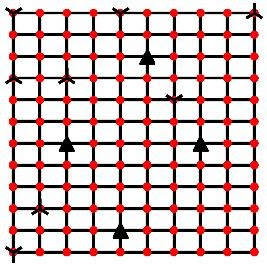
\includegraphics[width = 1\textwidth]{Figures/10x12simple_plane.jpg}
    \caption{Plane rectangular lattice}
    \label{fig:plane_rectangular}
\end{minipage}
\hspace{5mm}
\begin{minipage}{0.3\textwidth}
    \centering
    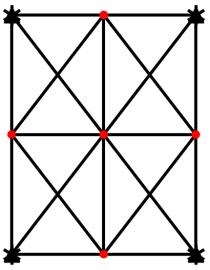
\includegraphics[width = 1\textwidth]{Figures/3x3braced_plane.jpg}
    \caption{Plane rectangular lattice with both bracing}
    \label{fig:Plane_rect_with_bracing1}
\end{minipage}
\hspace{5mm}
\begin{minipage}{0.3\textwidth}
    \centering
    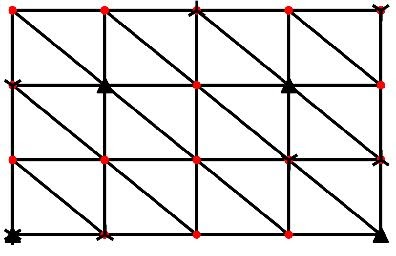
\includegraphics[width = 1\textwidth]{Figures/5x4_braced_plane.jpg}
    \caption{Plane rectangular lattice with one bracing}
    \label{fig:Plane_rect_with_bracing2}
\end{minipage}
\end{figure}

\begin{figure}[!htbp]
\begin{minipage}{0.3\textwidth}
    \centering
    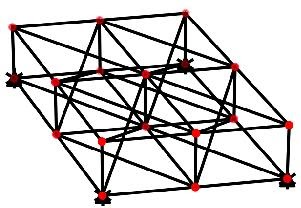
\includegraphics[width = 1\textwidth]{Figures/3x3reduced_bracings3d.jpg}
    \caption{3D rectangular lattice with few braces}
    \label{fig:3D_rect1}
\end{minipage}
\hspace{5mm}
\begin{minipage}{0.3\textwidth}
    \centering
    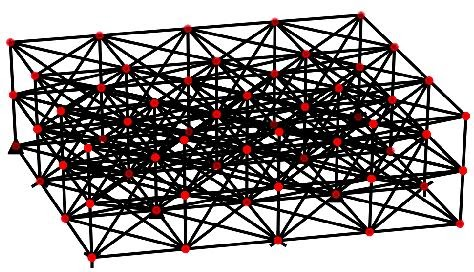
\includegraphics[width = 1\textwidth]{Figures/5x43d3layer.jpg}
    \caption{3D rectangular 3-layer lattice with braces}
    \label{fig:3d_rect2}
\end{minipage}
\hspace{5mm}
\begin{minipage}{0.3\textwidth}
    \centering
    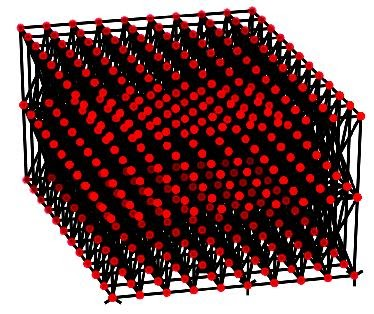
\includegraphics[width = 1\textwidth]{Figures/10x12braced3d3layer.jpg}
    \caption{3D rectangualar 3-layer lattice with all possible braces}
    \label{fig:3d_rect3}
\end{minipage}
\end{figure}

\section{Model Details}
The model works on energy minimization principles and can simulate all kind of strain fields and loading. The model uses L-BFGS-B optimization algorithm from scipy.optimize toolbox of Python. Broyden–Fletcher–Goldfarb–Shanno (BFGS) algorithm is an iterative method for solving unconstrained nonlinear optimization problems. L-BFGS-B is Limited memory-BFGS algorithm extended to handle simple box constraints (support conditions in our case). All the models and results presented in this study are for simple supported on all edges of plate condition. 

Design variables are the coordinates of the nodes stacked together. These variable determine the length of the springs in any given state which in turn determines the energy of the system.

Energy of the system is defined as:
\begin{equation}
    E = \sum_{i = 1}^{N}\frac{1}{2}k_i (l_i - l_{0i})^2 - \boldsymbol{f.\Delta r}
\end{equation}
where:\\
\\
    $E$: Total energy of the system\\
    $N$: total number of springs\\
    $K_i$: Stiffness of the $i^{th}$ spring\\
    $l_i$: current length of $i^{th}$ spring\\
    $l_{0i}$: Natural length of $i^{th}$ spring\\
    $\boldsymbol{f}$: Load vector\\
    $\Delta r$: Displacement vector\\
    
The optimization program also uses the derivatives, which are given as:
\begin{equation}
    \frac{\partial E}{\partial x_i} = \sum_{j \in T_i} k_j(x_j - x_{0j})(1 - \frac{l_{0j}}{\sqrt{(x_j - x_{0j})^2 + (y_j - y_{0j})^2 + (z_j - z_{0j})^2}}) - f_{x_i}
\end{equation}
\begin{equation}
    \frac{\partial E}{\partial y_i} = \sum_{j \in T_i} k_j(y_j - y_{0j})(1 - \frac{l_{0j}}{\sqrt{(x_j - x_{0j})^2 + (y_j - y_{0j})^2 + (z_j - z_{0j})^2}}) - f_{y_i}
\end{equation}
\begin{equation}
    \frac{\partial E}{\partial z_i} = \sum_{j \in T_i} k_j(z_j - z_{0j})(1 - \frac{l_{0j}}{\sqrt{(x_j - x_{0j})^2 + (y_j - y_{0j})^2 + (z_j - z_{0j})^2}}) - f_{z_i}
\end{equation}

where\\
$T_i$: set of all springs connected to node $i$\\
$f_{x_i}$, $f_{y_i}$, and $f_{z_i}$: force at node $i$ in $X-$, $Y-$, and $Z-$ directions respectively

\section{Theory}
The models are validated for point load at centre using Classical Plate Theory (CPT), also known as Kirchhoff-Love theory and First-order Shear deformation Theory (FSDT), also known as Mindlin–Reissner plate theory. A point load applied at the centre of the plate is used for the calibration and validation. More details about the models are in their respective sections.\cite{reddy2006theory}\cite{timoshenko1959theory}

\subsection{Classical Plate Theory}
According to classical plate theory, displacement field is based on the following assumptions, called Kirchhoff hypothesis:
\begin{enumerate}
    \item Straight line perpendicular to the mid-surface (i.e., transverse normals) before deformation remain straight after deformation.
    \item The transverse normals do not experience elongation (i.e., they are in inextensible).
    \item The transverse normals rotate such that they remain perpendicular to middle surface after deformation.
\end{enumerate}

Following these assumptions, the strains are found to be as given in eq~\ref{eq:CPT_strain1} - eq~\ref{eq:CPT_strains_last}.

\begin{equation}
    \epsilon_{xx} = \frac{\partial u_0}{\partial x} + \frac{1}{2}(\frac{\partial w_0}{\partial x})^2 - z\frac{\partial^2 w_0}{\partial x^2}
    \label{eq:CPT_strain1}
\end{equation}
\begin{equation}
    \epsilon_{yy} = \frac{\partial v_0}{\partial y} + \frac{1}{2}(\frac{\partial w_0}{\partial y})^2 - z\frac{\partial^2 w_0}{\partial y^2}
\end{equation}
\begin{equation}
    \epsilon_{zz} = \frac{1}{2}(\frac{\partial u_0}{\partial y} + \frac{\partial v_0}{\partial x} + \frac{\partial w_0}{\partial x}\frac{\partial w_0}{\partial y} - 2z\frac{\partial^2 w_0}{\partial x\partial y})
\end{equation}
\begin{equation}
    \epsilon_{xz} = \epsilon_{yz} = \epsilon_{zz} = 0
    \label{eq:CPT_strains_last}
\end{equation}

Using the principle of virtual displacement and strains defined above, the governing equation for CPT is obtained as eq~\ref{eq:gov_eqn} for a homogenous isotropic plate.

\begin{equation}
    \label{eq:gov_eqn}
    D\nabla^2\nabla^2 w_0 + kw_0 = q - \frac{1}{ 1 - \nu}\nabla^2 M_T
\end{equation}
where\\
\begin{equation}
    D = \frac{Eh^3}{12(1 - \nu^2)}
    \label{eq:D}
\end{equation}

using Navier's solution for a point load of magnitude $Q_0$ applied at the centre of a square plate simply supported on all four edges of dimension $a$, the analytical equation obtained for transverse displacement at centre using first ten element of the series is:
\begin{equation}
    w_0(x_c, y_c) = 0.0116\frac{Q_0a^2}{D}
    \label{eq:w_CPT}
\end{equation}

Eq~\ref{eq:w_CPT} will be used to calibrate and validate the model as shown later.

\subsection{First-order Shear Deformation Theory}
The first-order shear deformation theory is arrived at by relaxing the third assumption of the Kirchhoff-Love plate theory, which states that transverse normal remain perpendicular to middle surface after deformation, by allowing for an arbitrary constant rotation of transverse normals. The assumption that transverse normals remain straight after deformation holds for first order theory by can be dismissed by using higher order theories.

using the modified assumptions, the strains are as following:

\begin{equation}
    \epsilon_{xx} = \frac{\partial u_0}{\partial x} + \frac{1}{2}(\frac{\partial w_0}{\partial x})^2 + z\frac{\partial\phi_x}{\partial x}
    \label{eq:FSDT_strain1}
\end{equation}
\begin{equation}
    \epsilon_{yy} = \frac{\partial v_0}{\partial y} + \frac{1}{2}(\frac{\partial w_0}{\partial y})^2 + z\frac{\partial\phi_y}{\partial y}
\end{equation}
\begin{equation}
    \epsilon_{zz} = 0
    \label{eq:strain_z_FSDT}
\end{equation}
\begin{equation}
    \gamma_{xy} = (\frac{\partial u_0}{\partial y} + \frac{\partial v_0}{\partial x} + \frac{\partial w_0}{\partial x}\frac{\partial w_0}{\partial y}) - z(\frac{\partial\phi_x}{\partial y} + \frac{\partial\phi_y}{\partial x})
\end{equation}
\begin{equation}
    \gamma_{xz} = \frac{\partial w_0}{\partial x} + \phi_x
\end{equation}
\begin{equation}
    \gamma_{yz} = \frac{\partial w_0}{\partial y} + \phi_y
    \label{eq:FSDT_last}
\end{equation}

Using the strains from eq~\ref{eq:FSDT_strain1} - eq~\ref{eq:FSDT_last}, for small deflection and rotation, we get governing equation for bending as,

\begin{equation}
    K_sGh(\Delta^2w_0 + \frac{\partial\phi_x}{\partial x} + \frac{\partial\phi_y}{\partial y}) + q(x, y) = 0
    \label{eq:gov_eq_FSDT1}
\end{equation}
\begin{equation}
    D(\frac{\partial^2\phi_x}{\partial x^2} + \nu\frac{\partial^2\phi_y}{\partial x\partial y}) + \frac{D(1 - \nu)}{2}(\frac{\partial^2\phi_x}{\partial y^2} + \frac{\partial^2\phi_y}{\partial x\partial y}) - K_sGh(\frac{\partial w_0}{\partial x} + \phi_x) = 0
\end{equation}
\begin{equation}
    \frac{Gh^3}{12}(\frac{\partial^2\phi_x}{\partial x\partial y} + \frac{\partial^2\phi_y}{\partial x^2}) + D(\nu\frac{\partial^2\phi_x}{\partial x\partial y} + \frac{\partial^2\phi_y}{\partial y^2}) - K_sGh(\frac{\partial w_0}{\partial y} + \phi_y) = 0
    \label{eq:gov_eq_FSDT3}
\end{equation}

The solution to the eq~\ref{eq:gov_eq_FSDT1} - eq~\ref{eq:gov_eq_FSDT3} is obtained for the case of point load applied at the centre is obtained using Navier Solution. 

\section{Models and Results}
To validate the Python program and models developed, deflections resulting from a point load applied at the centre are checked with respect to analytical solutions available from theories described above. Following the comparison, possible reason for deviations, limitations and advantages are discussed.

The study is carried out with three kinds of model. Further, each model has three variant with varying number number of nodes and springs. Two types of studies are carried out for each variant, namely Constant Stiffness studies in which springs have constant stiffness irrespective of its length, and Constant Axial rigidity studies in which $EA$ is held constant for springs and their stiffness$(= EA/l)$ is inversely proportional to their lengths. Also to ensure that $\epsilon_{zz}$ is zero or at least close to zero (eq~\ref{eq:strain_z_FSDT} and eq~\ref{eq:CPT_strains_last}) the vertical spring are provided with stiffness orders of magnitude higher than in plane spring stiffness. Details of each of them can be found in their respective sections.

\subsection{Model 1}
The model 1 is composed of of a 3-layer simple cubic lattice type model. Dimension of the plate is 1~m x 1~m x 0.02~m. Stiffness of the springs in model are calibrated for displacement at centre for a 2 kN point load applied at centre with displacements at centre of an equivalent plate with $E = 2$ GPa and $\nu = 0.25$).

\subsubsection{Model 1 - Type A}
These models are type 1 model with 4 x 4 x 2 structure of cuboids of dimension 0.25~m x 0.25~m x 0.01~m stacked together as shown in the fig~\ref{fig:M1_a_XY} - fig~\ref{fig:M1_a_3D}.

\begin{figure}[!htbp]
\begin{minipage}{0.3\textwidth}
    \centering
    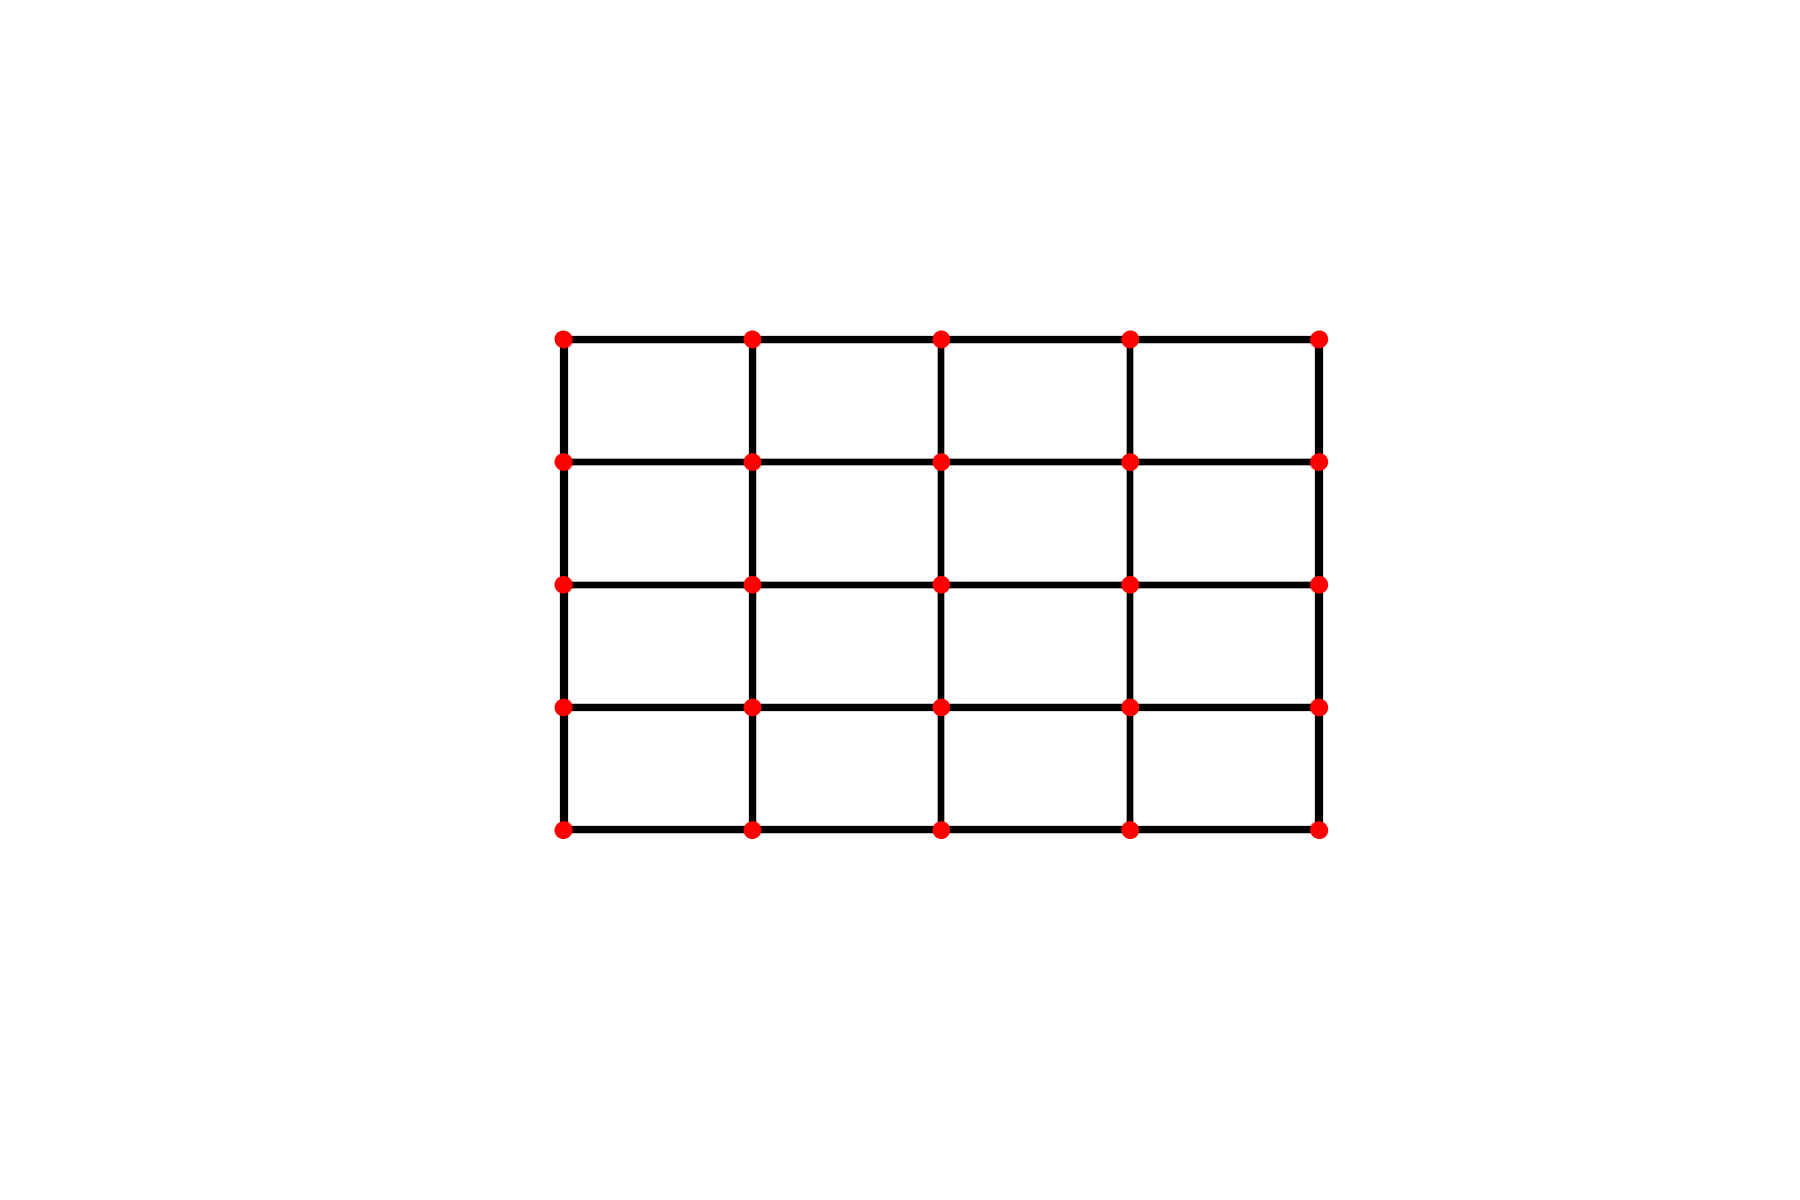
\includegraphics[width = 1\textwidth]{Figures/M1_type_a_XY.png}
    \caption{Model 1 - Type A - XY Projection}
    \label{fig:M1_a_XY}
\end{minipage}
\hspace{5mm}
\begin{minipage}{0.3\textwidth}
    \centering
    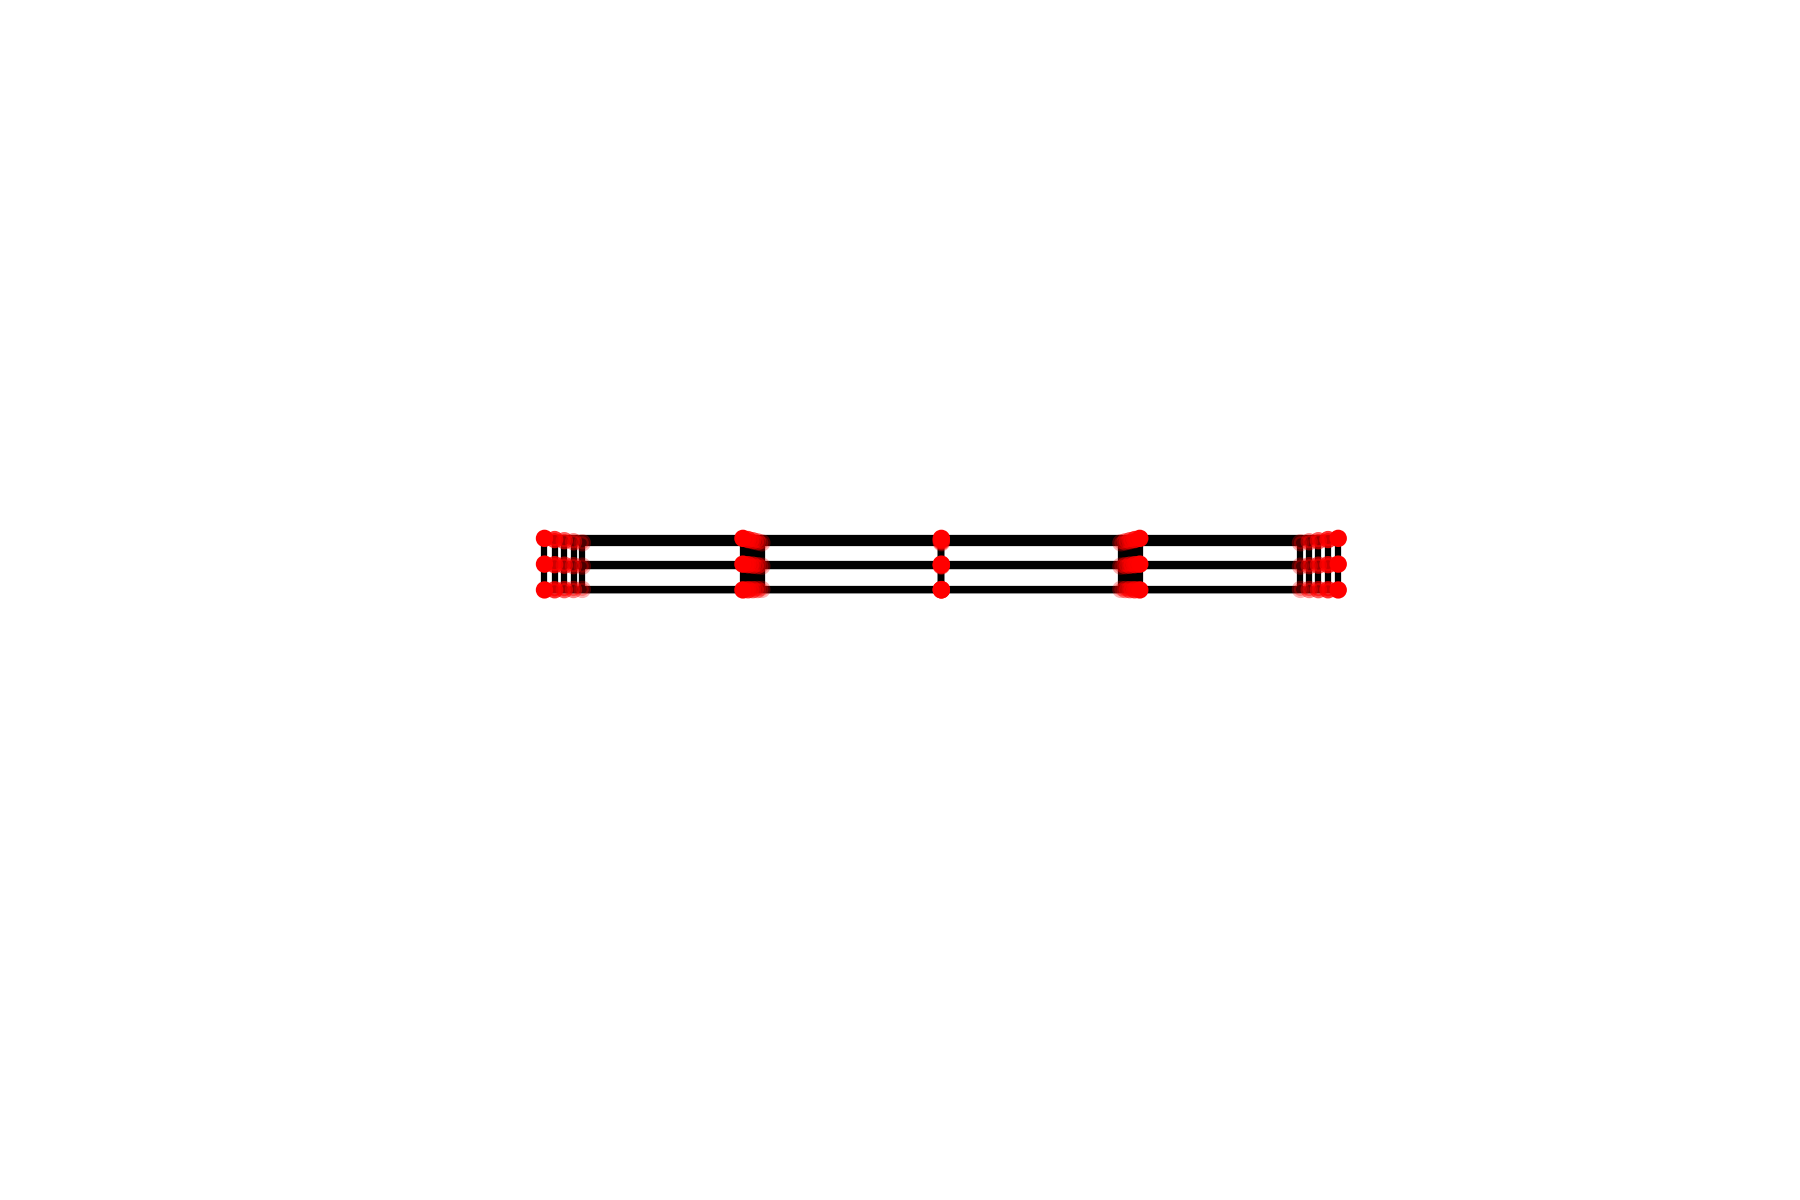
\includegraphics[width = 1\textwidth]{Figures/M1_type_a_YZ.png}
    \caption{Model 1 - Type A - YZ Projection}
    \label{fig:M1_a_YZ}
\end{minipage}
\hspace{5mm}
\begin{minipage}{0.3\textwidth}
    \centering
    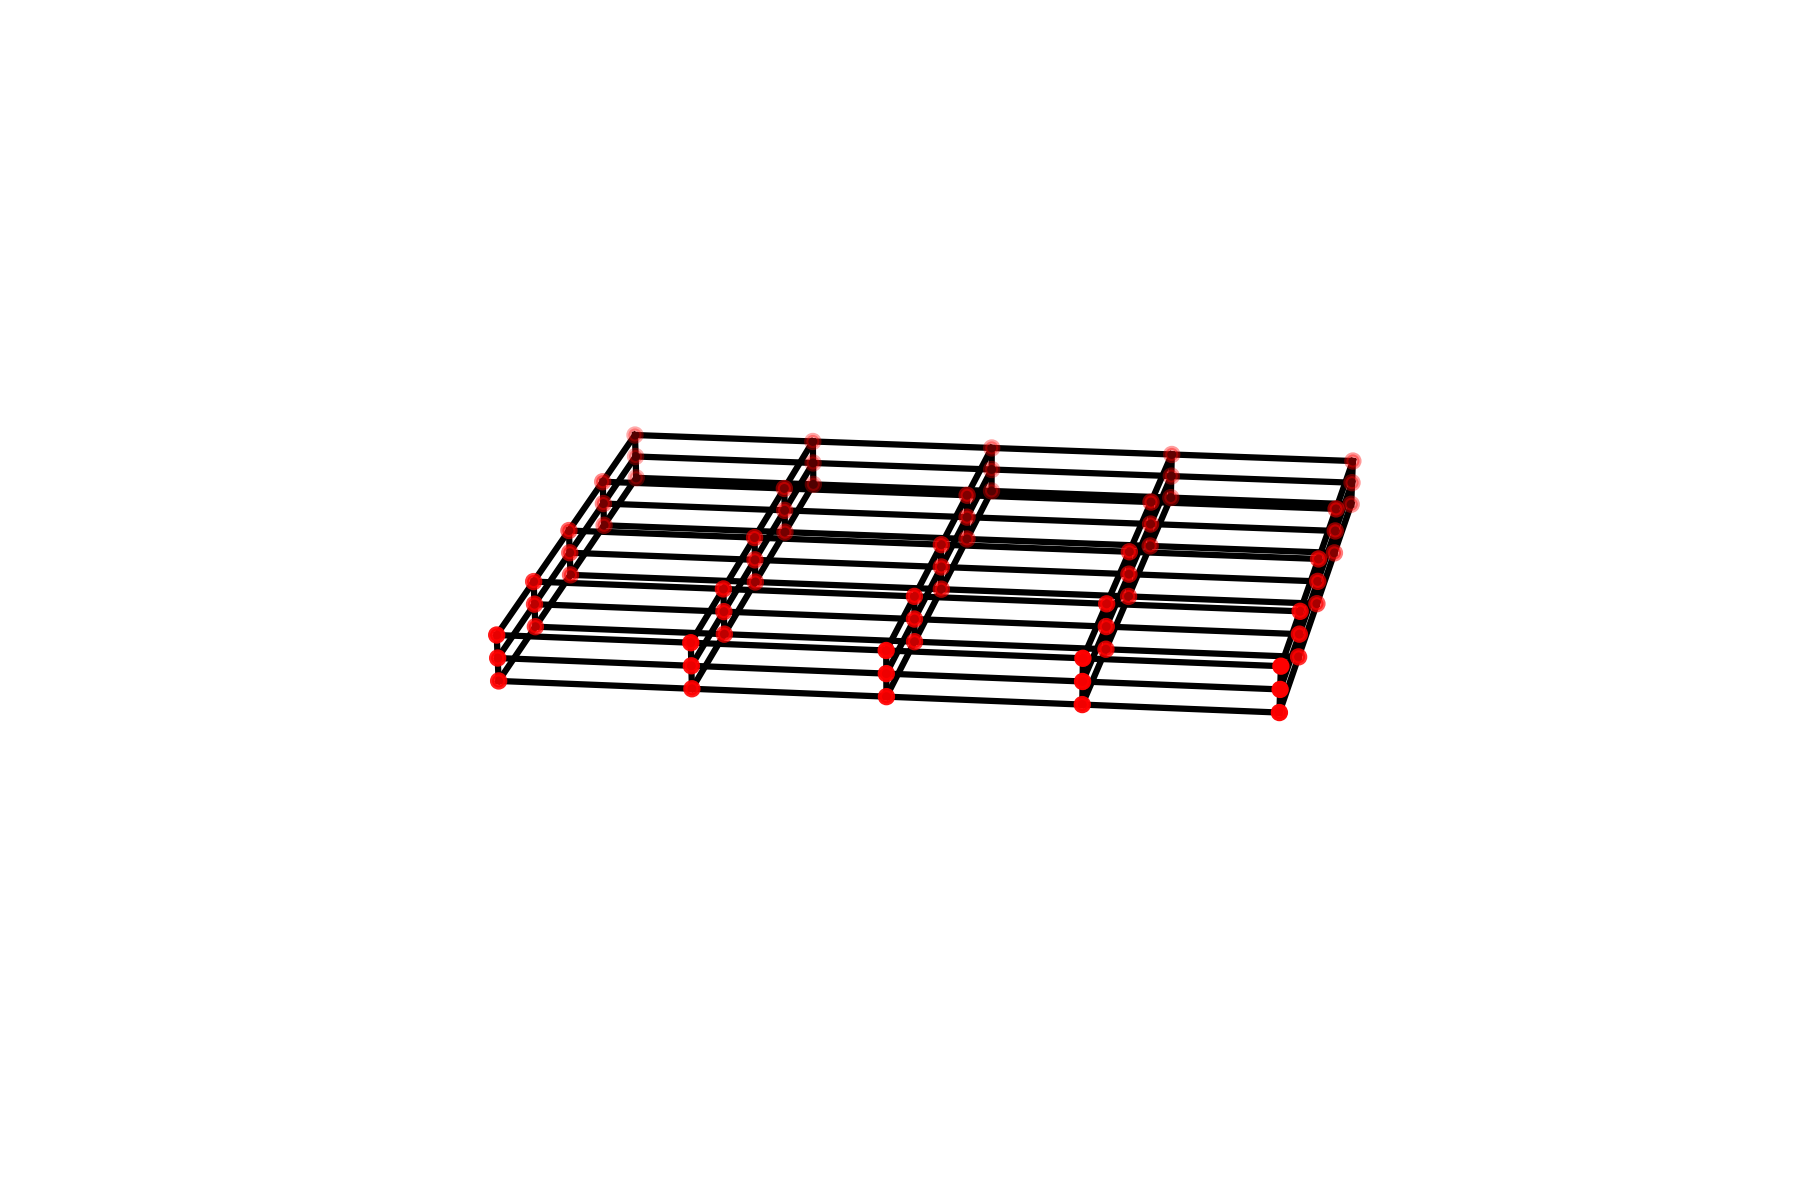
\includegraphics[width = 1\textwidth]{Figures/M1_type_a_3D.png}
    \caption{Model 1 - Type A - 3D View}
    \label{fig:M1_a_3D}
\end{minipage}
\end{figure}

The plots for vertical deflections at centre with respect to point load applied at the centre for Constant Stiffness and Constant Axial rigidity are shown in the fig~\ref{fig:M1_a_plt}.

\begin{figure}[!htbp]
    \centering
    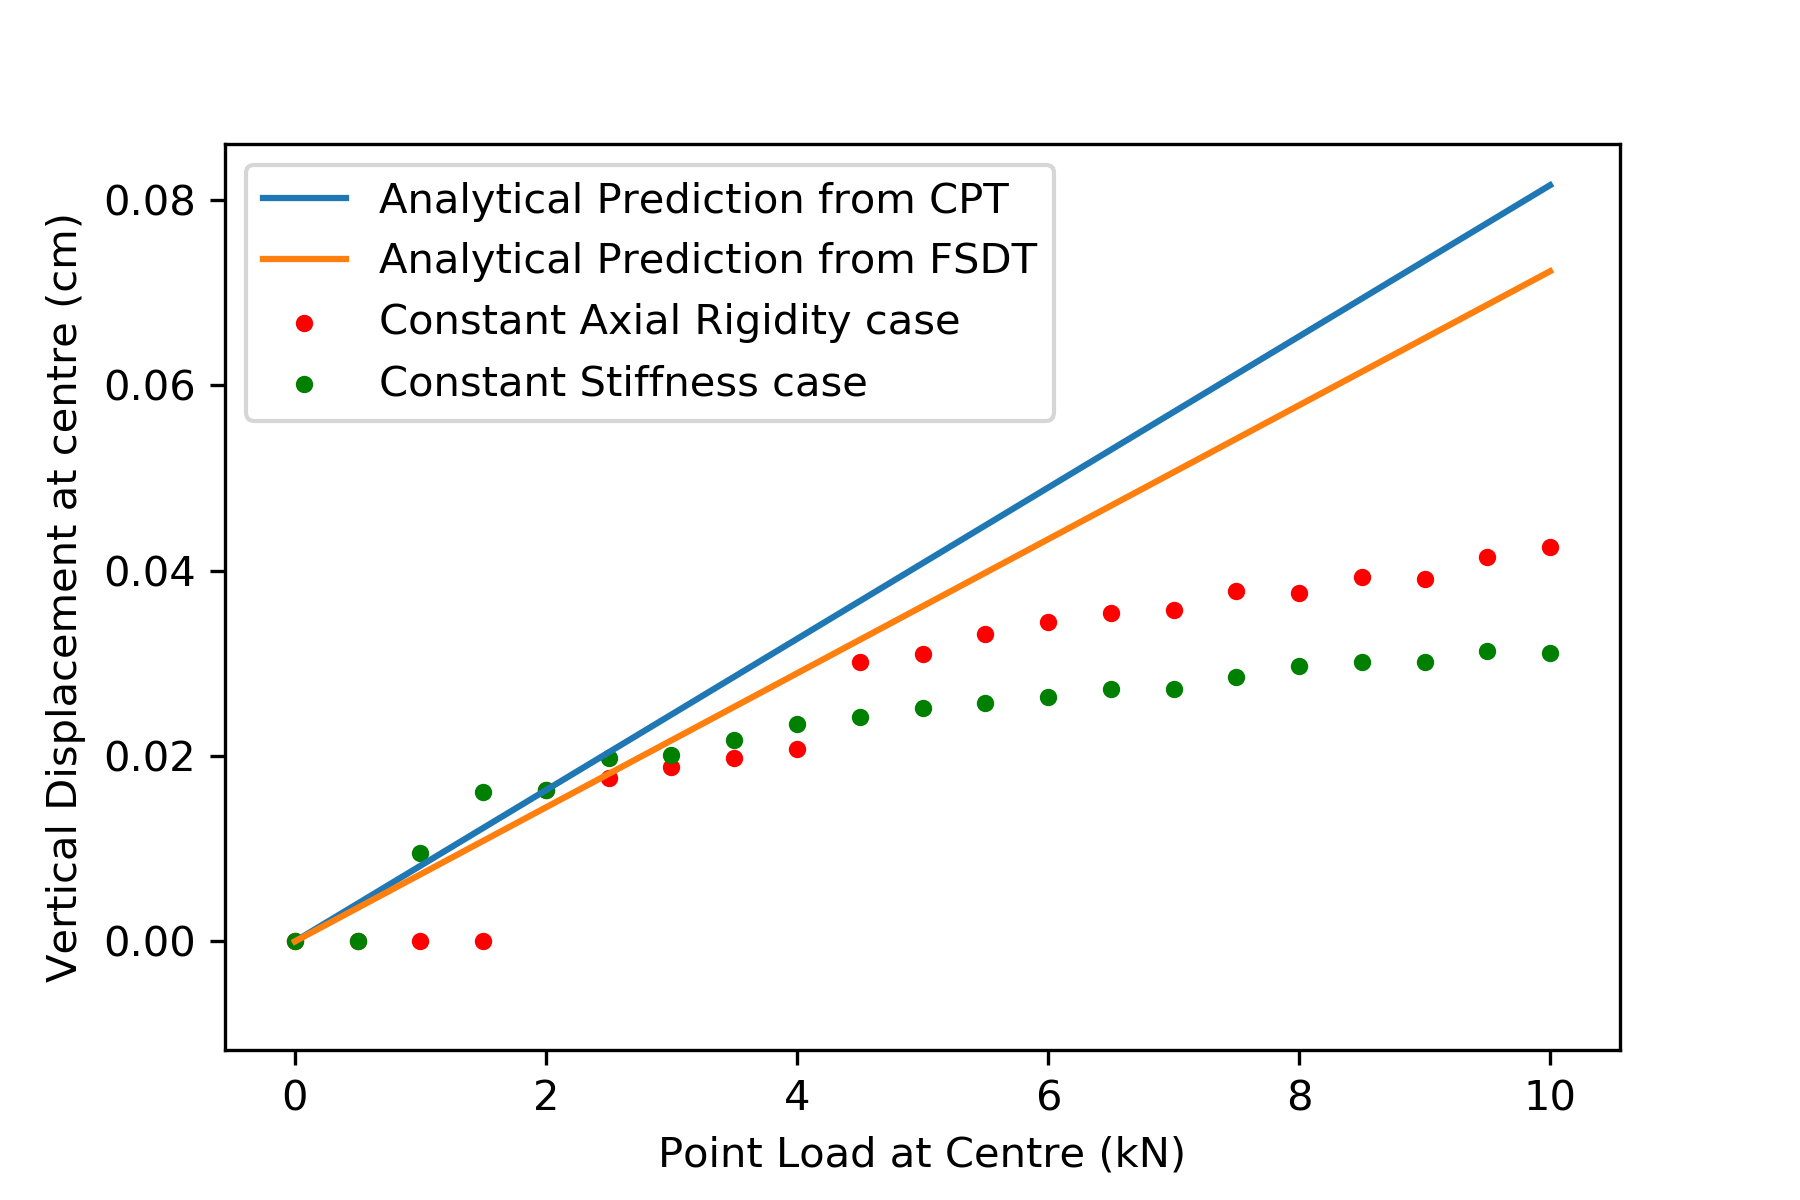
\includegraphics[width = 0.9\textwidth]{Figures/M1_a_plt.png}
    \caption{Model 1 - Type A - vertical Displacement with respect to Point Load at centre}
    \label{fig:M1_a_plt}
\end{figure}

\begin{figure}[!htbp]
    \centering
    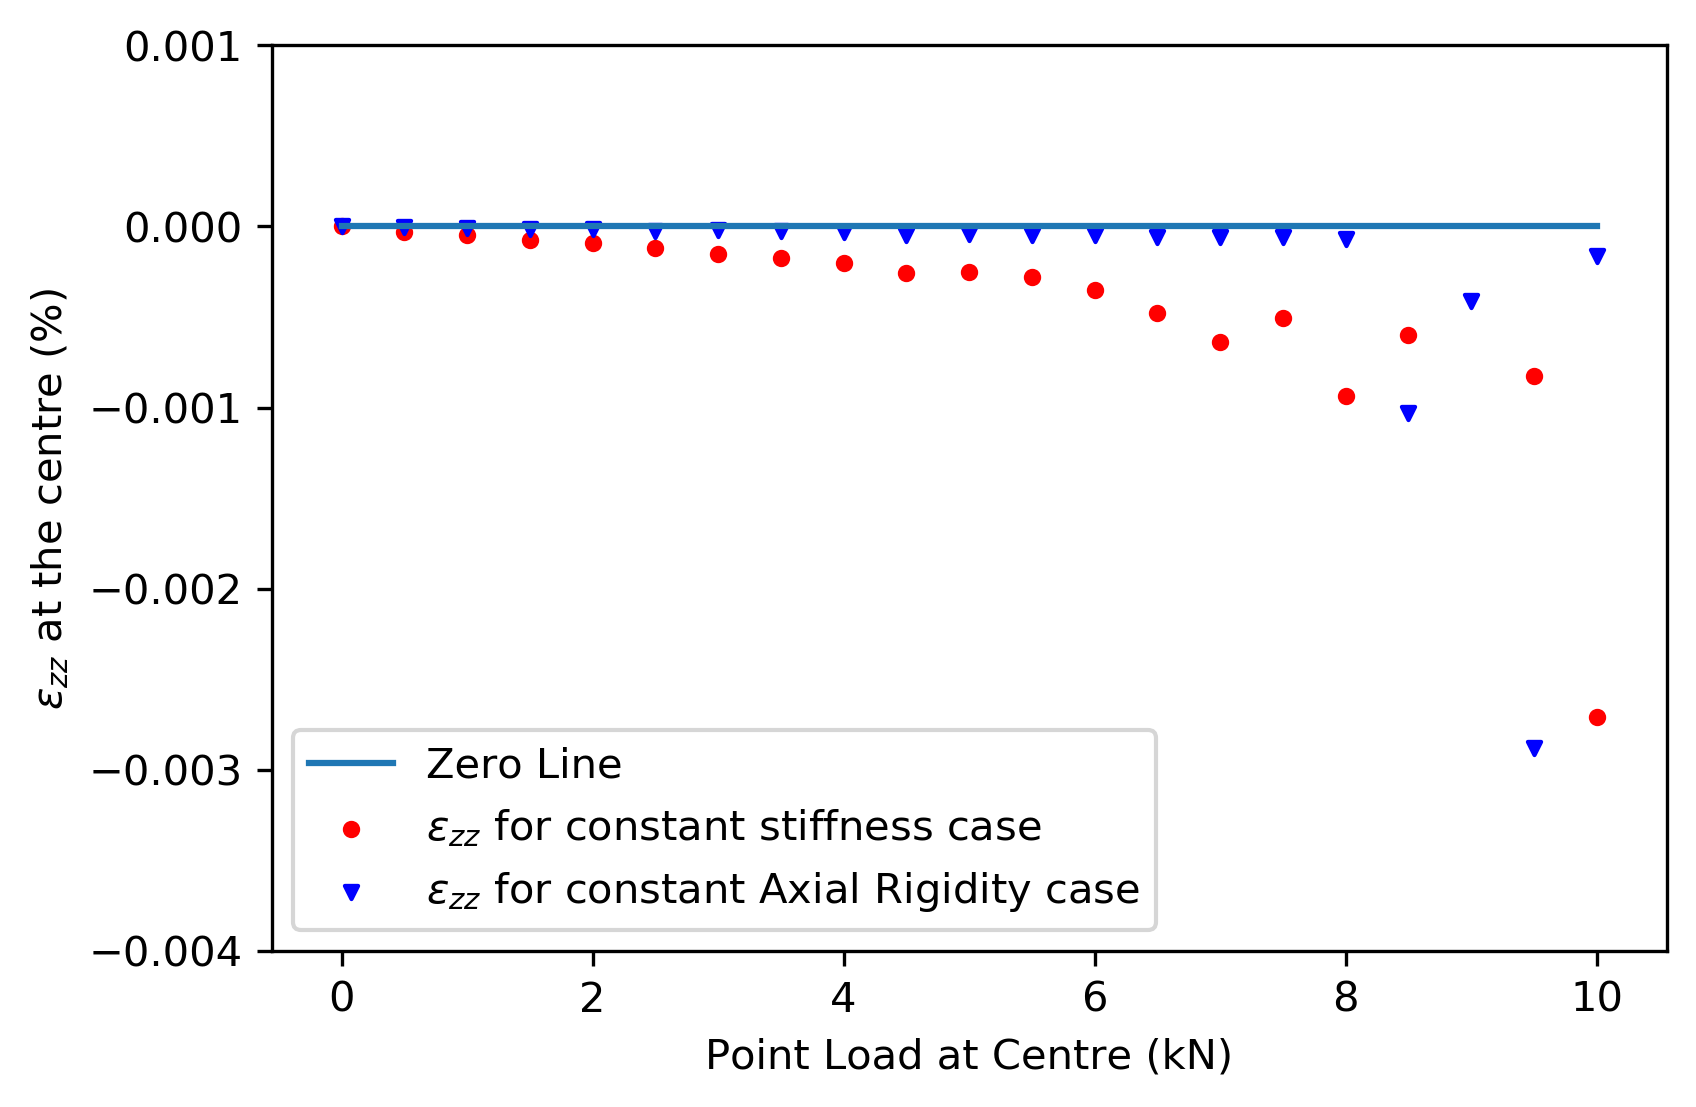
\includegraphics[width = 0.9\textwidth]{Figures/M1_a_strain.png}
    \caption{Model 1 - Type A - $\epsilon_{zz}$ with respect to Point Load at centre}
    \label{fig:M1_a_strain_plt}
\end{figure}

As it can be seen from the fig~\ref{fig:M1_a_plt}, there are significant deviations from the analytical results. The zero initial values corresponding to lower load are due to numerical difficulties in which the values in the associated matrices differ by order of magnitude and as a result are ill conditioned. This results in almost singular matrices which lead to zero displacements even when the load is applied. Also, the model underestimates the displacements at larger force magnitudes, and the predictions lie closer to the analytical solution obtained by First-order Shear Deformation Theory (FSDT) than Classical Plate Theory (CPT). This behavior can be attributed to the deviation of $\epsilon_{zz}$ from zero values (eq~\ref{eq:CPT_strains_last} and eq~\ref{eq:strain_z_FSDT} as shown in fig~\ref{fig:M1_a_strain_plt}, and non linear behavior (reaction response) of horizontal spring system as they undergo displacements in vertical direction.
%see if this can be included in appendix

\begin{figure}[!htbp]
    \centering
    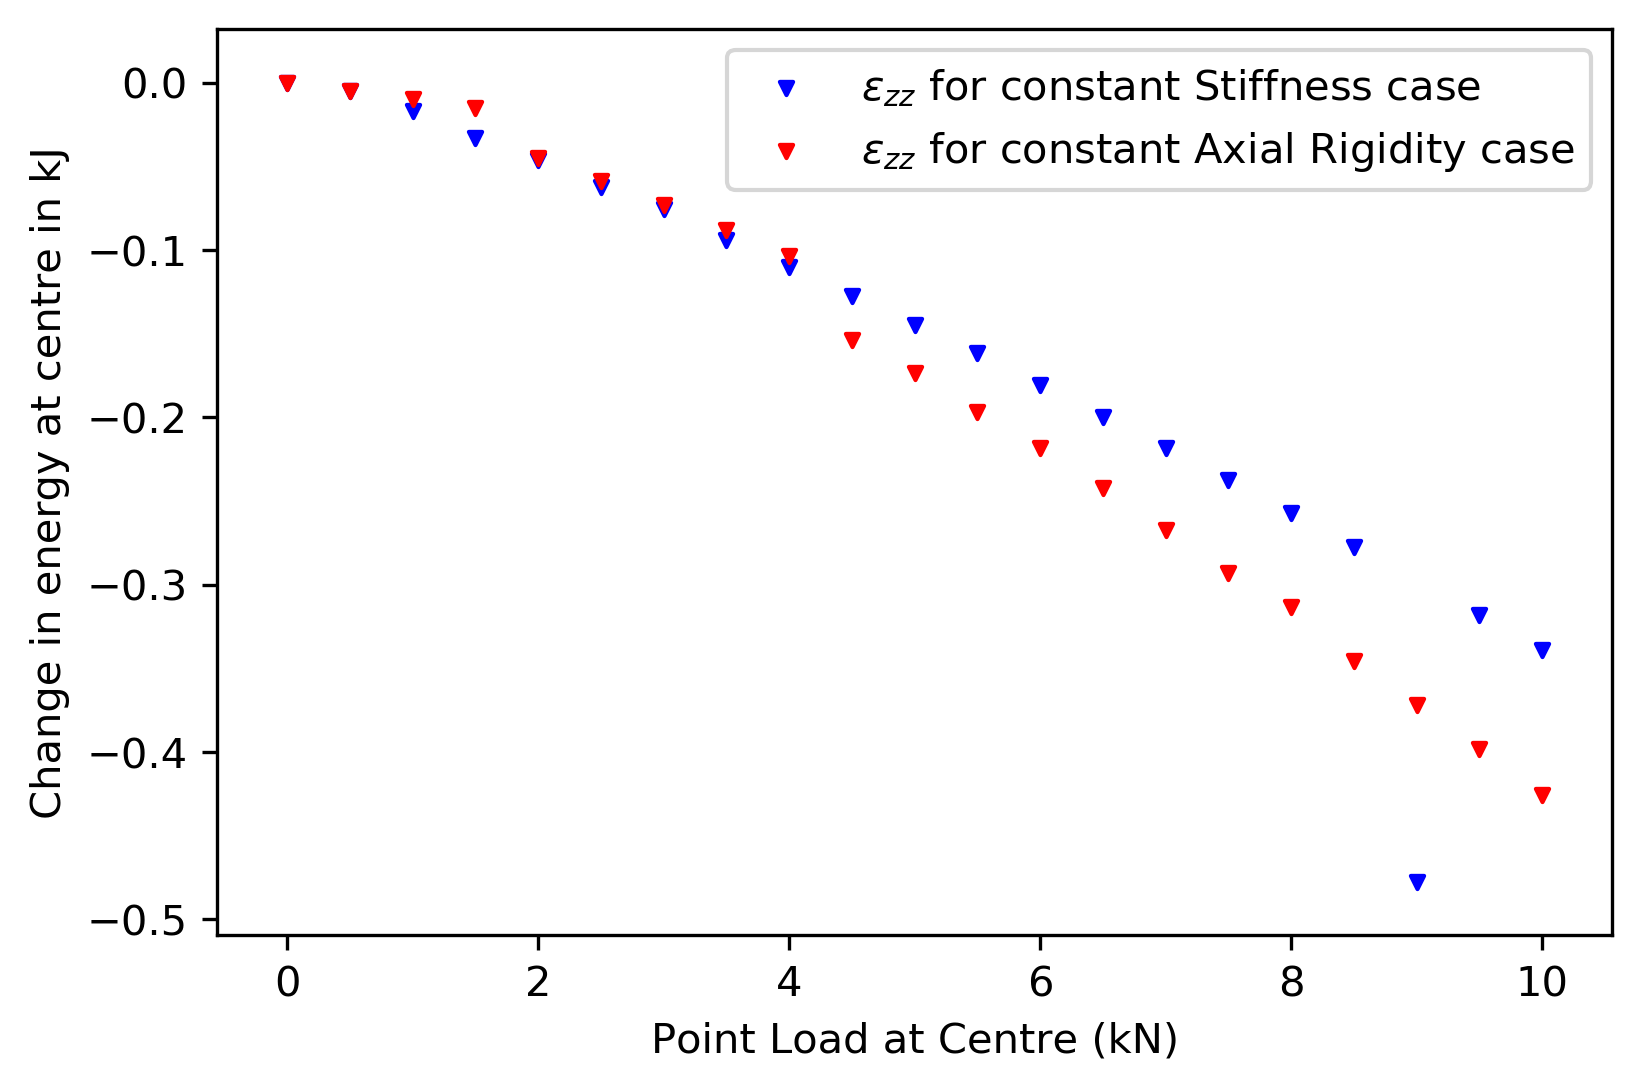
\includegraphics[width = 0.9\textwidth]{Figures/M1_a_energy.png}
    \caption{Model 1 - Type A - Change in Energy with respect to Point Load at centre}
    \label{fig:M1_a_energy}
\end{figure}

In fig~\ref{fig:M1_a_energy}, energies in the undeformed states for all forces are zero.

\subsubsection{Model 1 - Type B}
Model 1 - Type B is 10 x 10 x 2 structure of Model 1 cuboids of dimensions 0.1~m x 0.1~m x 0.01~m. The model is shown in fig~\ref{fig:M1_b_XY} - fig~\ref{fig:M1_b_3D}

\begin{figure}[!htbp]
\begin{minipage}{0.3\textwidth}
    \centering
    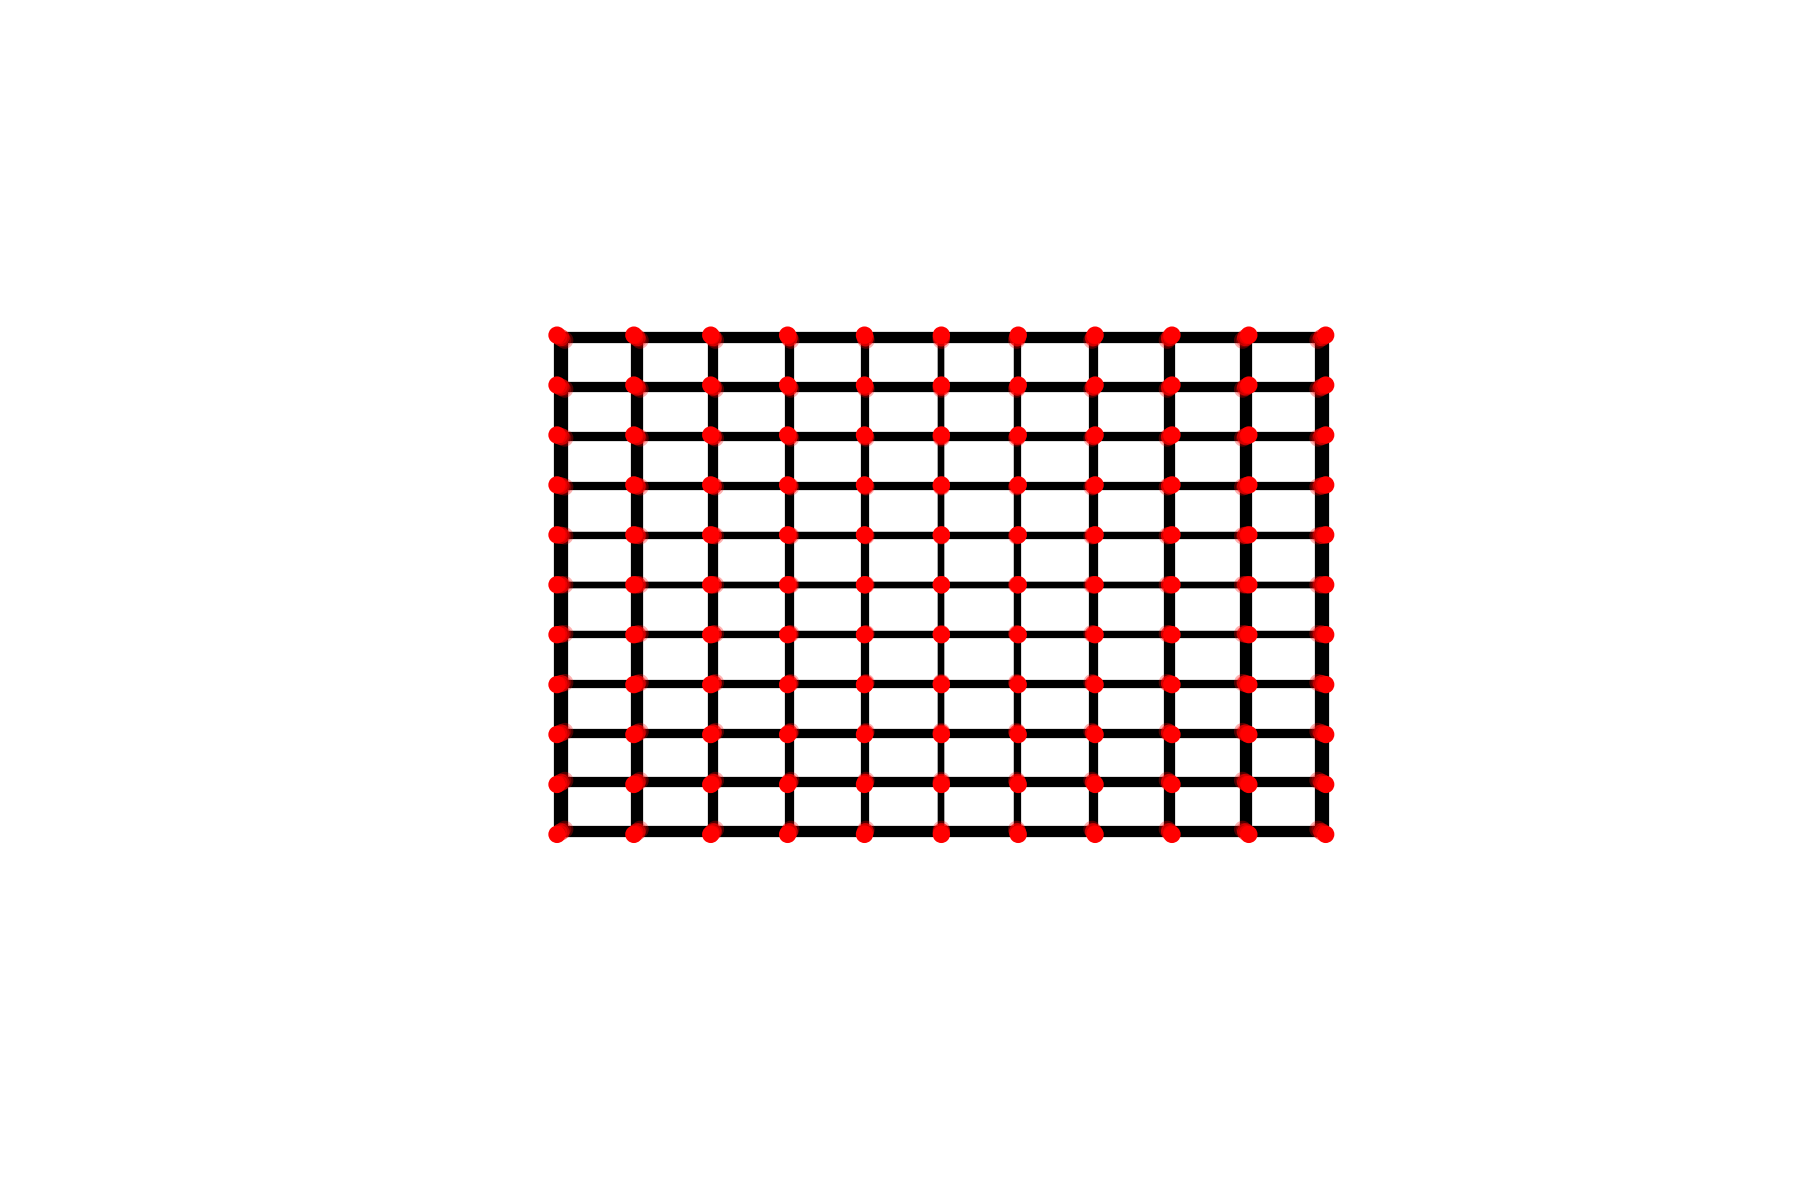
\includegraphics[width = 1\textwidth]{Figures/M1_b_XY.png}
    \caption{Model 1 - Type B - XY Projection}
    \label{fig:M1_b_XY}
\end{minipage}
\hspace{5mm}
\begin{minipage}{0.3\textwidth}
    \centering
    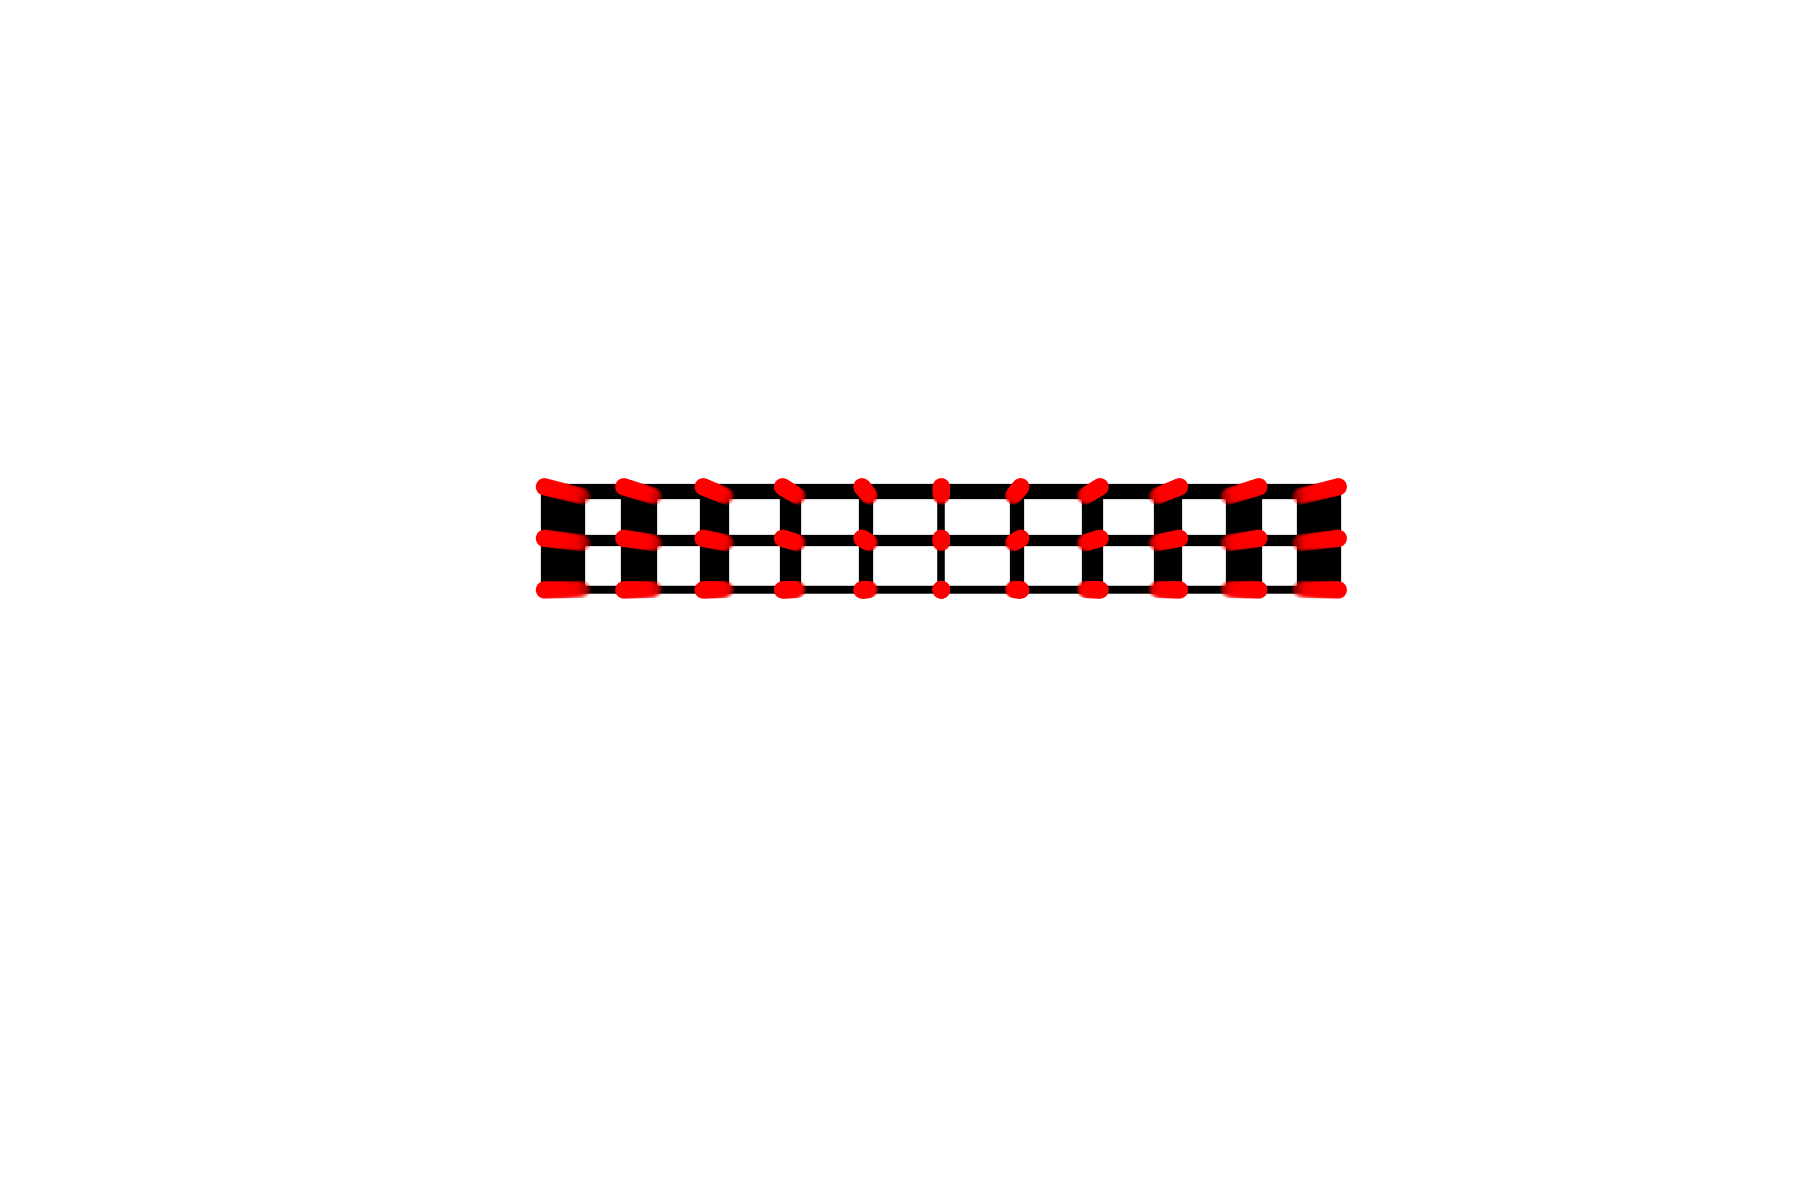
\includegraphics[width = 1\textwidth]{Figures/M1_b_YZ.png}
    \caption{Model 1 - Type B - YZ Projection}
    \label{fig:M1_b_YZ}
\end{minipage}
\hspace{5mm}
\begin{minipage}{0.3\textwidth}
    \centering
    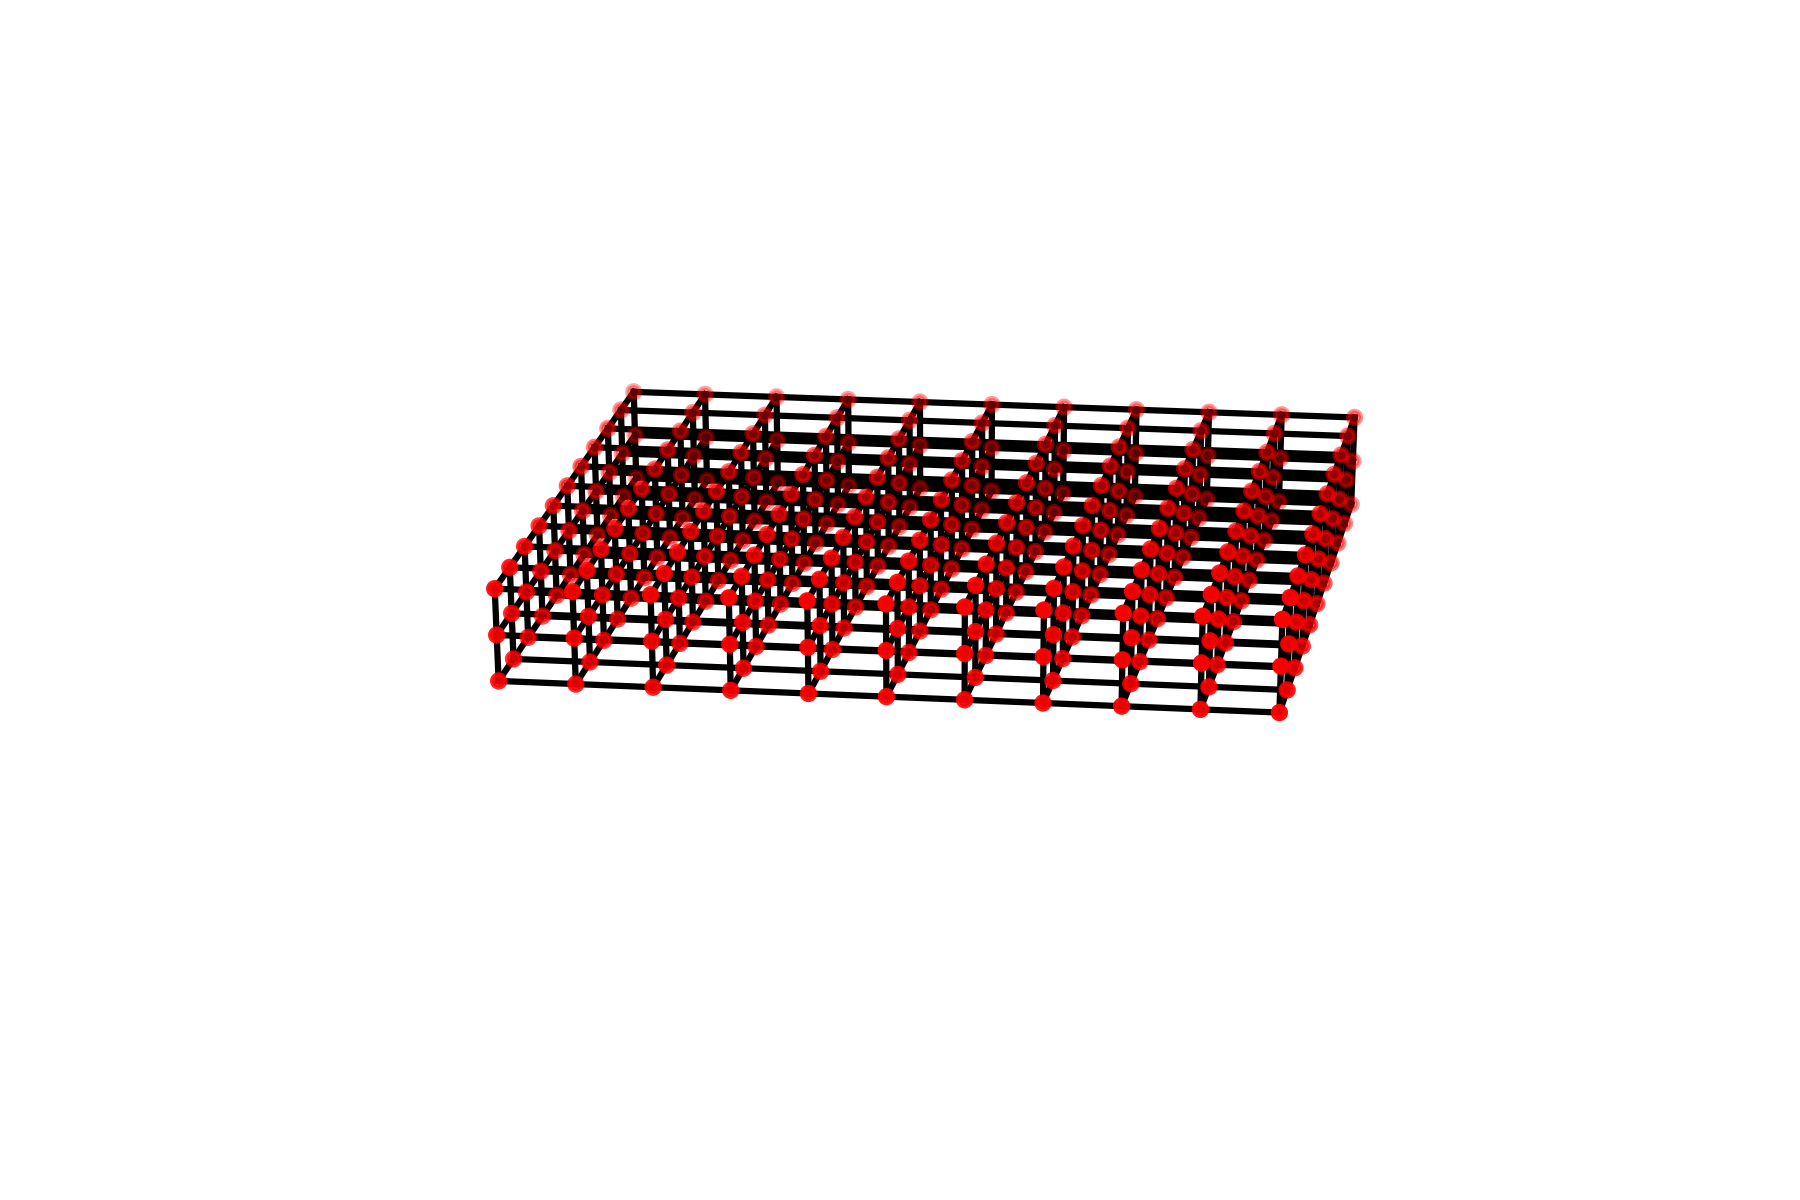
\includegraphics[width = 1\textwidth]{Figures/M1_b_3D.png}
    \caption{Model 1 - Type B - 3D View}
    \label{fig:M1_b_3D}
\end{minipage}
\end{figure}

The plots corresponding to Model 1 - Type B are shown in fig~\ref{fig:M1_b_plt} - fig~\ref{fig:M1_b_energy}.

\begin{figure}[!htbp]
    \centering
    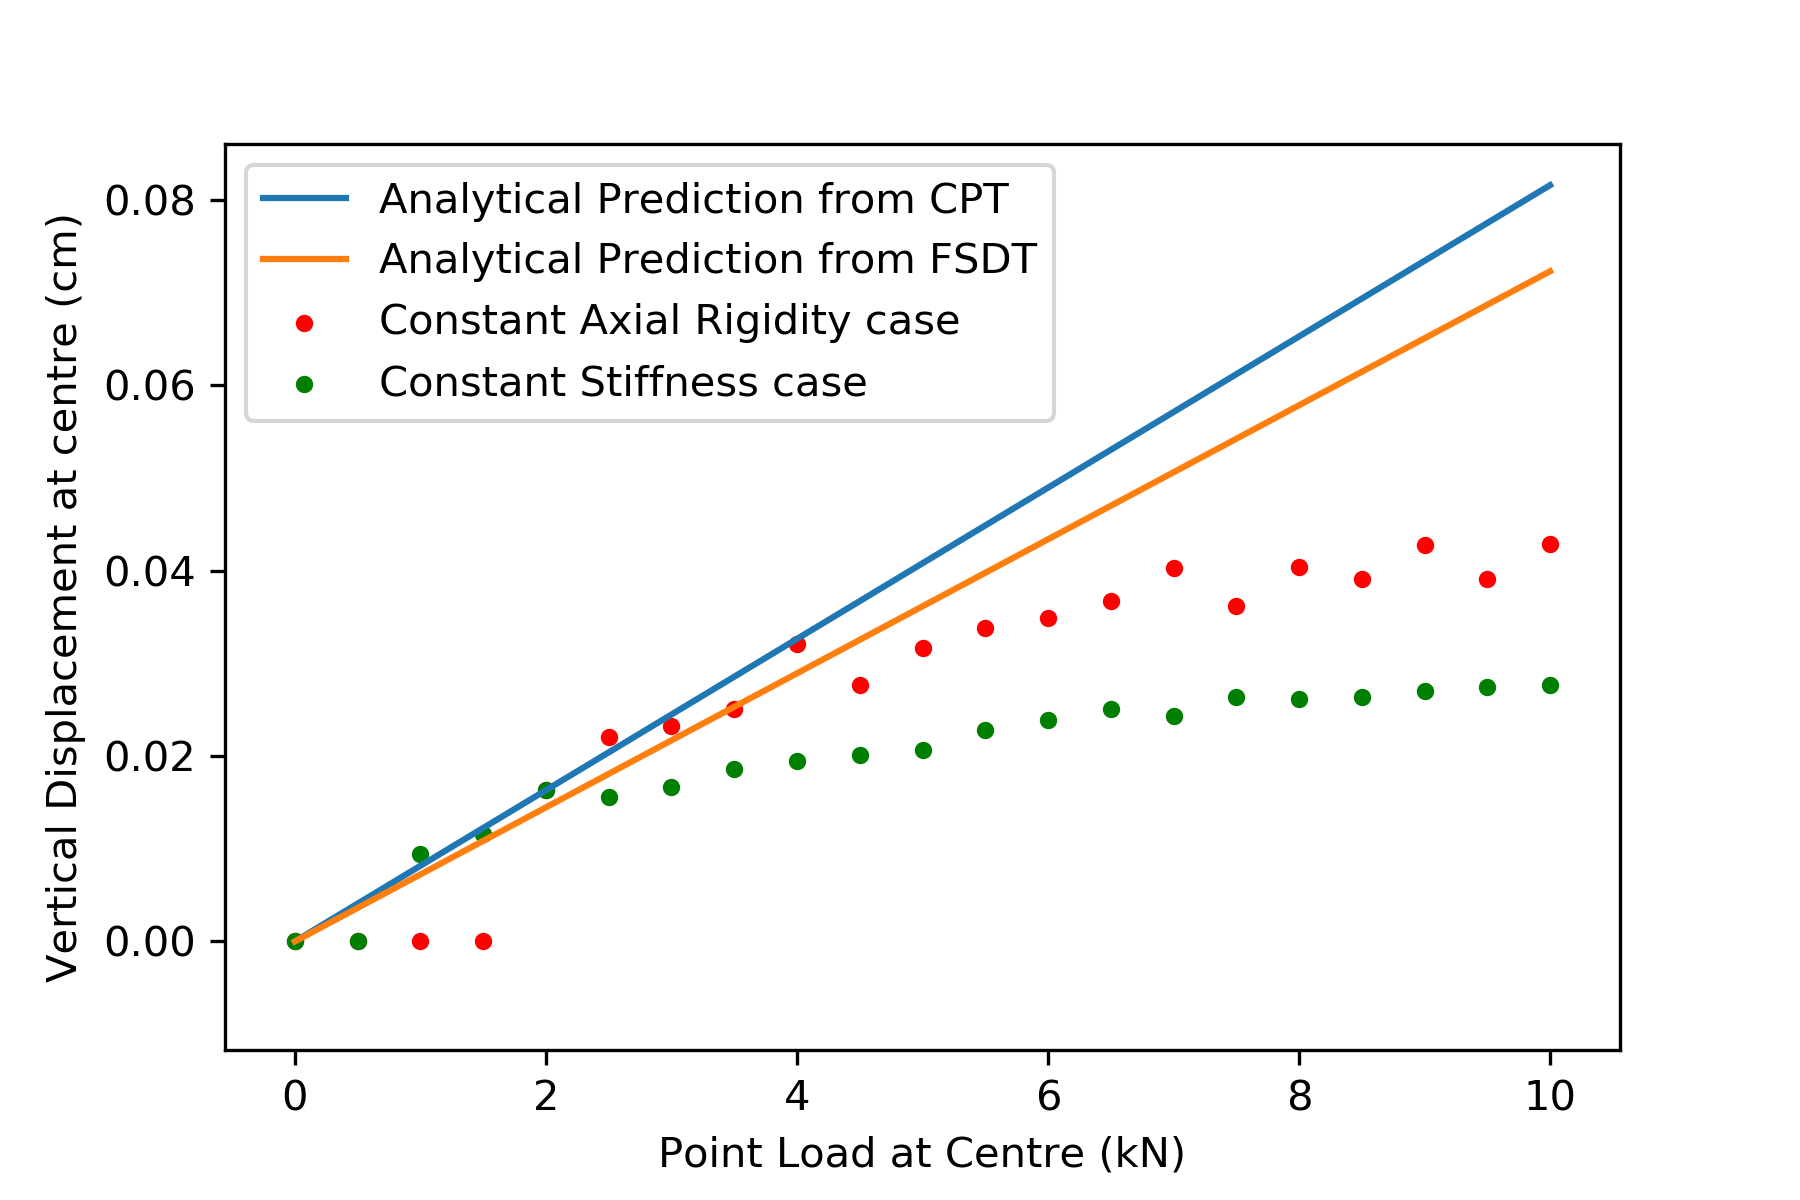
\includegraphics[width = 0.8\textwidth]{Figures/M1_b_plt.png}
    \caption{Model 1 - Type B - vertical Displacement with respect to Point Load at centre}
    \label{fig:M1_b_plt}
\end{figure}

\begin{figure}[!htbp]
    \centering
    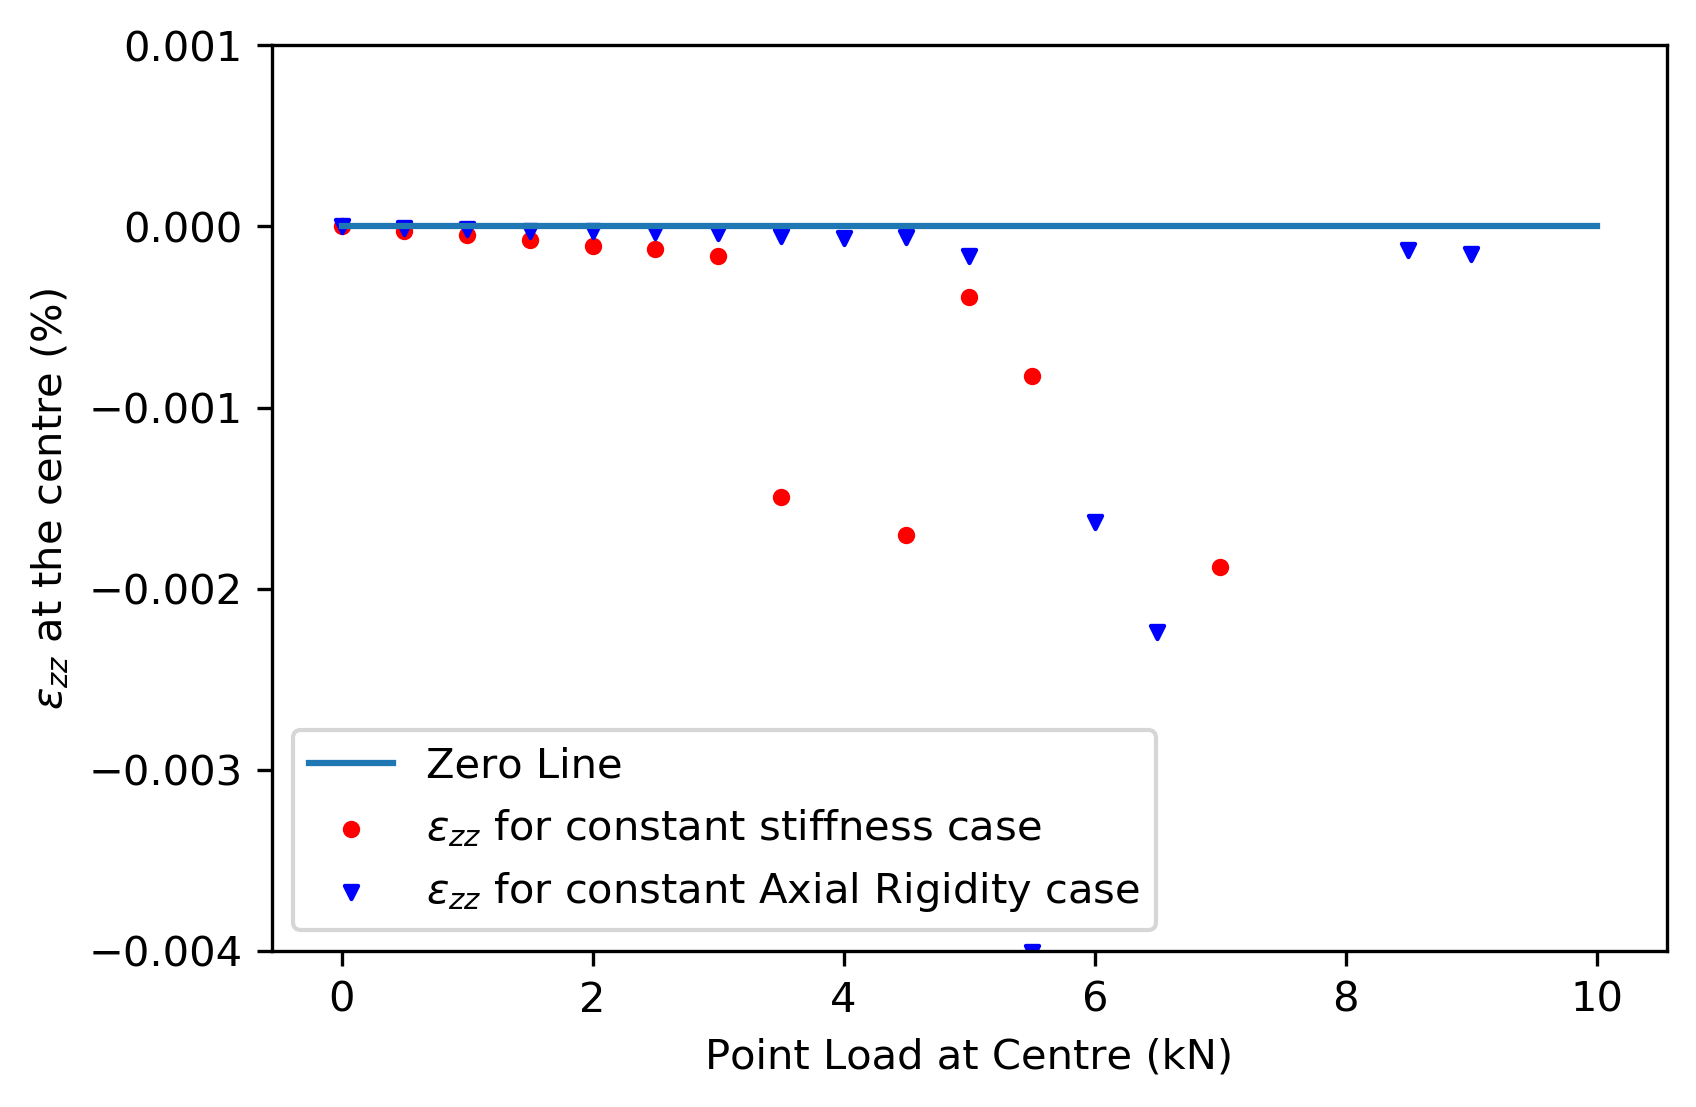
\includegraphics[width = 0.9\textwidth]{Figures/M1_b_strain.png}
    \caption{Model 1 - Type B - $\epsilon_{zz}$ with respect to Point Load at centre}
    \label{fig:M1_b_strain_plt}
\end{figure}

Type B Model follows the analytical predictions for displacement more closely as compared to Type A as evident from the fig~\ref{fig:M1_b_plt}. Among the two study cases, Constant Axial Rigidity model provides better results compared to Constant Stiffness model. The normal strain in Z-direction $\epsilon_{zz}$ obtained from the model is quite erratic for loads higher than 3 kN for constant Stiffness case and loads higher than 5.5 kN for constant Axial Rigidity case as shown in the fig~\ref{fig:M1_b_strain_plt}. Some of the points not shown in fig~\ref{fig:M1_b_strain_plt} correspond to very high strain resulting from complete crushing of the vertical springs at centre under the load as shown in fig~\ref{fig:crushed_M1_b}.


\begin{figure}[!htbp]
    \centering
    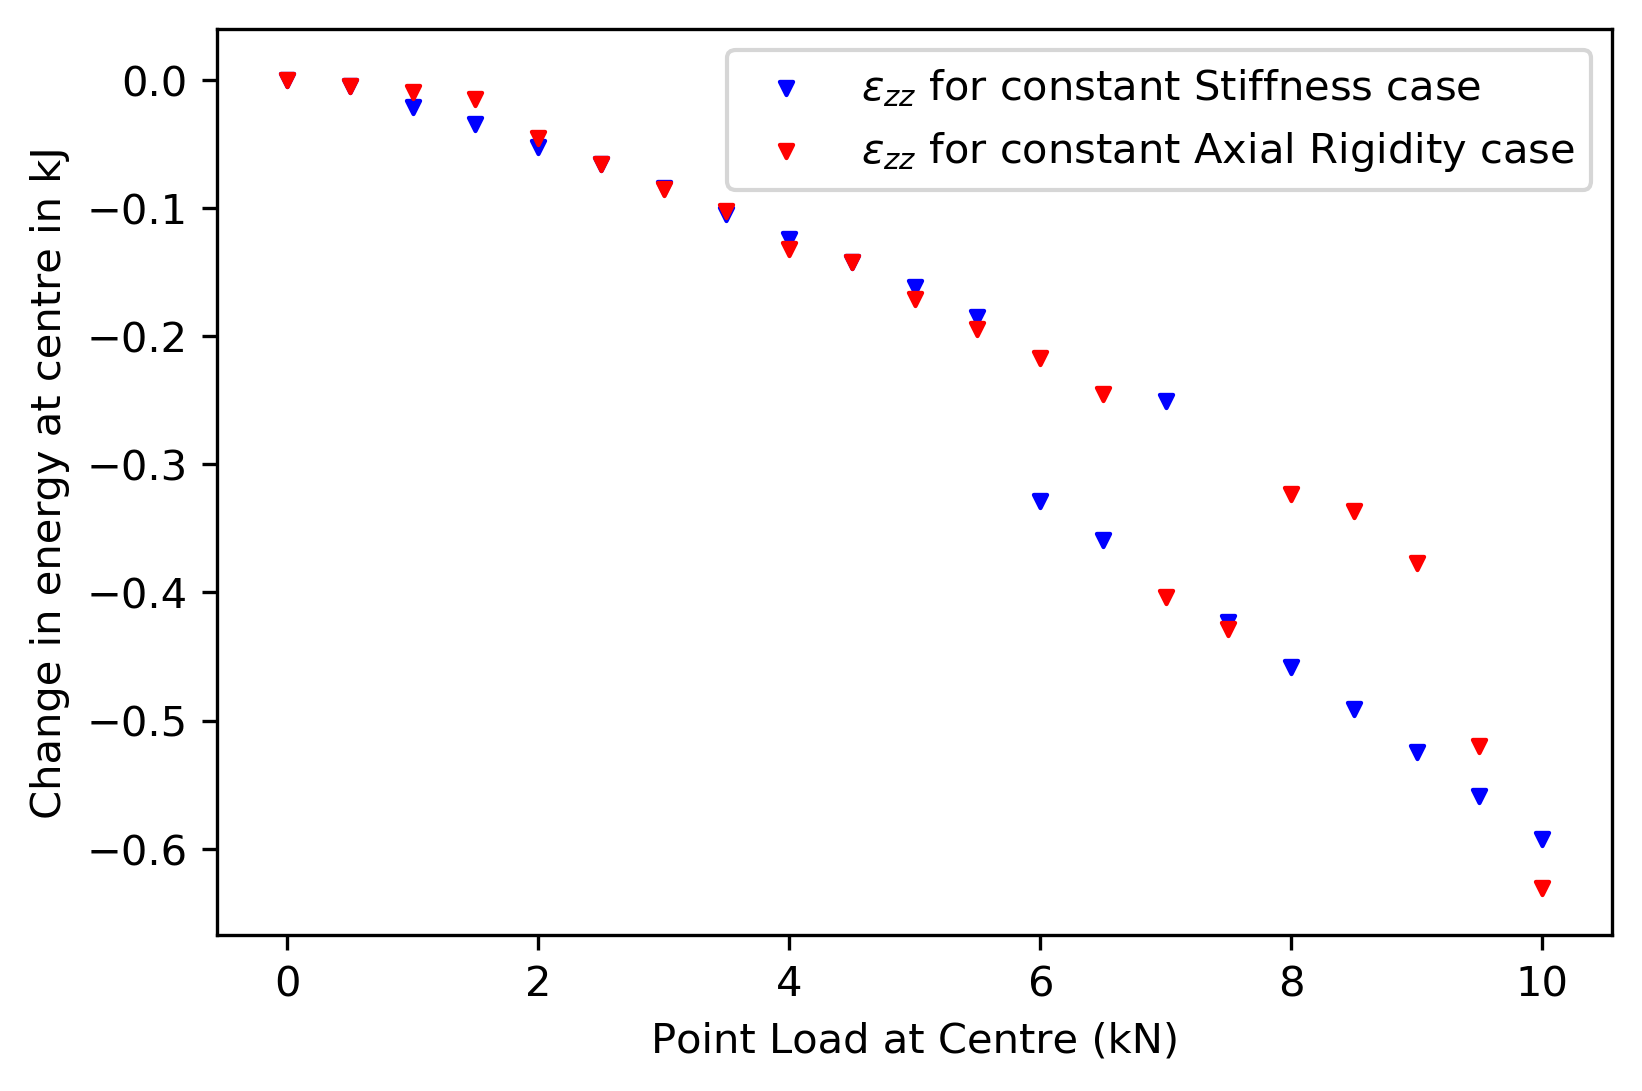
\includegraphics[width = 0.9\textwidth]{Figures/M1_b_energy.png}
    \caption{Model 1 - Type B - Change in Energy with respect to Point Load at centre}
    \label{fig:M1_b_energy}
\end{figure}

In fig~\ref{fig:M1_b_energy}, energies in the undeformed states for all forces are zero.

\begin{figure}[!htbp]
    \centering
    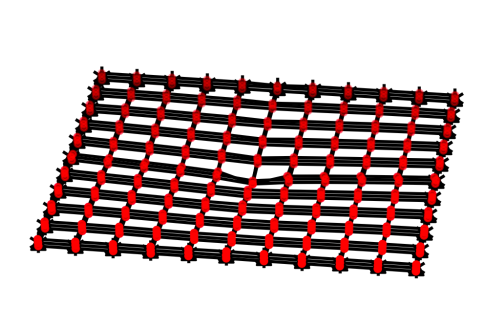
\includegraphics[width = 0.6\textwidth]{Figures/crushed_M1_b.png}
    \caption{Model 1 - Type B - Crushed vertical springs under loading of 8 kN resulting in very high $\epsilon_{zz}$}
    \label{fig:crushed_M1_b}
\end{figure}

 From fig~\ref{fig:M1_b_energy}, we can see that there is a discontinuity in energy profile for Constant Stiffness case at around load of 6 kN, Some irregularities are also present in energy variation of both the cases. Interestingly, for Constant Axial Rigidity case, the point where there is a discontinuity in energy field (around 6 kN) is the same point at which the predictions for vertical displacements start deviating from the analytical results obtained from First-order Shear Deformation theory and strains turn sporadic, even though energies after discontinuity in energy profiles are lower compared to the energies at the same loading if they continued the earlier pattern. This suggests a sharp change in the properties of the model or some kind of instability which leads to such results. 
 
 \subsubsection{Model 1 - Type C}
 Model 1 - Type C is 20 x 20 x 2 structure of Model 1 cuboids of dimensions 0.05~m x 0.05~m x 0.01~m. The model is shown in fig~\ref{fig:M1_c_XY} - fig~\ref{fig:M1_c_3D}

\begin{figure}[!htbp]
\begin{minipage}{0.3\textwidth}
    \centering
    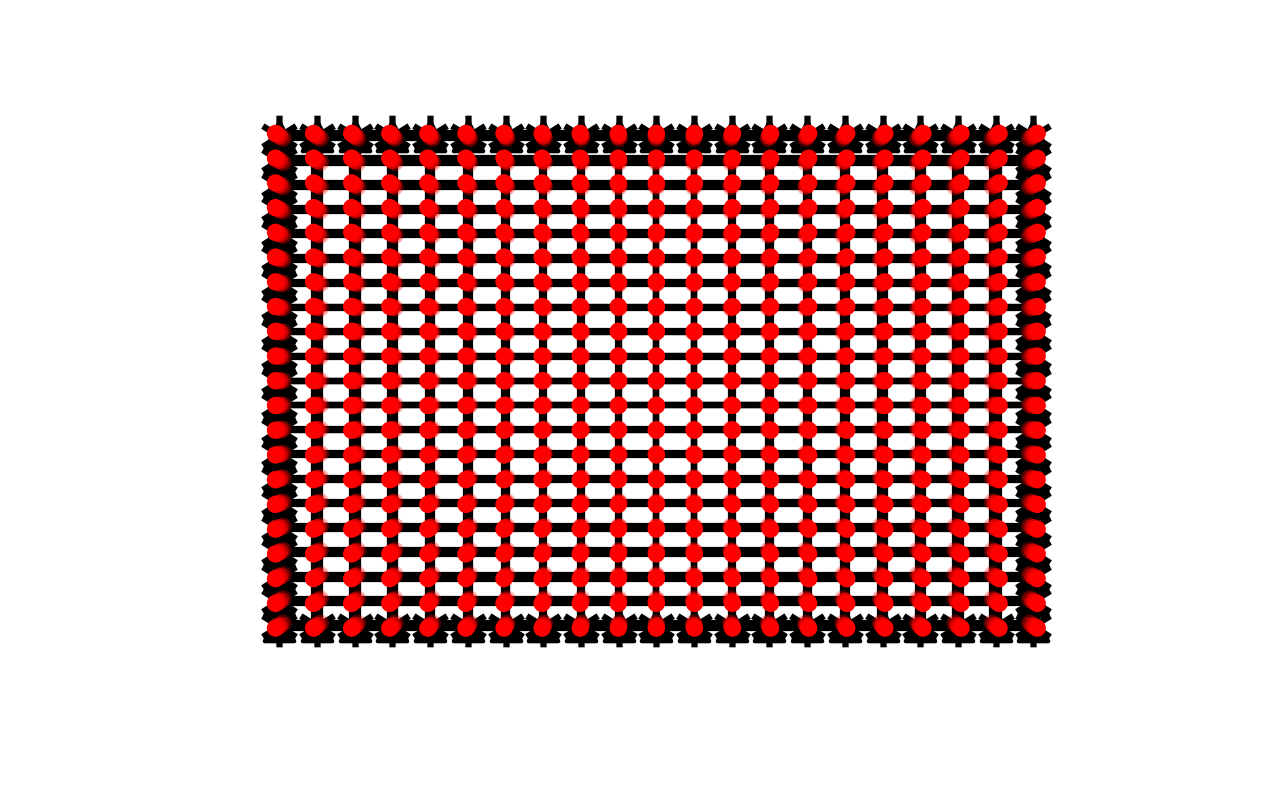
\includegraphics[width = 1\textwidth]{Figures/M1_type_c_XY.png}
    \caption{Model 1 - Type C - XY Projection}
    \label{fig:M1_c_XY}
\end{minipage}
\hspace{5mm}
\begin{minipage}{0.3\textwidth}
    \centering
    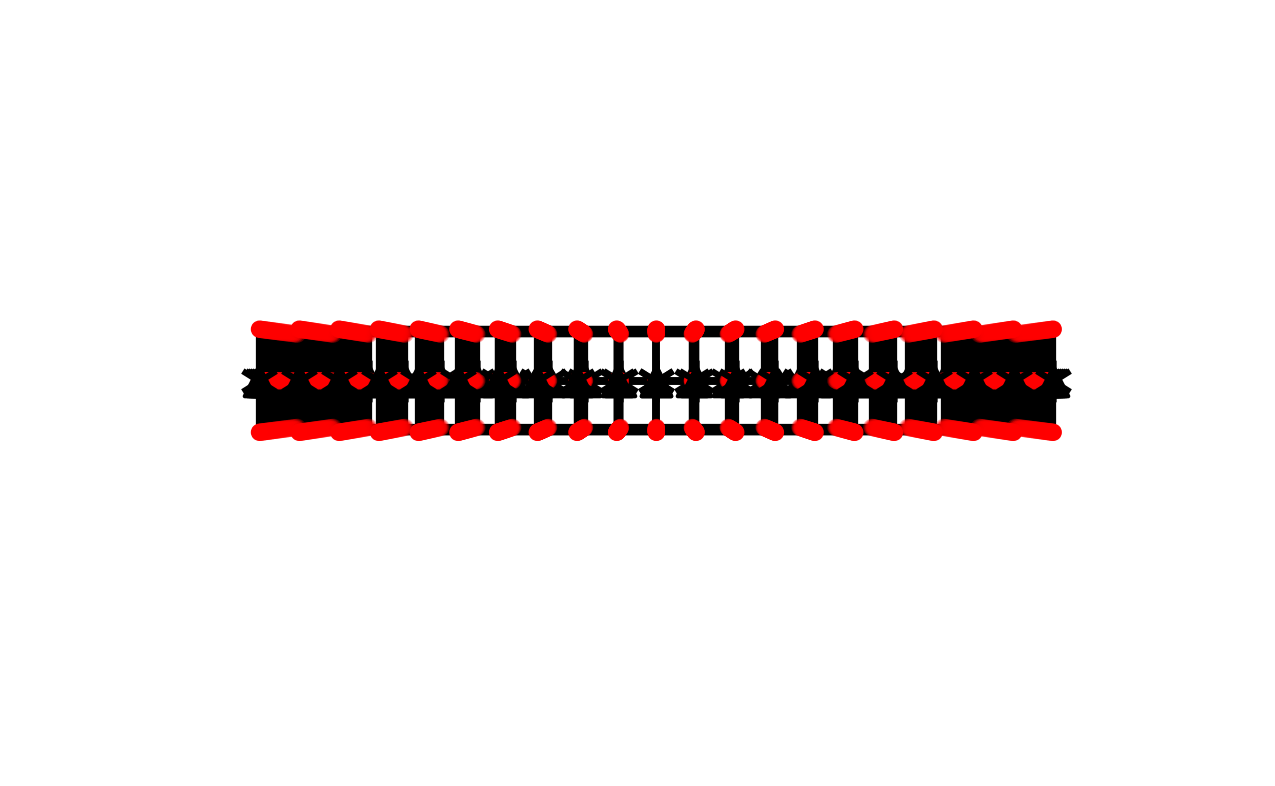
\includegraphics[width = 1\textwidth]{Figures/M1_type_c_YZ.png}
    \caption{Model 1 - Type C - YZ Projection}
    \label{fig:M1_c_YZ}
\end{minipage}
\hspace{5mm}
\begin{minipage}{0.3\textwidth}
    \centering
    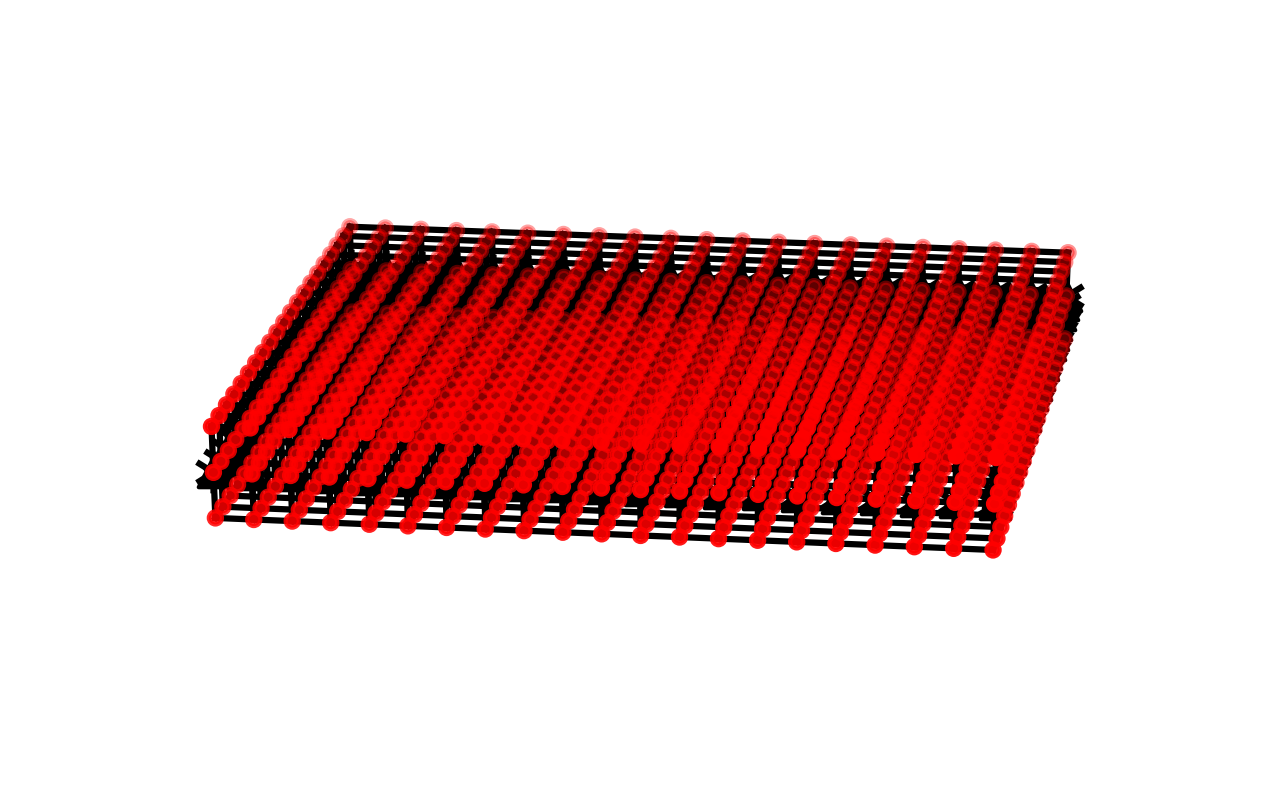
\includegraphics[width = 1\textwidth]{Figures/M1_type_c_3D.png}
    \caption{Model 1 - Type C - 3D View}
    \label{fig:M1_c_3D}
\end{minipage}
\end{figure}

The plots corresponding to Model 1 - Type C are shown in fig~\ref{fig:M1_c_plt} - fig~\ref{fig:M1_c_energy}


Model 1 - Type C predictions for vertical deflection at centre are similar to that predicted by Model 1 - Type B, however the predictions are more uniform and closely follow the analytical prediction at smaller loads. In this case both, Constant Axial Rigidity and Constant Stiffness, study predict almost similar deflection. However, unlike Model 1 - Type A and Model 1 - Type B, Constant stiffness study predicts deflection closer to analytical predictions, although marginally, compared to Constant Axial Rigidity study.

\begin{figure}[!htbp]
    \centering
    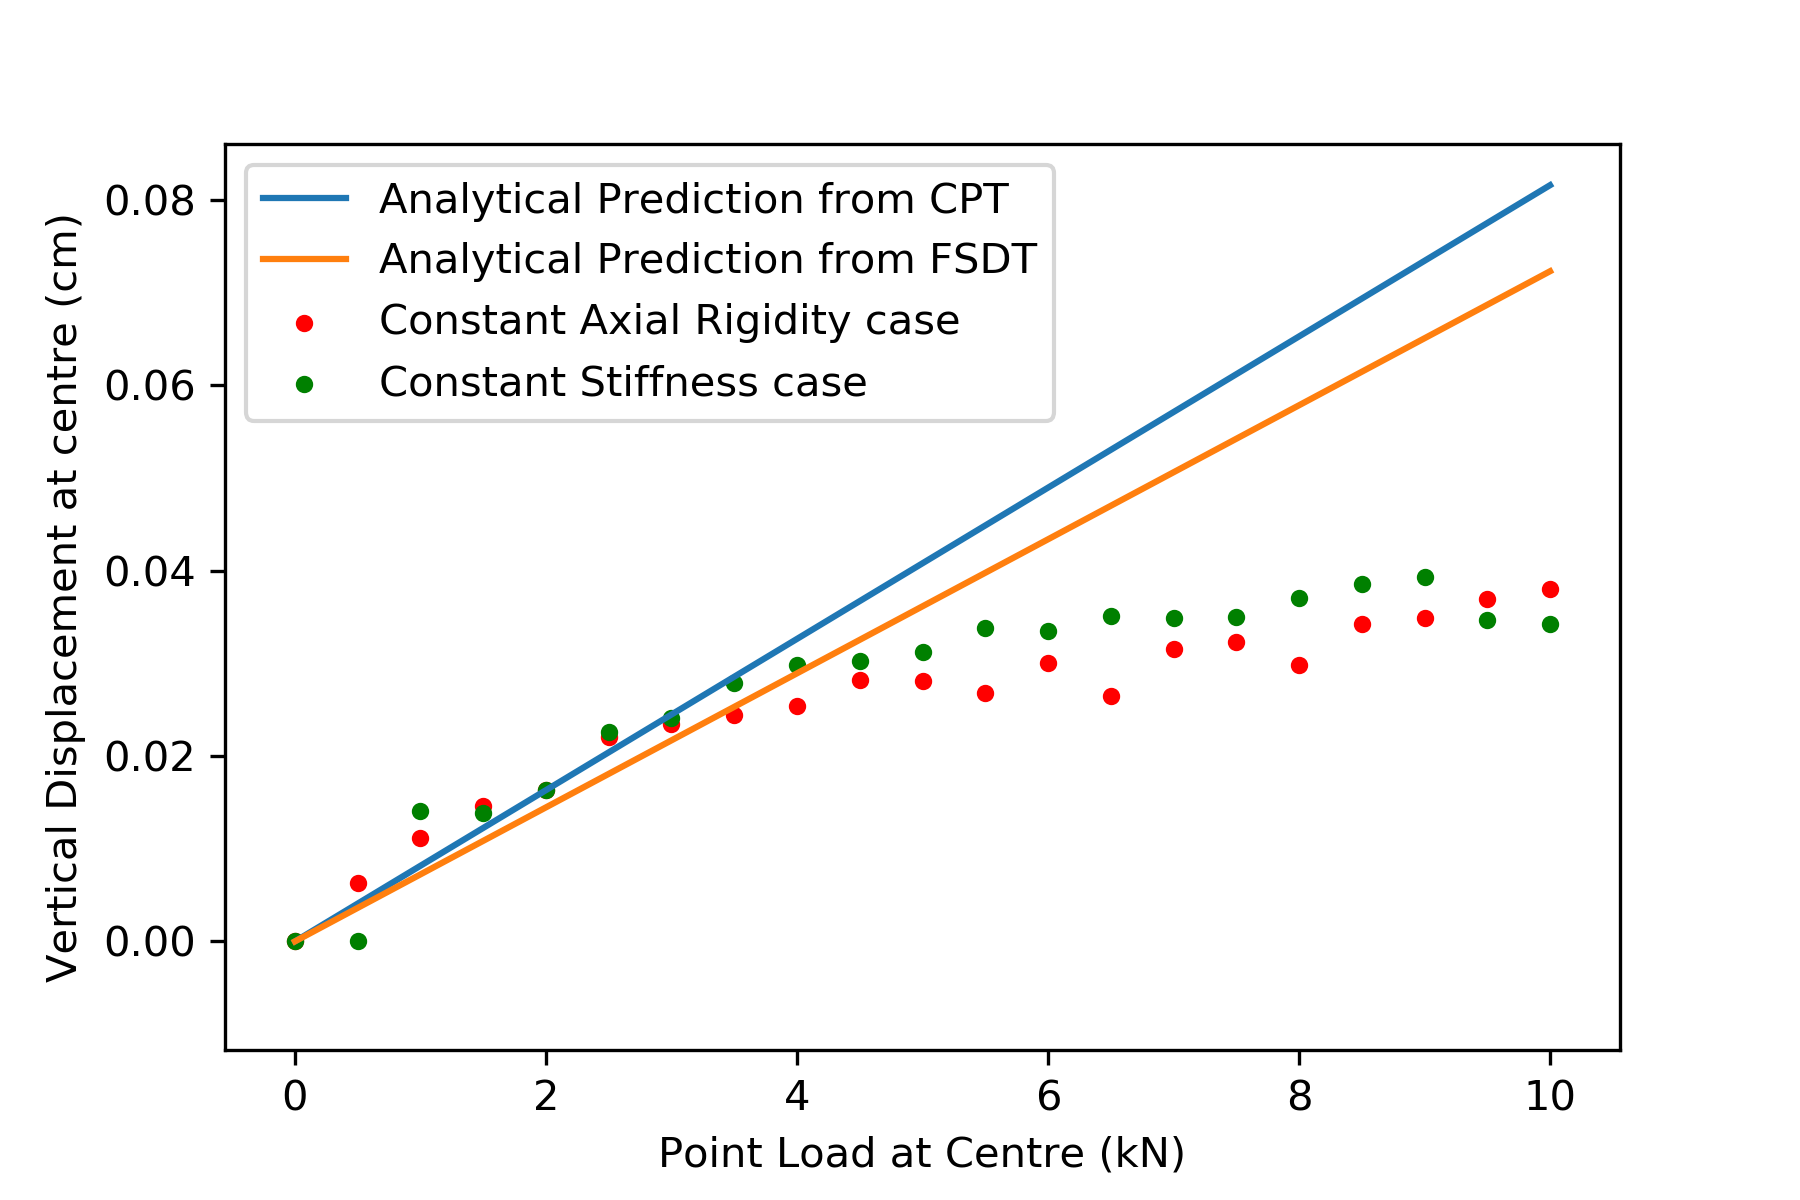
\includegraphics[width = 0.8\textwidth]{Figures/M1_c_plt.png}
    \caption{Model 1 - Type C - vertical Displacement with respect to Point Load at centre}
    \label{fig:M1_c_plt}
\end{figure}

\begin{figure}[!htbp]
    \centering
    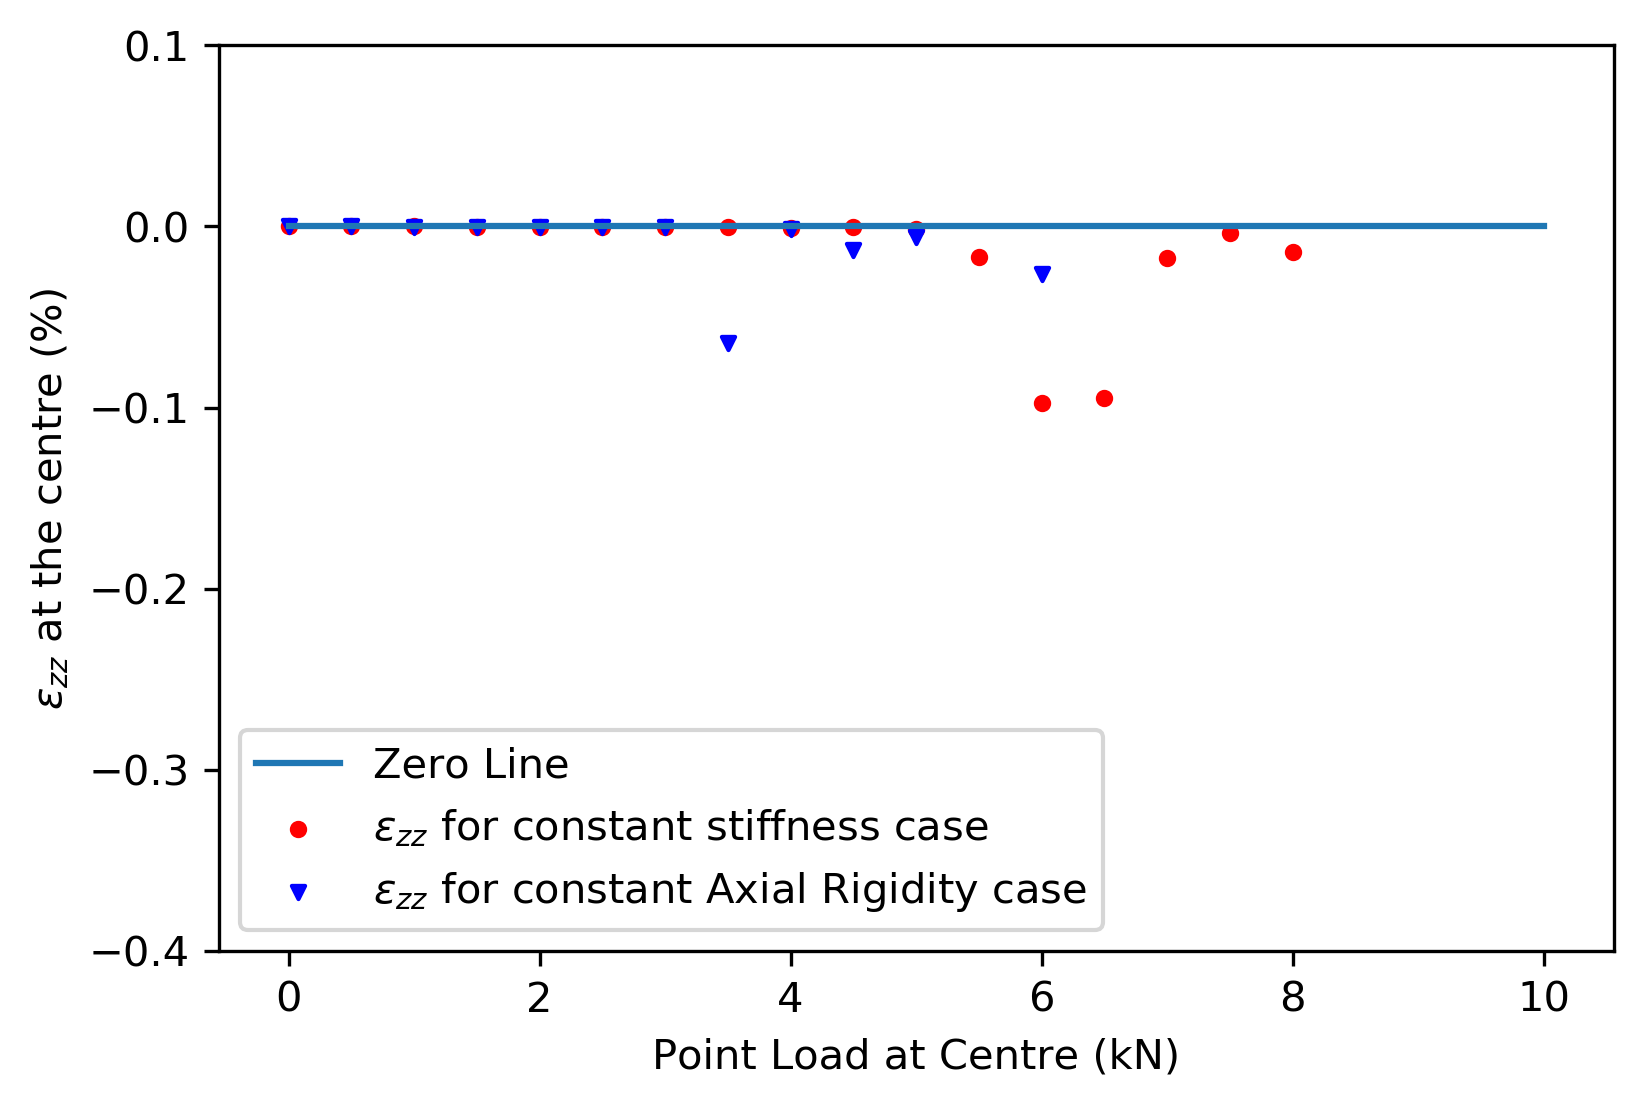
\includegraphics[width = 0.9\textwidth]{Figures/M1_c_strain.png}
    \caption{Model 1 - Type C - $\epsilon_{zz}$ with respect to Point Load at centre}
    \label{fig:M1_c_strain_plt}
\end{figure}

Strains predicted by this model are similar to those predicted by Type A and Type B models at lower load, however the vertical strains turn to be very erratic and large for higher loading. Some of the points with very high strains are not shown in the fig~\ref{fig:M1_c_strain_plt}. 

\begin{figure}[!htbp]
    \centering
    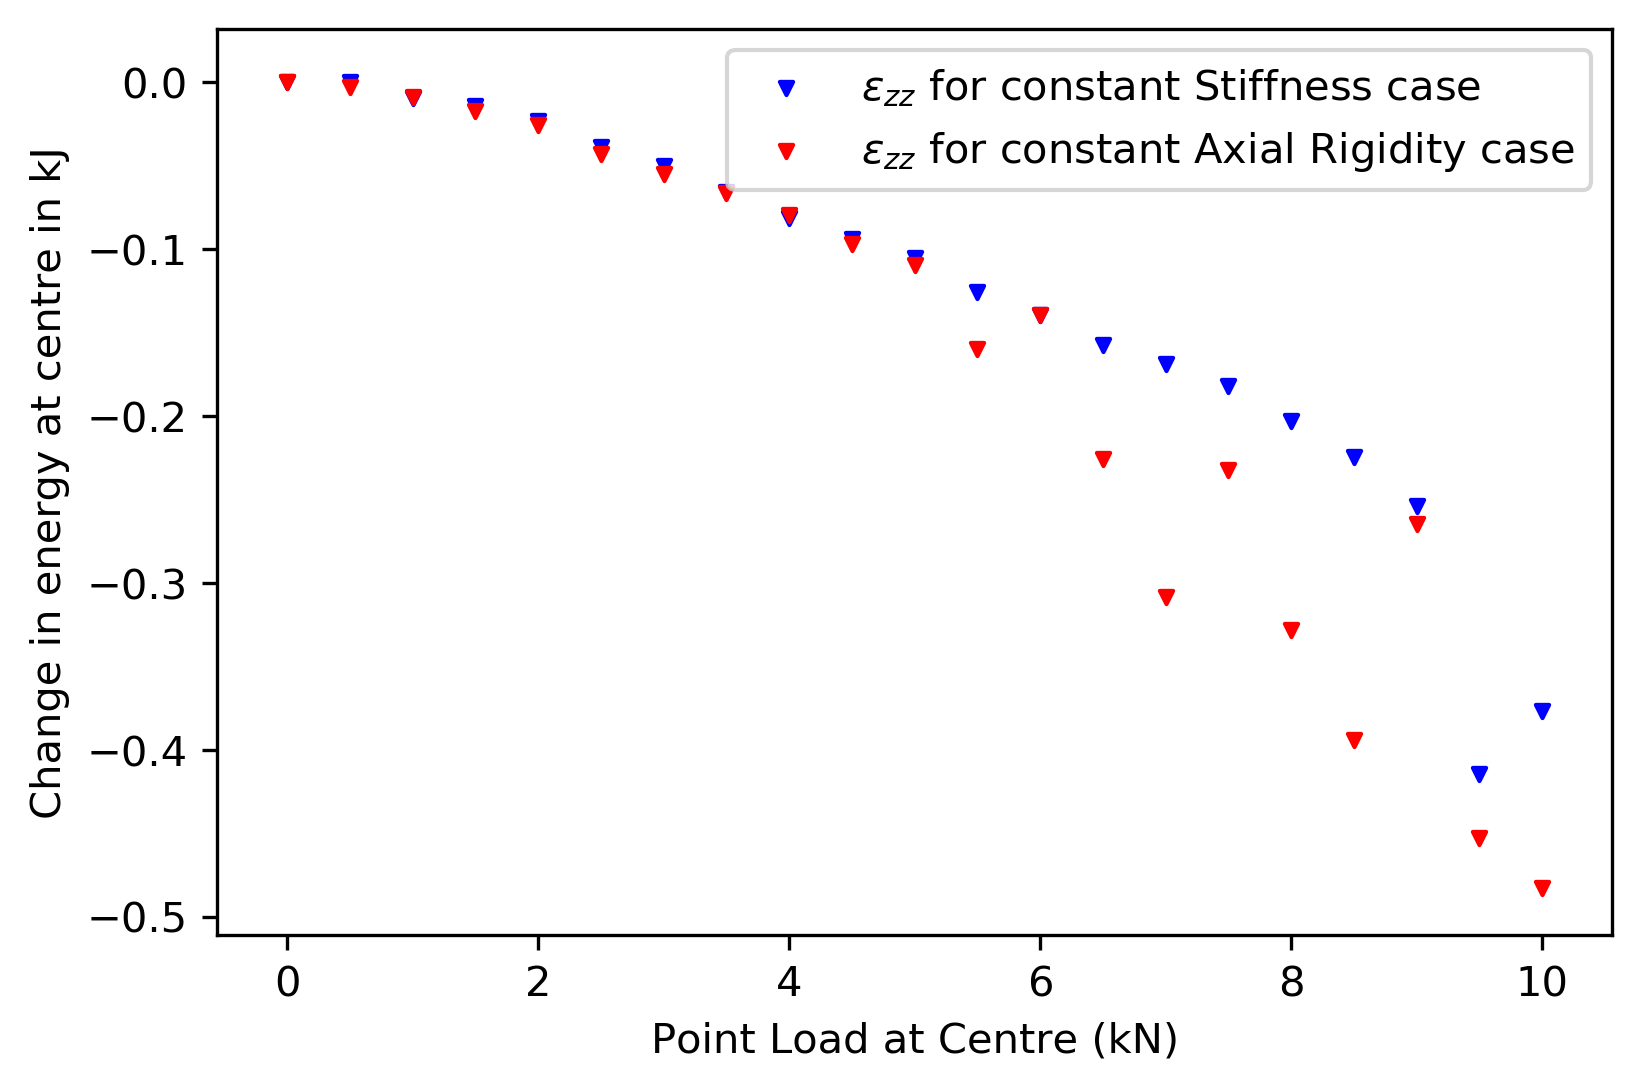
\includegraphics[width = 0.9\textwidth]{Figures/M1_c_energy.png}
    \caption{Model 1 - Type C - Change in Energy with respect to Point Load at centre}
    \label{fig:M1_c_energy}
\end{figure}

In fig~\ref{fig:M1_c_energy}, energies in the undeformed states for all forces are zero.

The energy profiles are smoother compared to the energy profiles of Type A and Type B models. The energy for Constant stiffness case at higher loading are higher than that of Constant Axial Rigidity case. Also there is a kind of oscillating pattern in the energy values obtained for Constant Axial Rigidity case for loads higher than 5 kN. 

\newpage
\subsection{Model 2}
Model 2 extends Model 1 by providing the planar layers of the Model with both in-plane bracings. Dimension of the plate is 1~m x 1~m x 0.02~m and stiffness of the springs in model are calibrated for displacement at centre for a 2 kN point load applied at centre with displacements at centre of an equivalent plate with $E = 2$ GPa and $\nu = 0.25$).

\subsubsection{Model 2 - Type A}
These models are type 2 model with 4 x 4 x 2 structure of cuboids of dimension 0.25~m x 0.25~m x 0.01~m stacked together as shown in the fig~\ref{fig:M2_a_XY} - fig~\ref{fig:M2_a_3D}.

\begin{figure}[!htbp]
\begin{minipage}{0.3\textwidth}
    \centering
    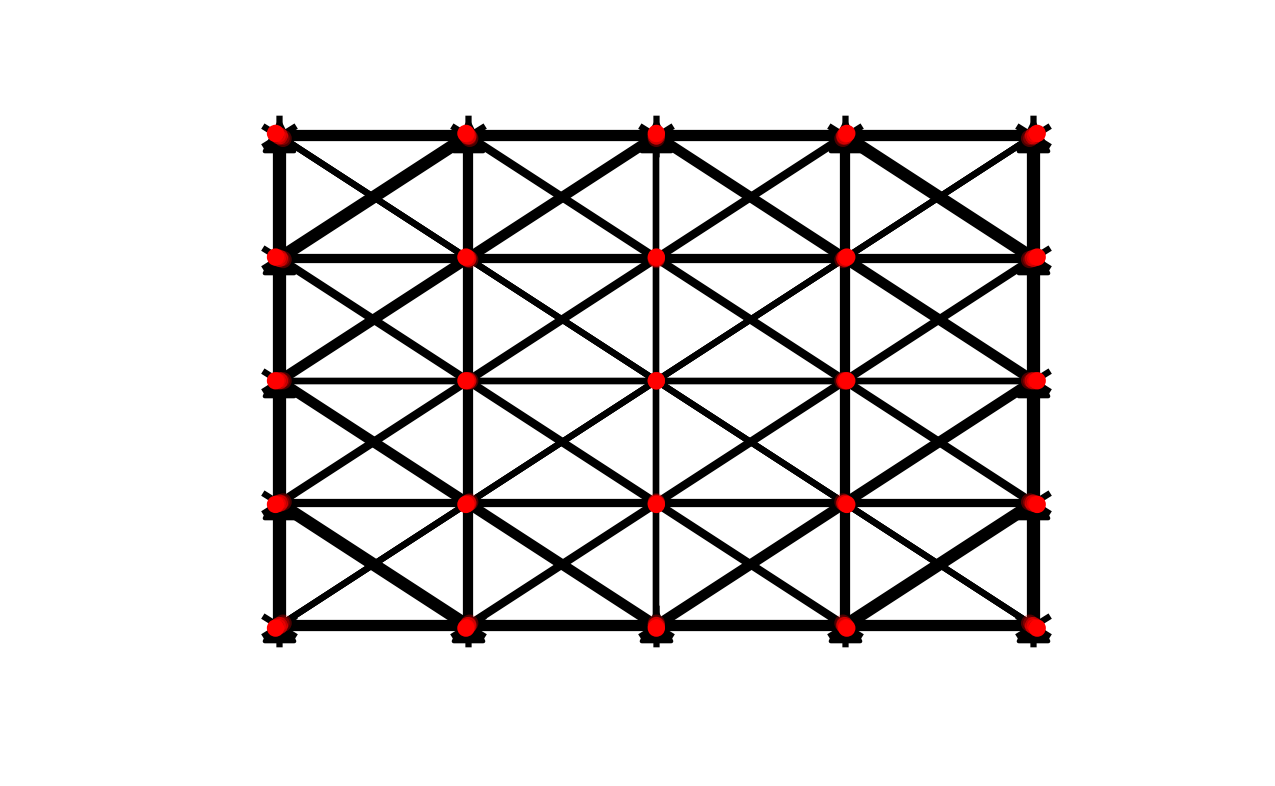
\includegraphics[width = 1\textwidth]{Figures/M2_type_a_XY.png}
    \caption{Model 2 - Type A - XY Projection}
    \label{fig:M2_a_XY}
\end{minipage}
\hspace{5mm}
\begin{minipage}{0.3\textwidth}
    \centering
    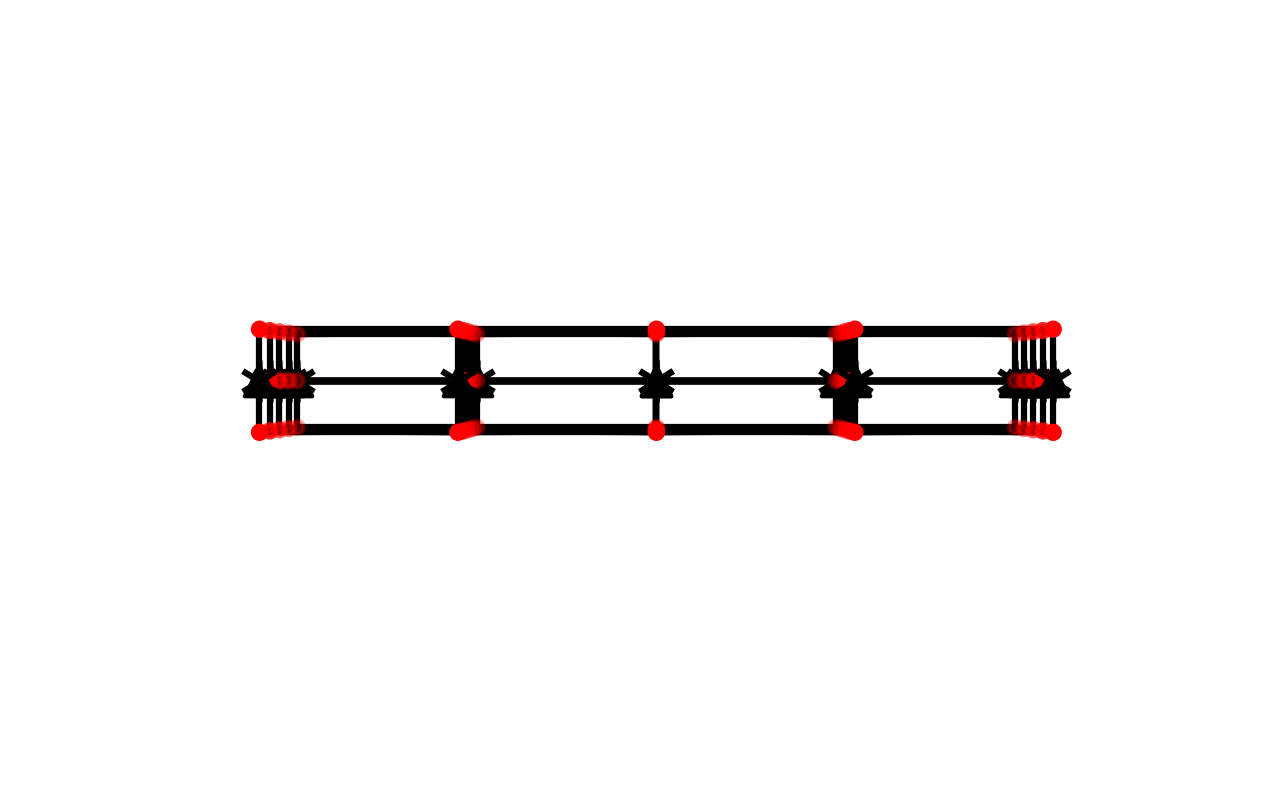
\includegraphics[width = 1\textwidth]{Figures/M2_type_a_YZ.png}
    \caption{Model 2 - Type A - YZ Projection}
    \label{fig:M2_a_YZ}
\end{minipage}
\hspace{5mm}
\begin{minipage}{0.3\textwidth}
    \centering
    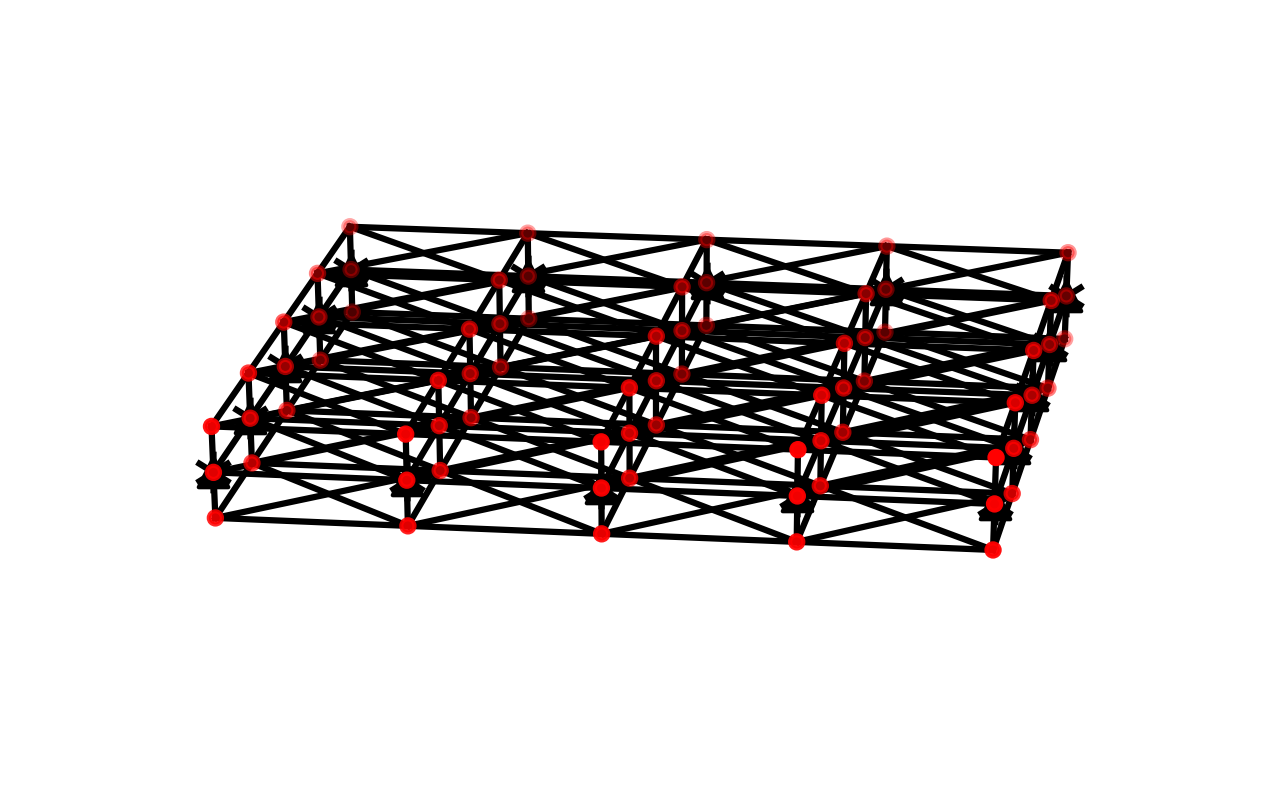
\includegraphics[width = 1\textwidth]{Figures/M2_type_a_3D.png}
    \caption{Model 2 - Type A - 3D View}
    \label{fig:M2_a_3D}
\end{minipage}
\end{figure}

The fig~\ref{fig:M2_a_plt} presents the plots for vertical deflections at centre with respect to point load applied at the centre for Constant Stiffness and Constant Axial rigidity cases.

\begin{figure}[!htbp]
    \centering
    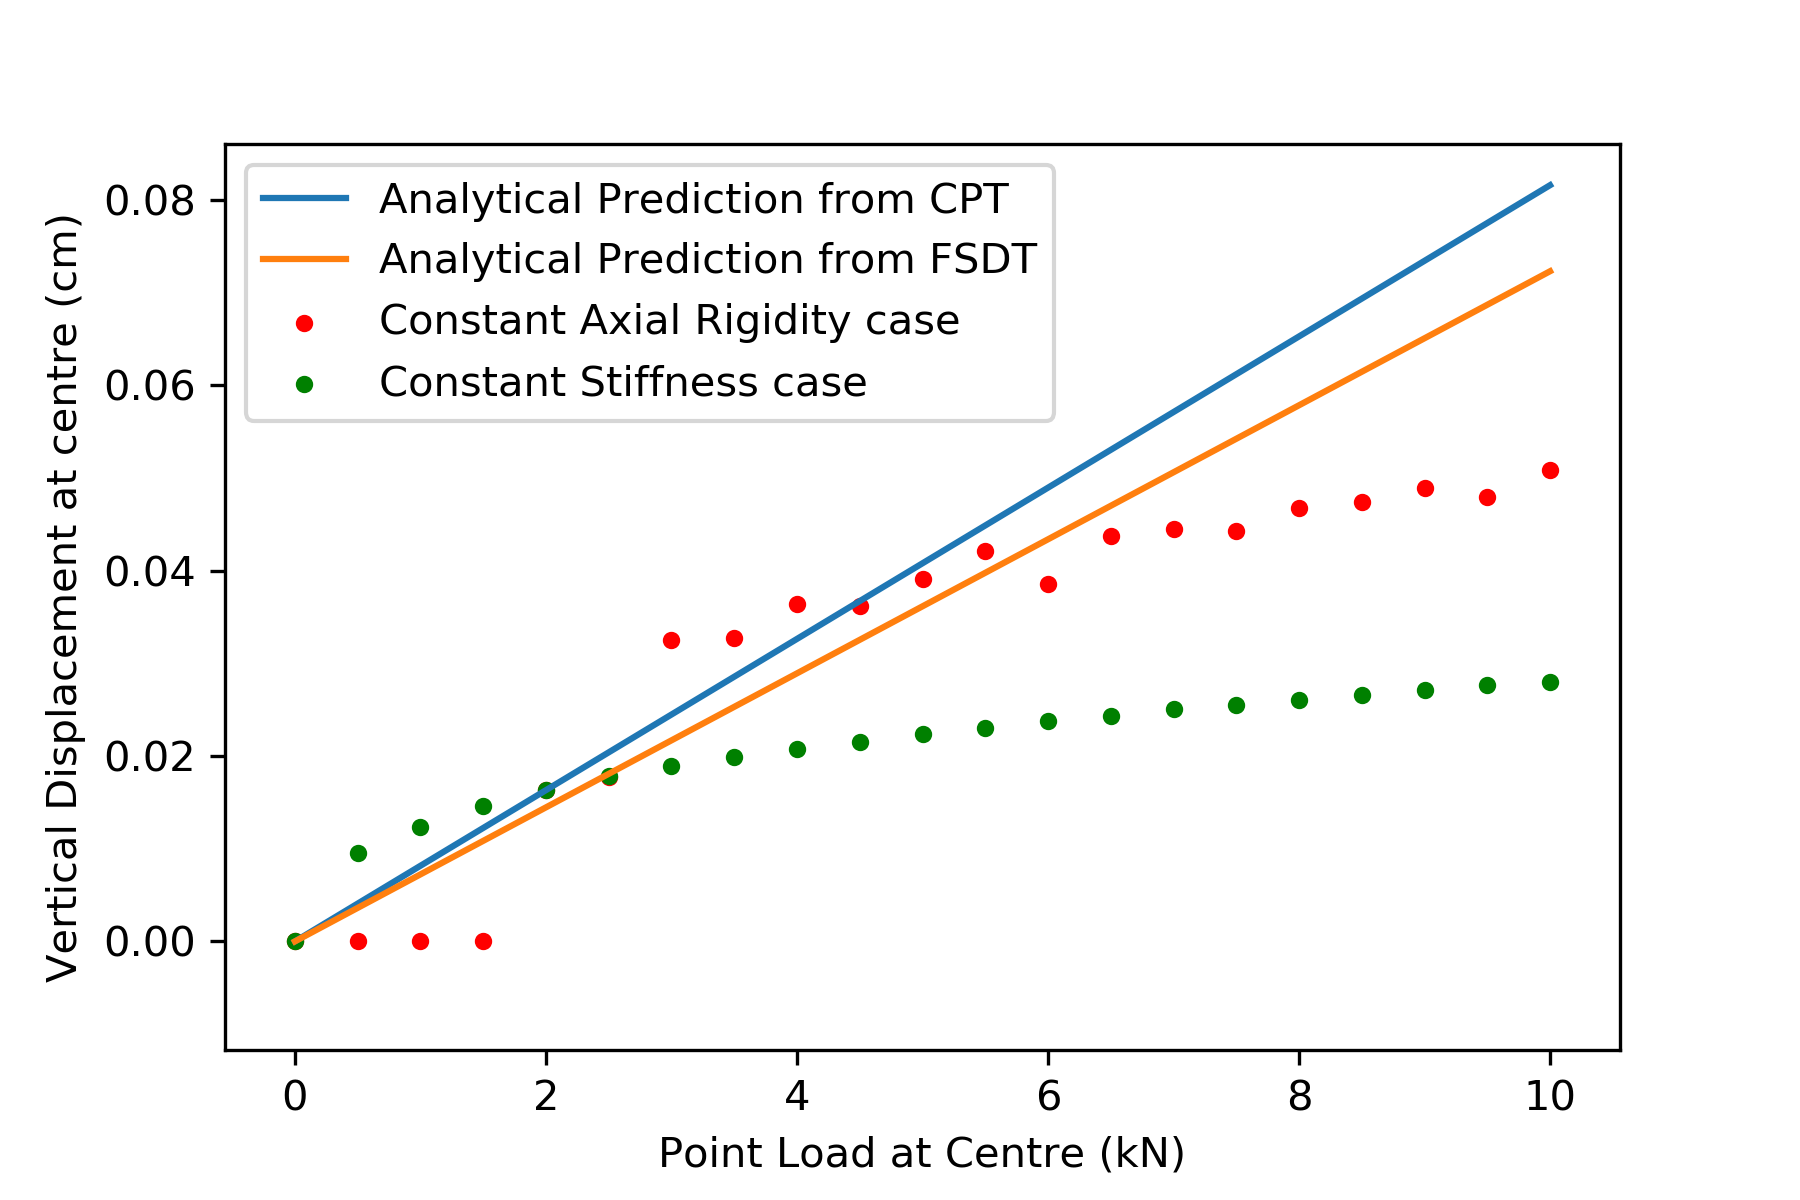
\includegraphics[width = 0.8\textwidth]{Figures/M2_a_plt.png}
    \caption{Model 2 - Type A - vertical Displacement with respect to Point Load at centre}
    \label{fig:M2_a_plt}
\end{figure}

\begin{figure}[!htbp]
    \centering
    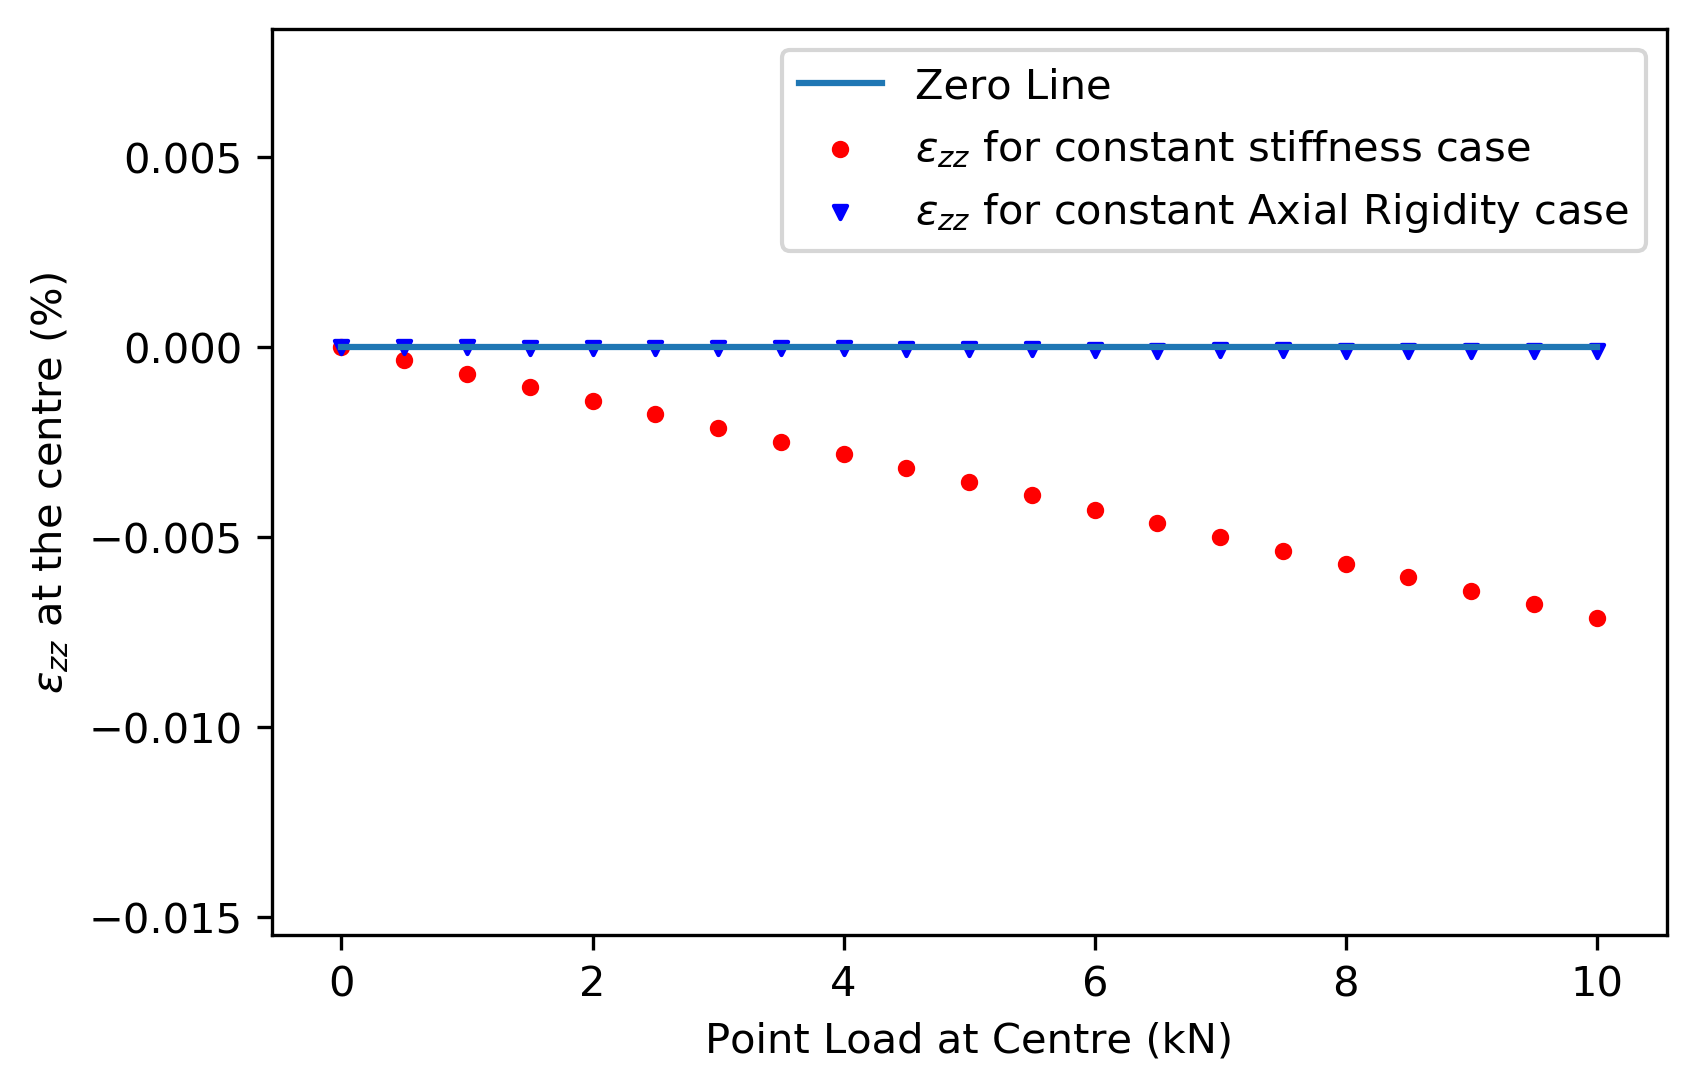
\includegraphics[width = 0.9\textwidth]{Figures/M2_a_strain.png}
    \caption{Model 2 - Type A - $\epsilon_{zz}$ with respect to Point Load at centre}
    \label{fig:M2_a_strain_plt}
\end{figure}

As evident from fig~\ref{fig:M2_a_plt}, the predictions for Constant Stiffness case, although smooth, assume a parabolic shape and achieve a plateau. They start behaving as a plate with very high stiffness at load of around 2 kN. In the case of Constant Axial Rigidity, the prediction of displacement is fragmented. Deflections at low load are zero due to ill conditioned matrices, underestimating the stiffness of plate for vertical deflection predictions then quickly rise above analytical values at a loading of around 3 kN, and finally overestimating the stiffness reaches below analytical values for higher loads. The predictions from Constant Axial Rigidity study lie closer to the analytical solution for higher loads. More close to the analytical solution from First-order Shear Deformation theory compared to Classical Plate theory.

The deviations from analytical values for Constant stiffness case can partly be explained using fig~\ref{fig:M2_a_strain_plt}. As it can be clearly seen that vertical strain is constantly increasing and the plat is being squished at the centre, this violates the assumption $\epsilon_{zz} = 0$ (eq~\ref{eq:CPT_strains_last} and eq~\ref{eq:strain_z_FSDT}). This reduces the deflection as vertical spring absorb some of the vertical deformations and as a result the Constant Stiffness study underpredicts the vertical deflection. Nonlinear behavior of the horizontal springs under action of vertical is also responsible for deviation from analytical values in two studies.

\begin{figure}[!htbp]
    \centering
    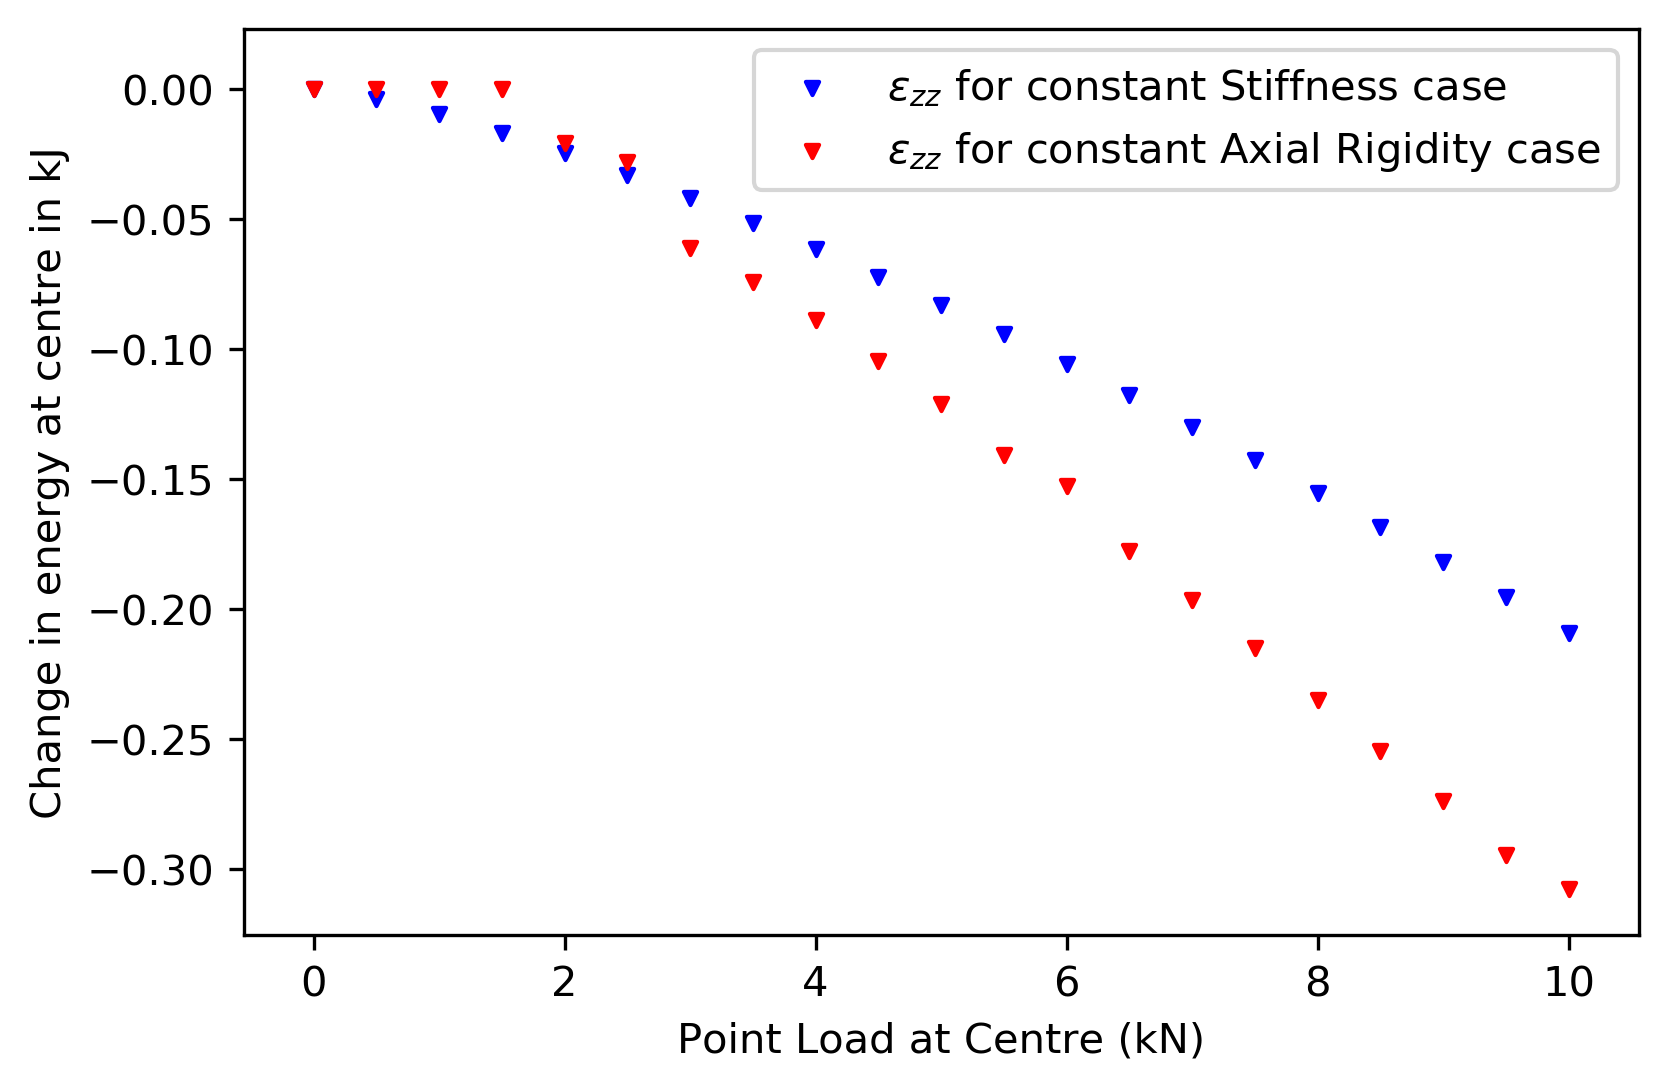
\includegraphics[width = 0.9\textwidth]{Figures/M2_a_energy.png}
    \caption{Model 2 - Type A - Change in Energy with respect to Point Load at centre}
    \label{fig:M2_a_energy}
\end{figure}

In fig~\ref{fig:M2_a_energy}, energies in the undeformed state for all forces are zero. Energy profile for Model 2 - Type A is smooth and is uniformly decreasing with force. The deflection is inversely related to the energy as it can be seen from fig~\ref{fig:M2_a_plt}. Constant Axial Rigidity model initially has higher energy than Constant stiffness case initially and as a result the deflections are lower than those predicted by Constant Stiffness Model. The energies Constant Axial Rigidity case soon drop below the energies from Constant Stiffness case and hence the deflection predicted by Axial Rigidity case are higher than Constant Stiffness case.

\subsubsection{Model 2 - Type B}
Model 2 - Type B is 10 x 10 x 2 structure of Model 2 cuboids of dimensions 0.1~m x 0.1~m x 0.01~m. The model is shown in fig~\ref{fig:M2_b_XY} - fig~\ref{fig:M2_b_3D}

\begin{figure}[!htbp]
\begin{minipage}{0.3\textwidth}
    \centering
    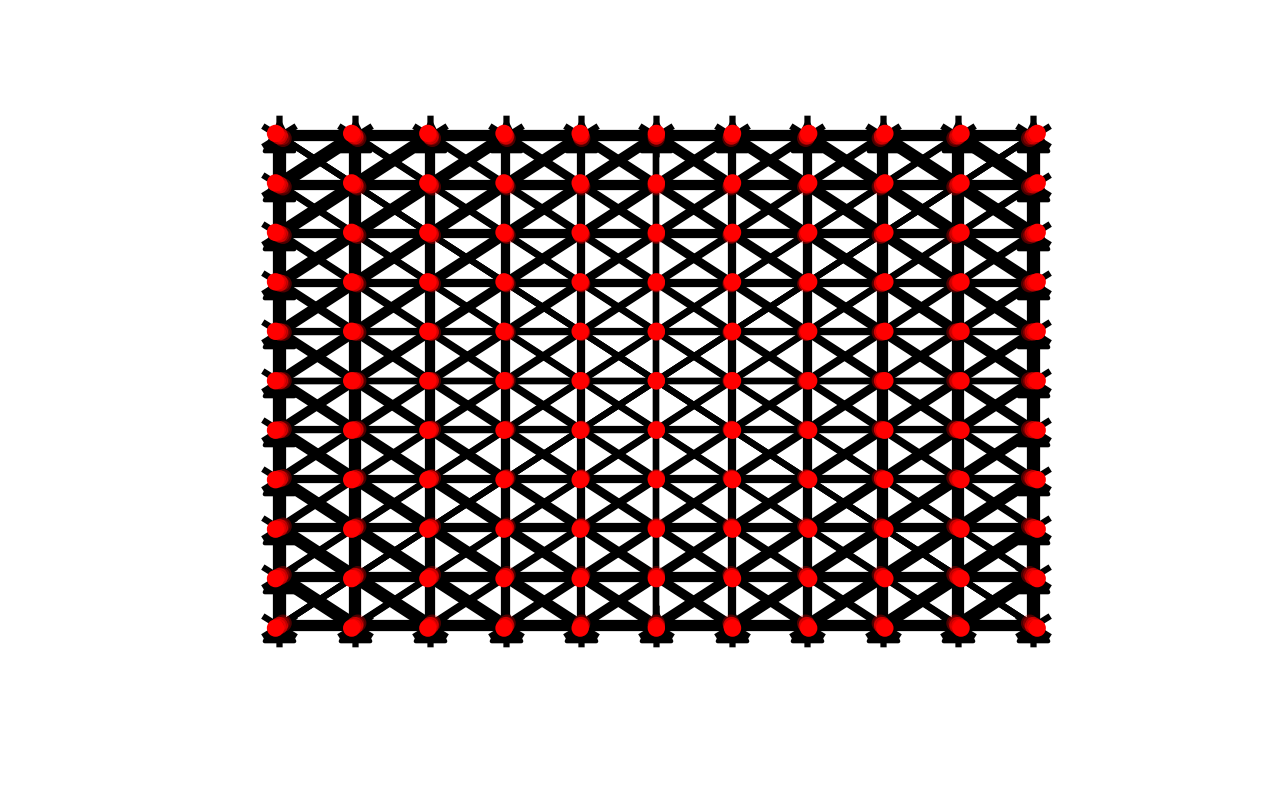
\includegraphics[width = 1\textwidth]{Figures/M2_b_XY.png}
    \caption{Model 2 - Type B - XY Projection}
    \label{fig:M2_b_XY}
\end{minipage}
\hspace{5mm}
\begin{minipage}{0.3\textwidth}
    \centering
    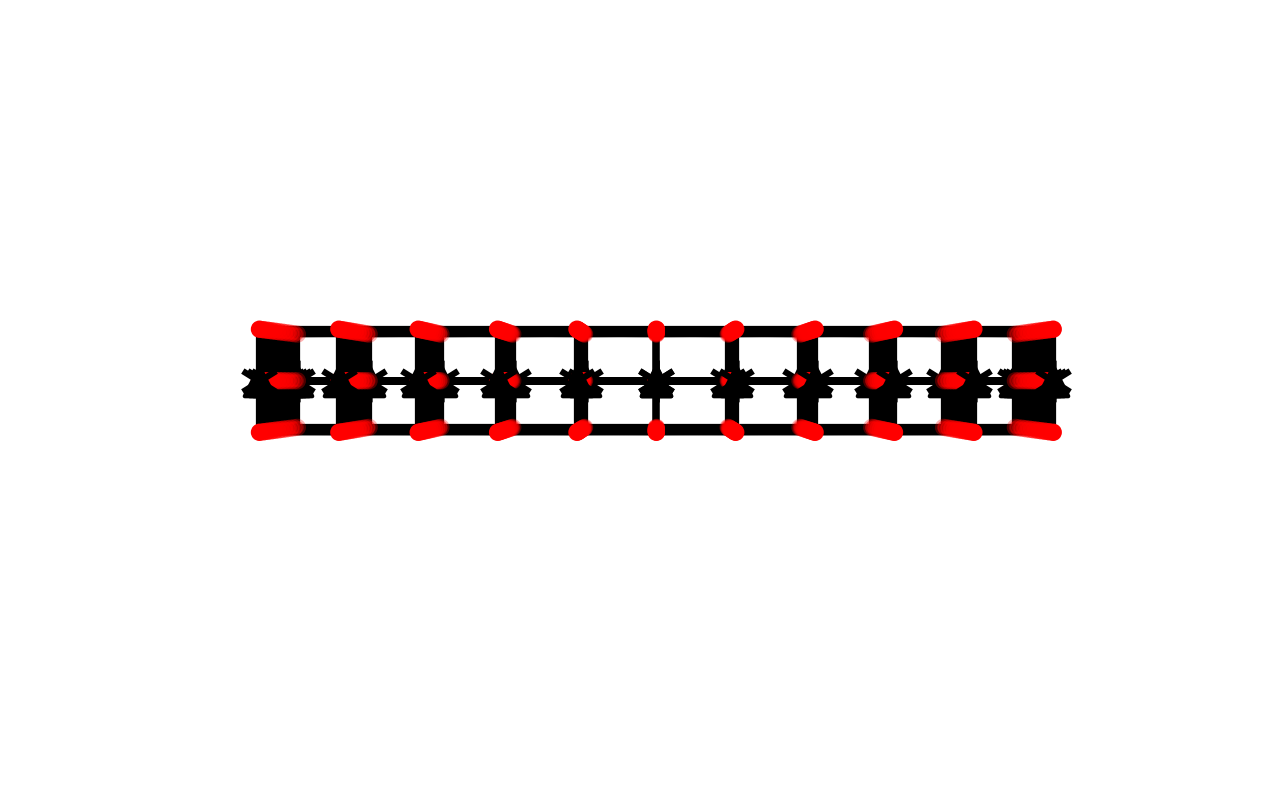
\includegraphics[width = 1\textwidth]{Figures/M2_b_YZ.png}
    \caption{Model 2 - Type B - YZ Projection}
    \label{fig:M2_b_YZ}
\end{minipage}
\hspace{5mm}
\begin{minipage}{0.3\textwidth}
    \centering
    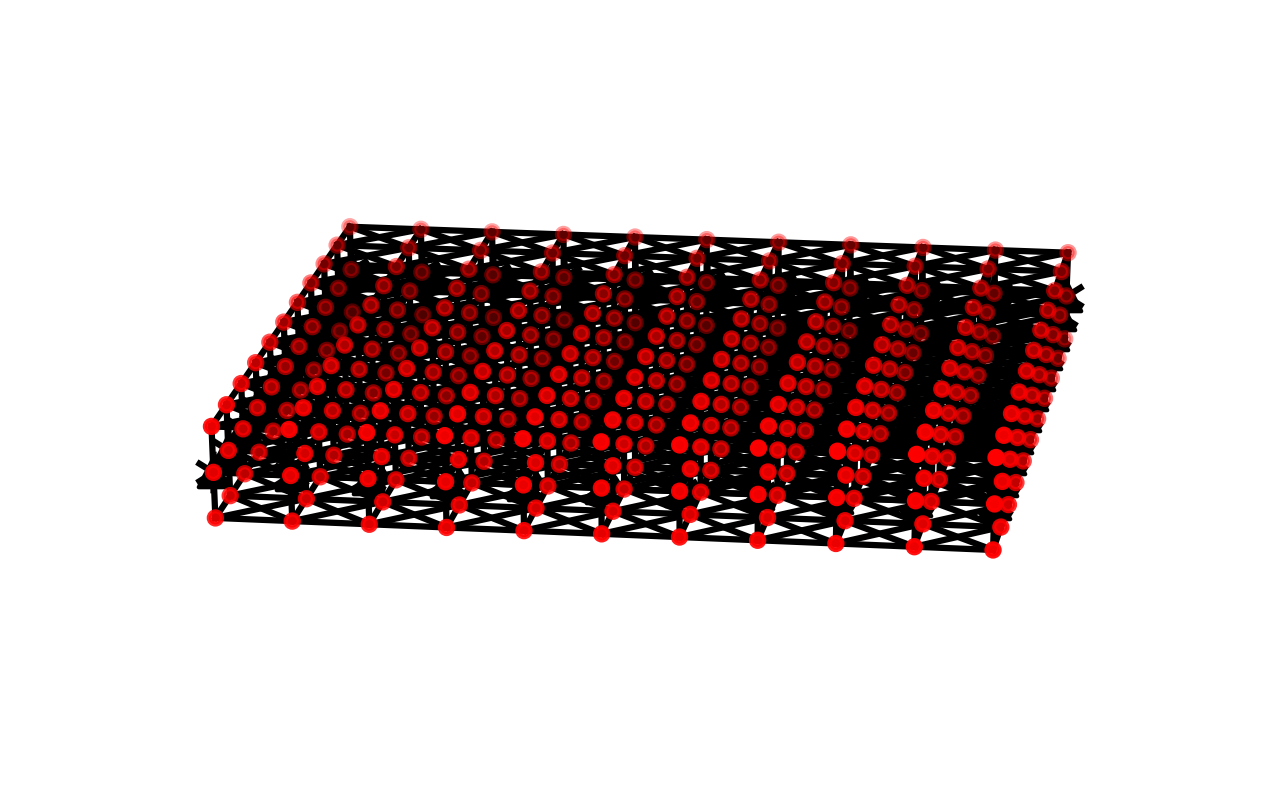
\includegraphics[width = 1\textwidth]{Figures/M2_b_3D.png}
    \caption{Model 2 - Type B - 3D View}
    \label{fig:M2_b_3D}
\end{minipage}
\end{figure}

The plots corresponding to Model 2 - Type B are shown in fig~\ref{fig:M2_b_plt} - fig~\ref{fig:M2_b_energy}. The deflection predictions for Constant Stiffness case assumes a parabolic shape similar to that in Model 2 - Type A. However, in Type B model, the predictions from Constant Axial Rigidity model closely follow the predictions from Constant Stiffness model, although this results in larger deviation from analytical results. The deviation of the prediction can again be explained through the combination of violation of the assumption $\epsilon_{zz} = 0$ and non-linear behavior of horizontal spring system under vertical loading as discussed in Model 2 - Type A section. The inverse relation between energy and deflection discussed in Model 2 - Type A section also holds.

\begin{figure}[!htbp]
    \centering
    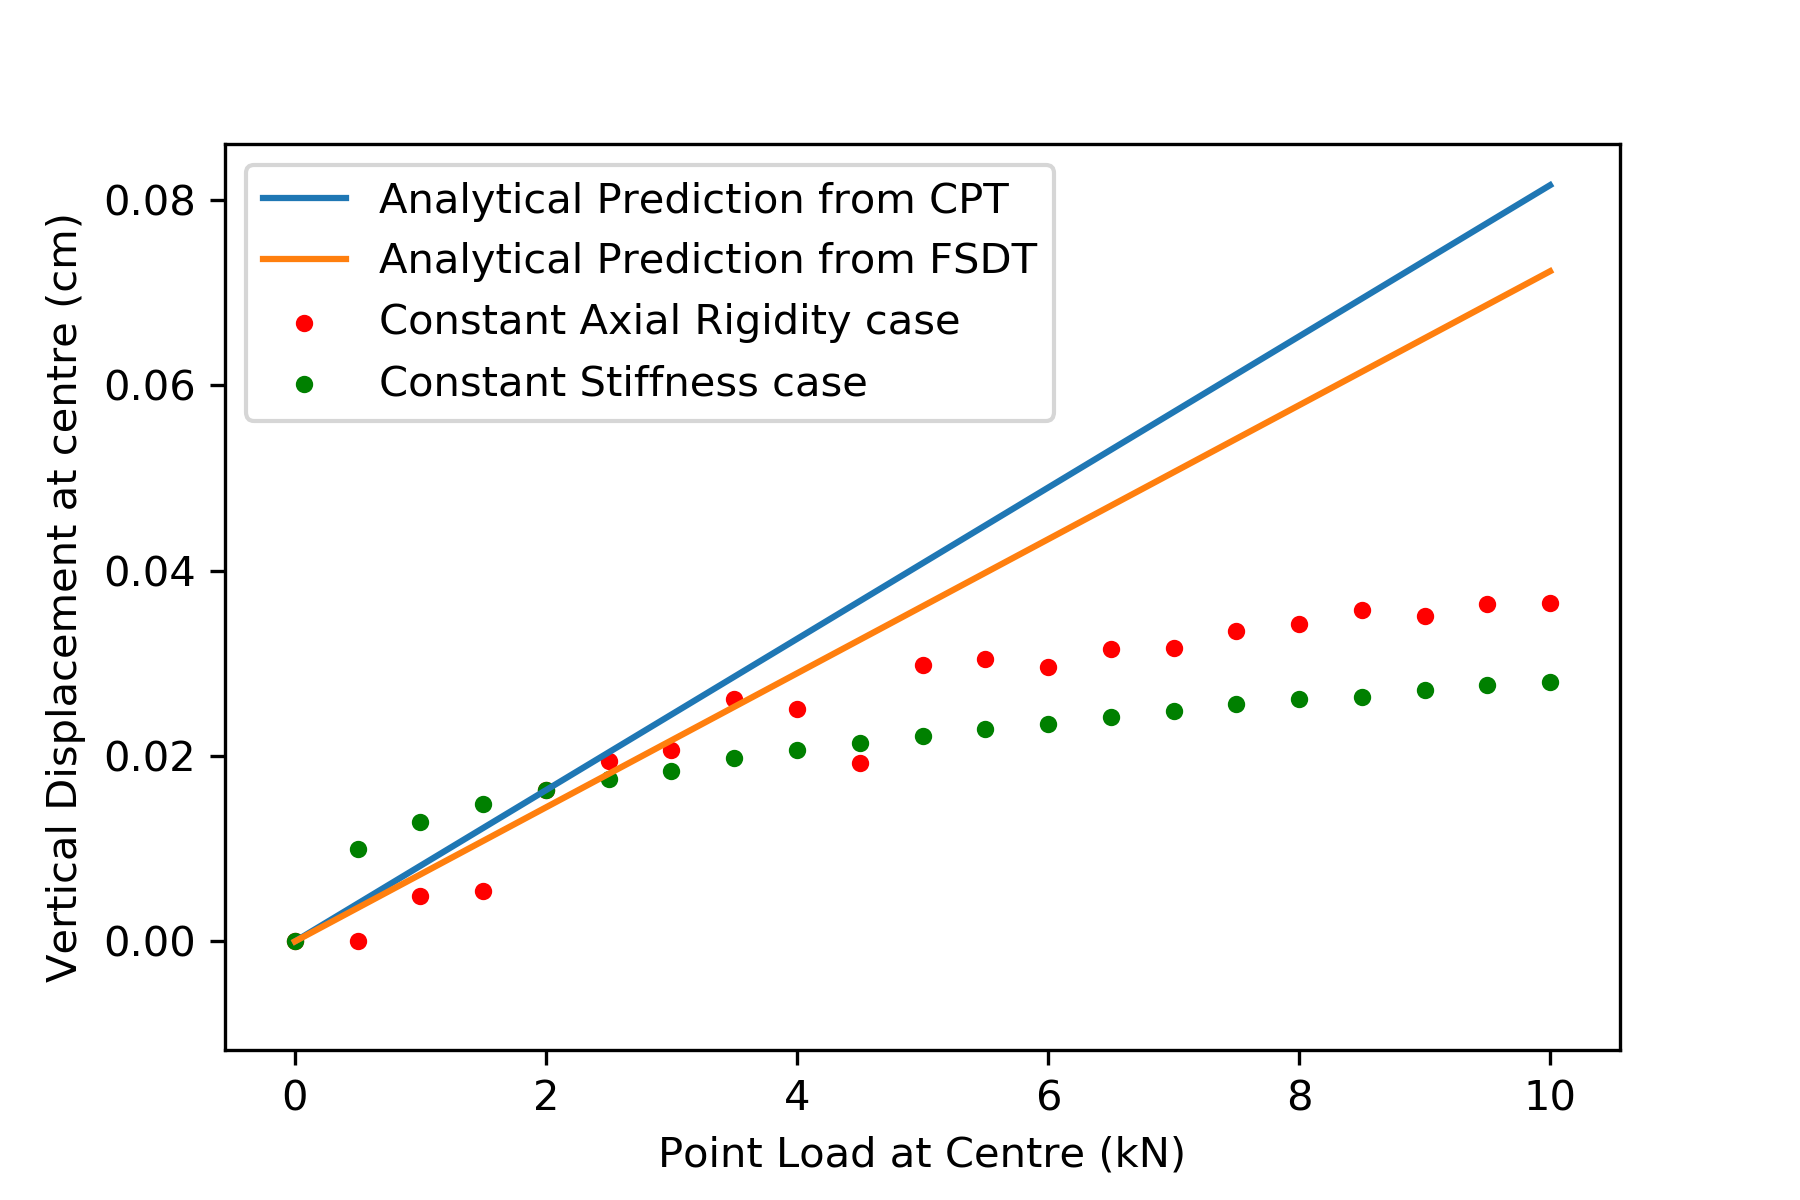
\includegraphics[width = 0.8\textwidth]{Figures/M2_b_plt.png}
    \caption{Model 2 - Type B - vertical Displacement with respect to Point Load at centre}
    \label{fig:M2_b_plt}
\end{figure}

\begin{figure}[!htbp]
    \centering
    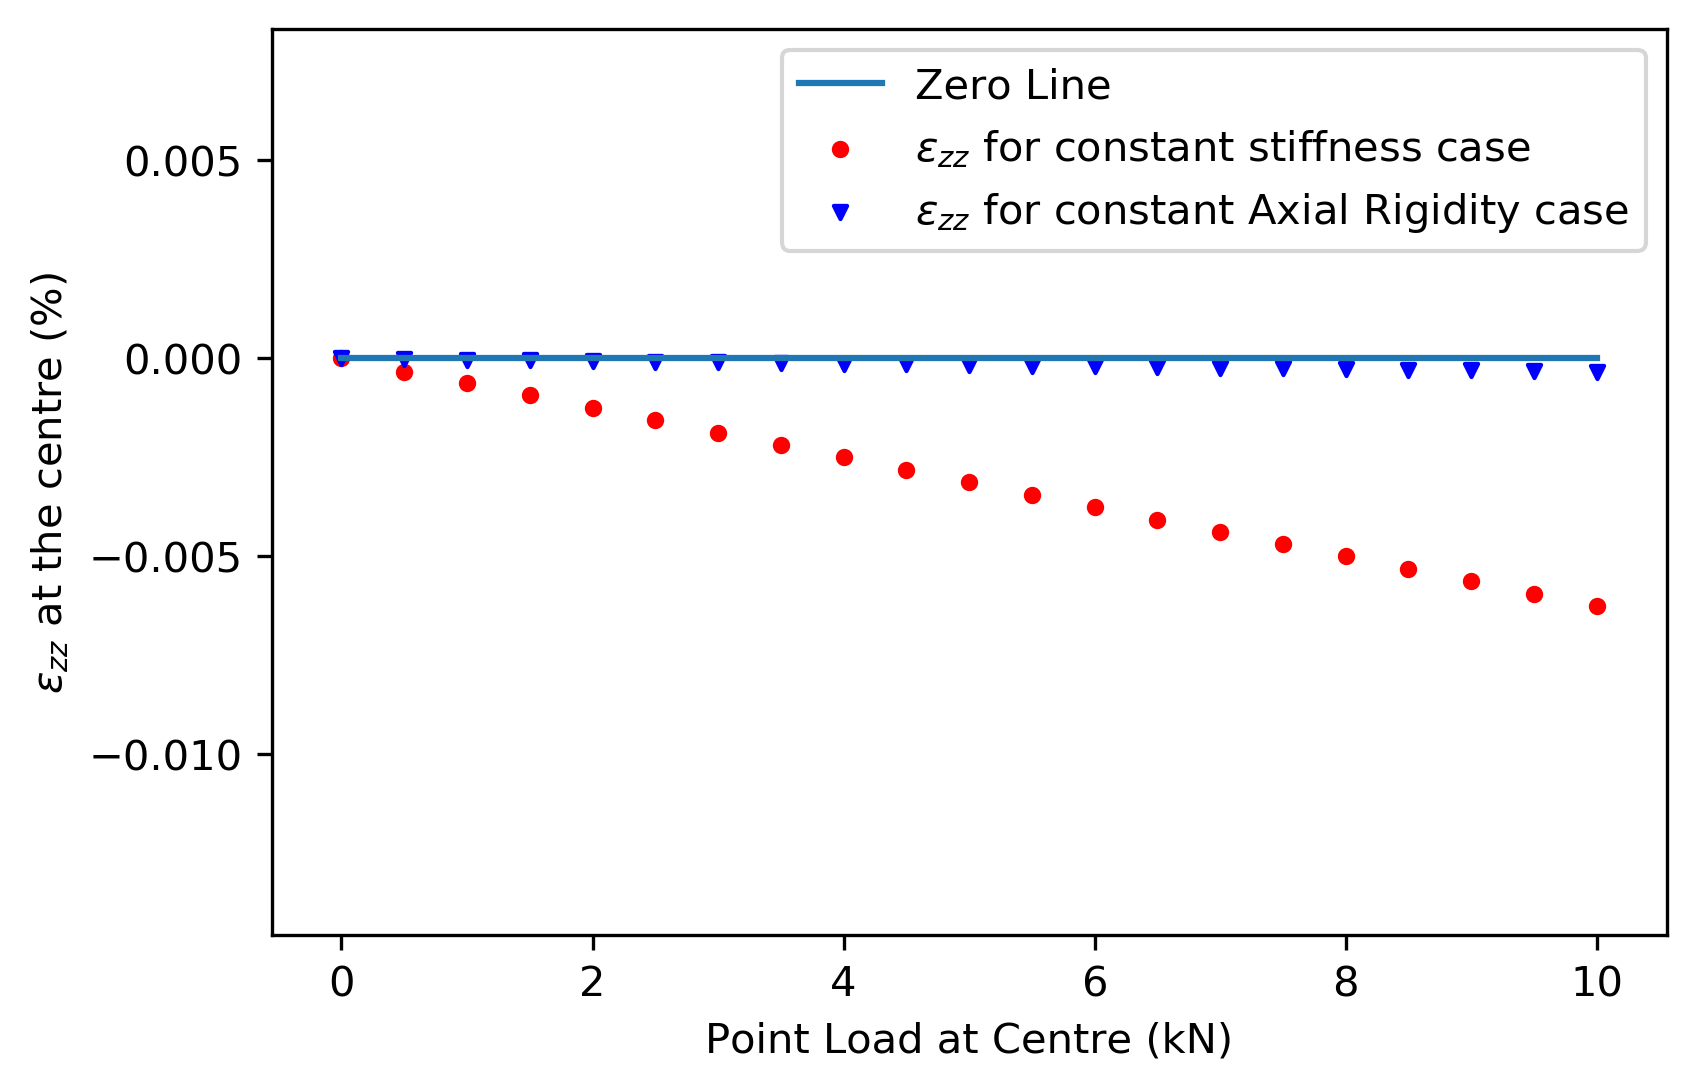
\includegraphics[width = 0.9\textwidth]{Figures/M2_b_strain.png}
    \caption{Model 2 - Type B - $\epsilon_{zz}$ with respect to Point Load at centre}
    \label{fig:M2_b_strain_plt}
\end{figure}


\begin{figure}[!htbp]
    \centering
    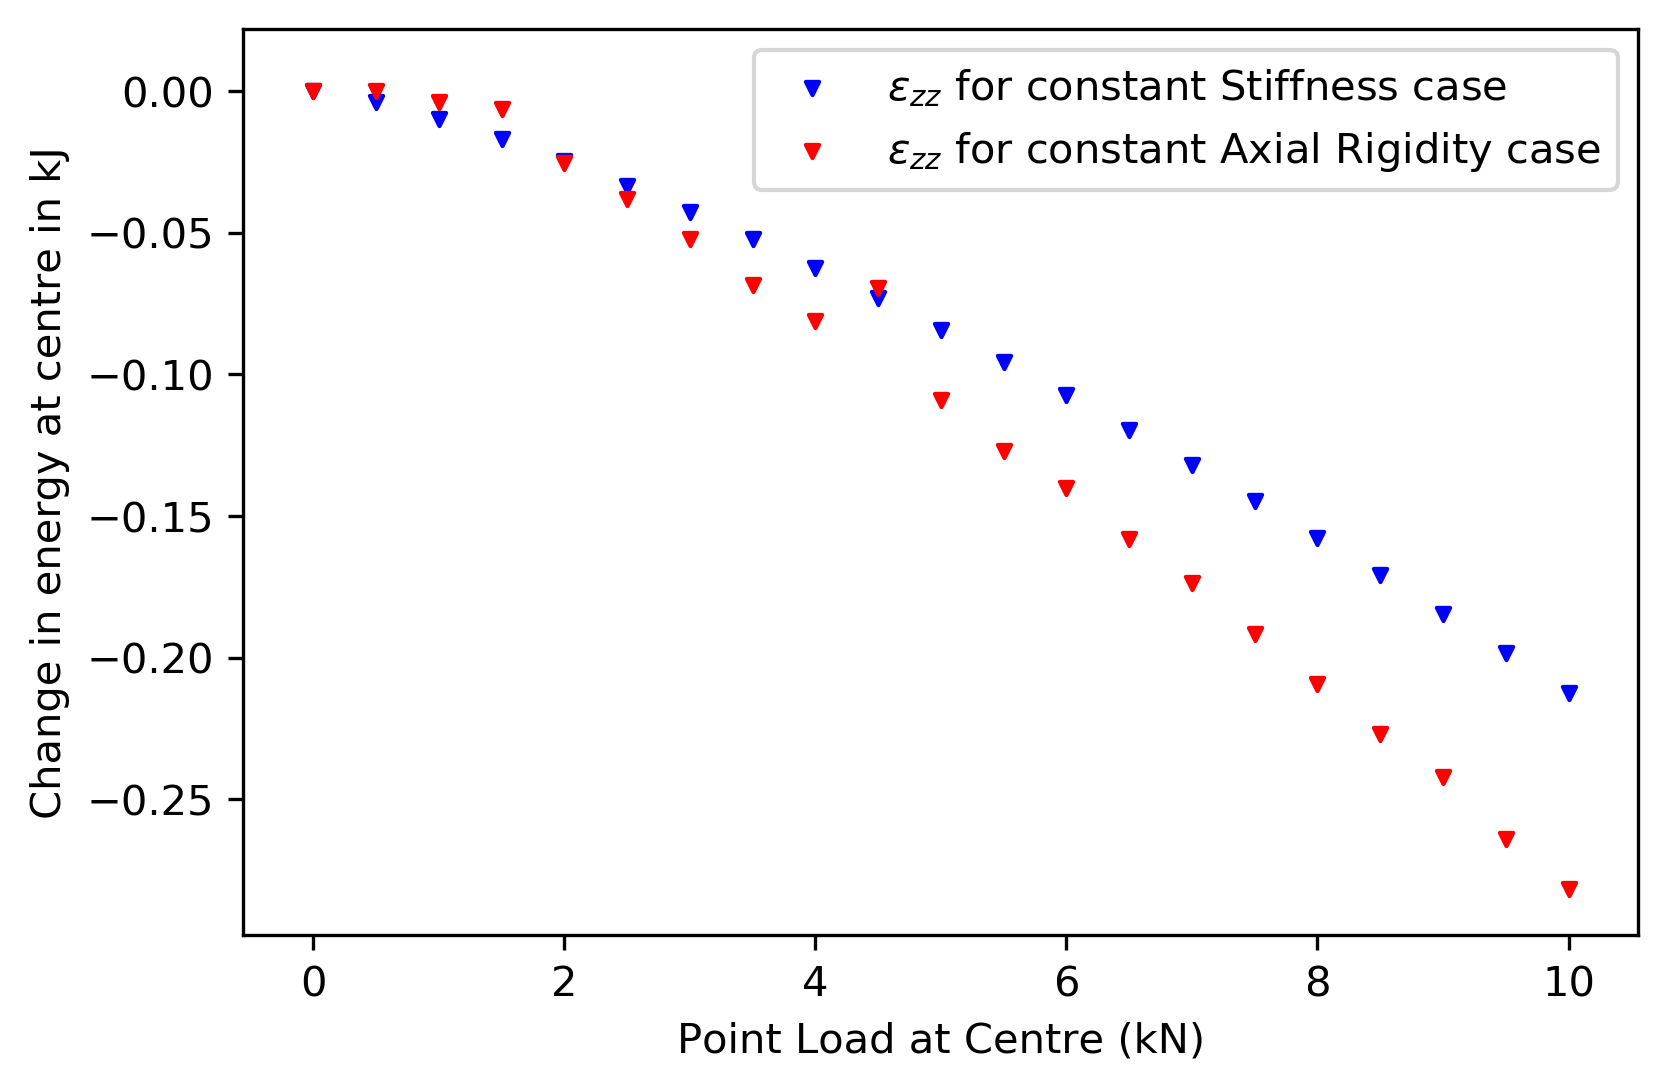
\includegraphics[width = 0.9\textwidth]{Figures/M2_b_energy.png}
    \caption{Model 2 - Type B - Change in Energy with respect to Point Load at centre}
    \label{fig:M2_b_energy}
\end{figure}

 \newpage
 \subsubsection{Model 2 - Type C}
 Model 2 - Type C is 20 x 20 x 2 structure of Model 2 cuboids of dimensions 0.05~m x 0.05~m x 0.01~m. The model is shown in fig~\ref{fig:M2_c_XY} - fig~\ref{fig:M2_c_3D}

\begin{figure}[!htbp]
\begin{minipage}{0.3\textwidth}
    \centering
    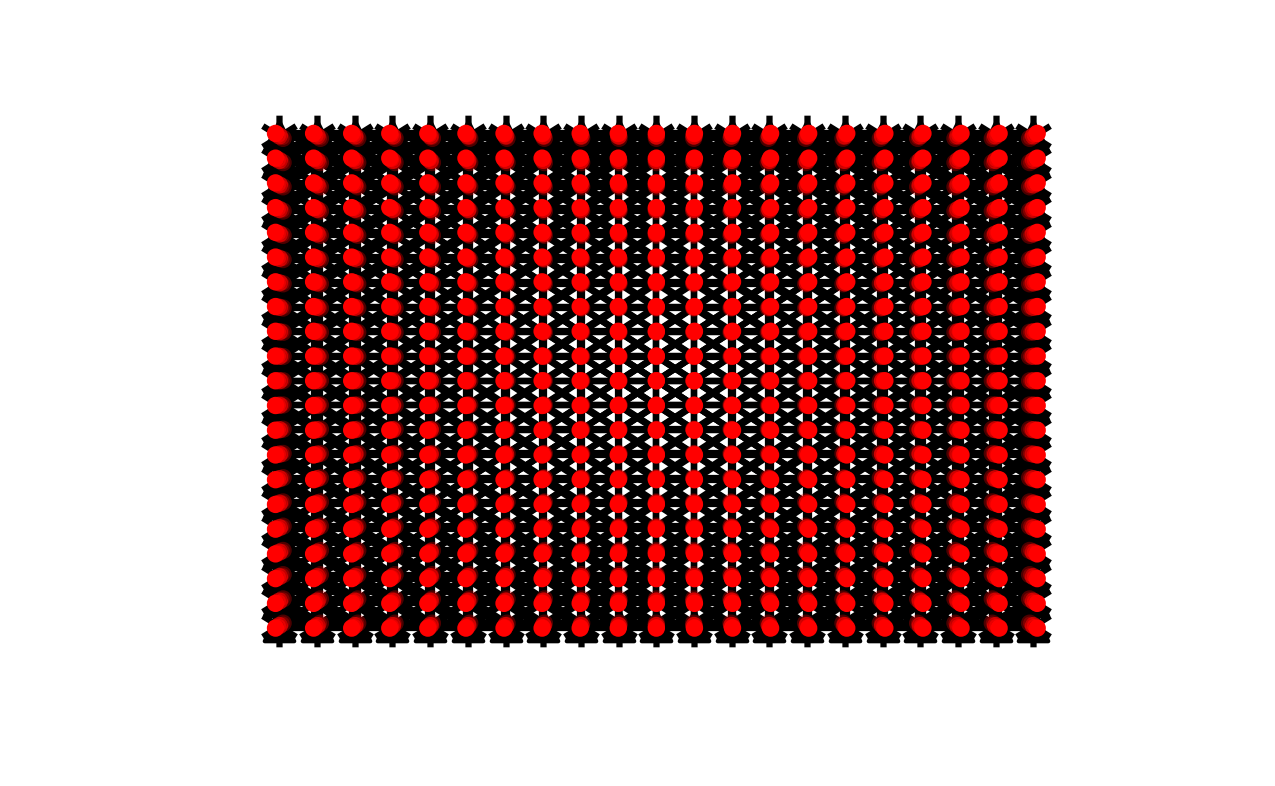
\includegraphics[width = 1\textwidth]{Figures/M2_type_c_XY.png}
    \caption{Model 2 - Type C - XY Projection}
    \label{fig:M2_c_XY}
\end{minipage}
\hspace{5mm}
\begin{minipage}{0.3\textwidth}
    \centering
    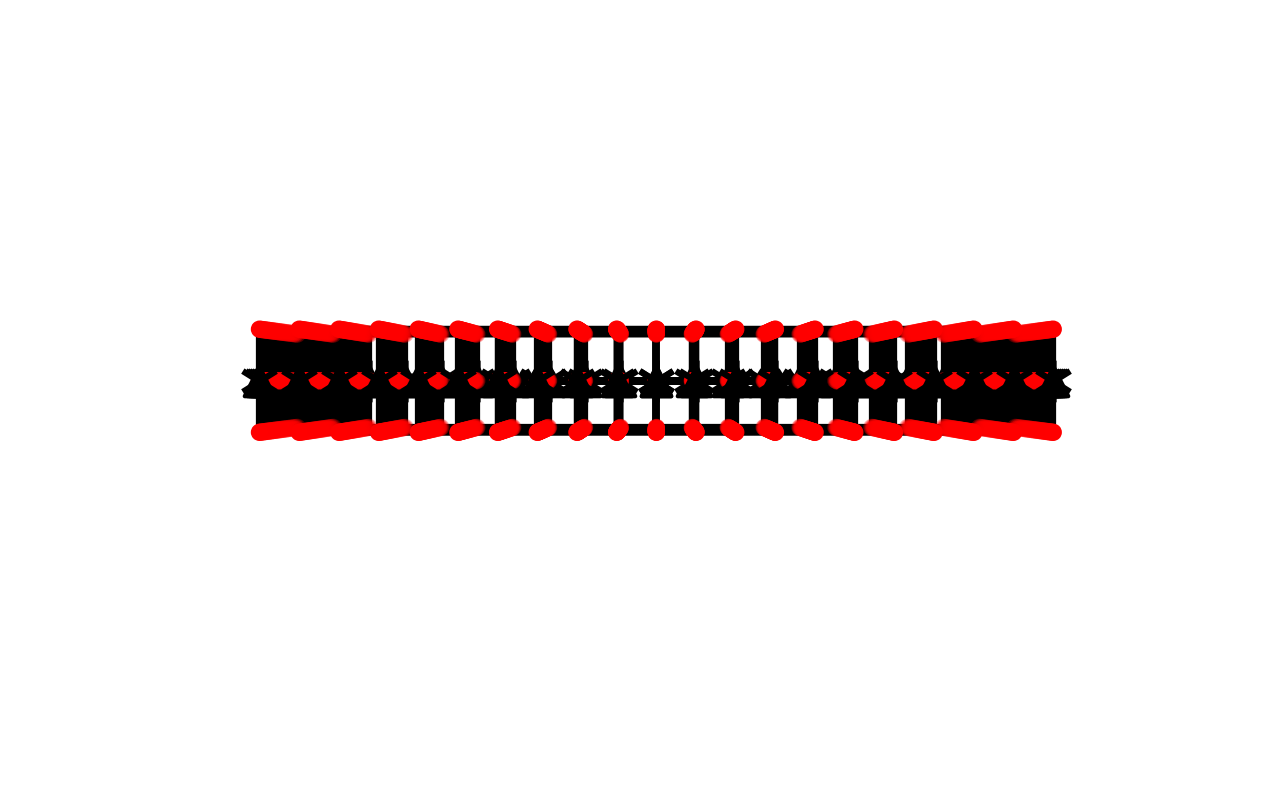
\includegraphics[width = 1\textwidth]{Figures/M2_type_c_YZ.png}
    \caption{Model 2 - Type C - YZ Projection}
    \label{fig:M2_c_YZ}
\end{minipage}
\hspace{5mm}
\begin{minipage}{0.3\textwidth}
    \centering
    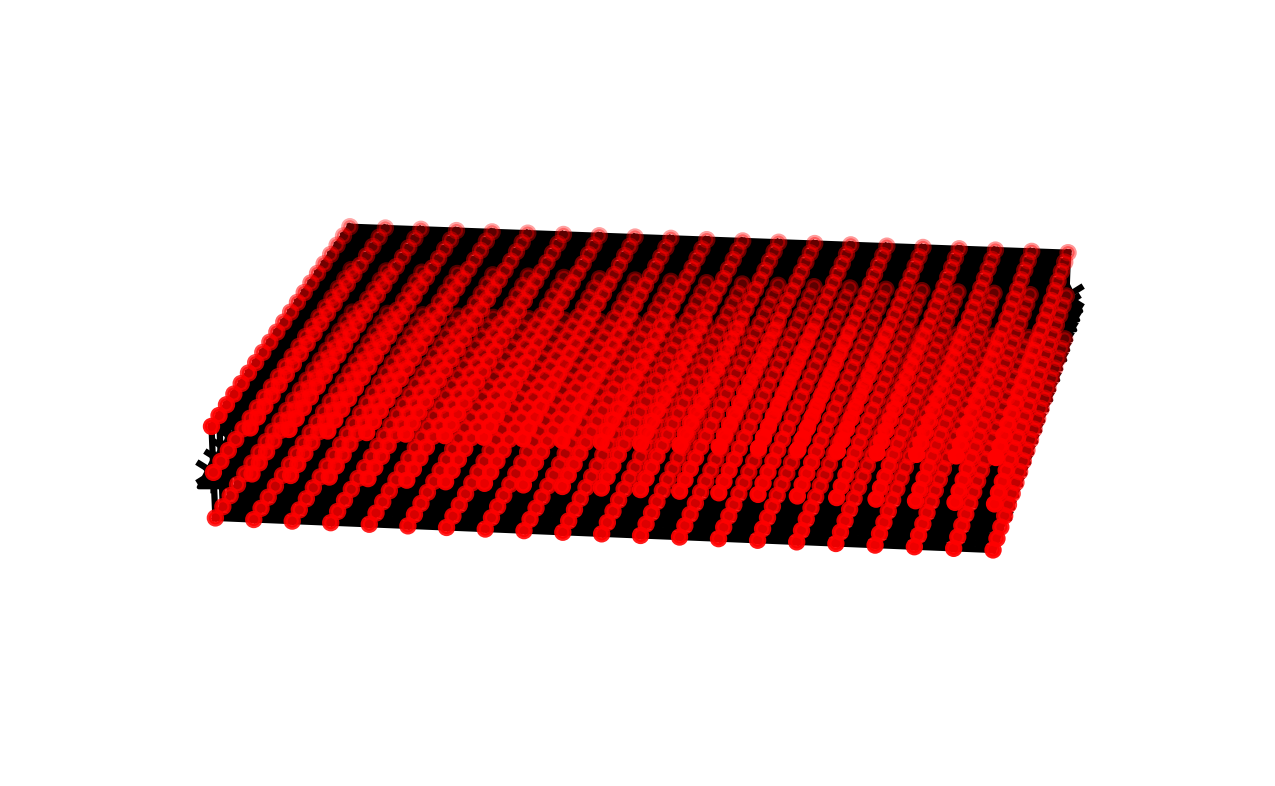
\includegraphics[width = 1\textwidth]{Figures/M2_type_c_3D.png}
    \caption{Model 2 - Type C - 3D View}
    \label{fig:M2_c_3D}
\end{minipage}
\end{figure}

The plots corresponding to Model 2 - Type C are shown in fig~\ref{fig:M2_c_plt} - fig~\ref{fig:M2_c_energy}. For Model 2 Type C case, both, Constant Stiffness and Constant Axial Rigidity study, predict smooth deflection curve and closely resemble each other. However, they both underpredict the deflection compared to those obtained using analytical solutions. 

\begin{figure}[!htbp]
    \centering
    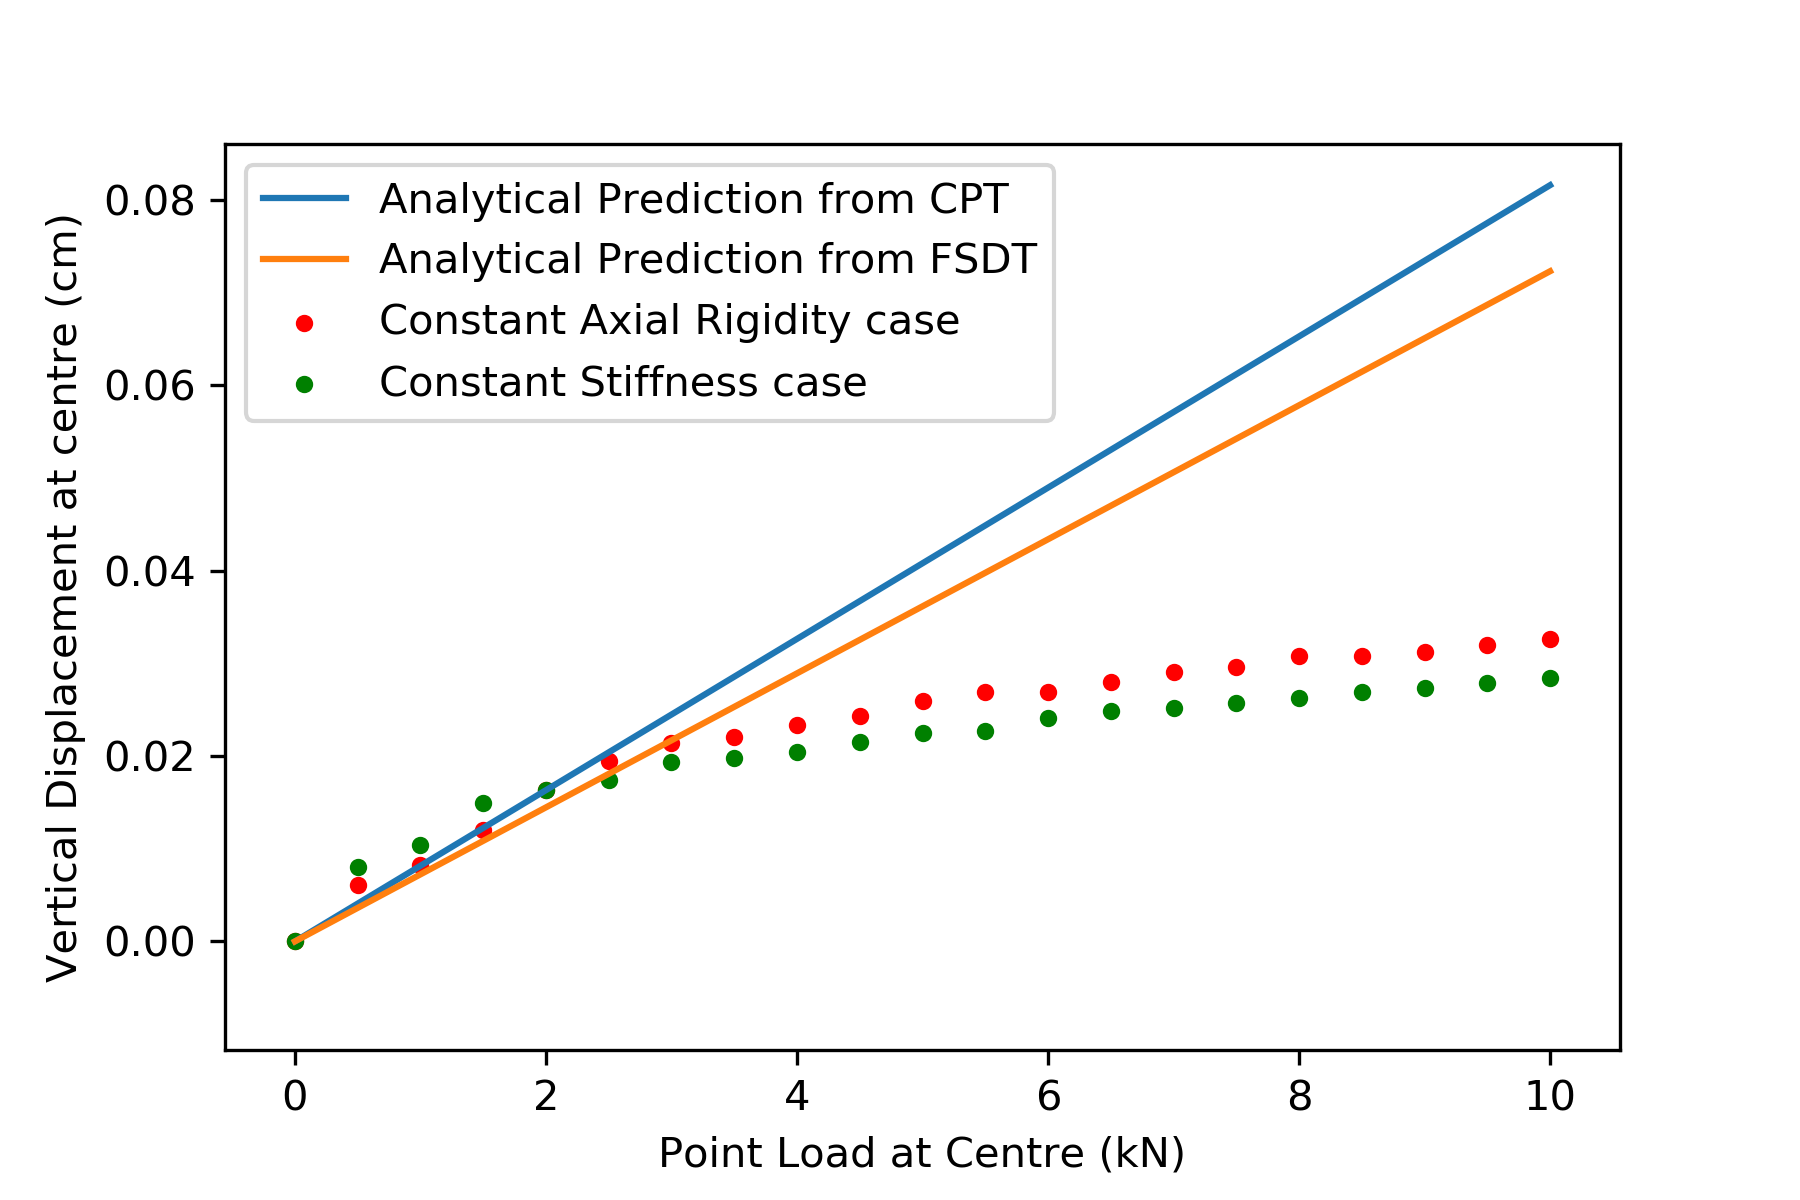
\includegraphics[width = 0.8\textwidth]{Figures/M2_c_plt.png}
    \caption{Model 2 - Type C - vertical Displacement with respect to Point Load at centre}
    \label{fig:M2_c_plt}
\end{figure}

\begin{figure}[!htbp]
    \centering
    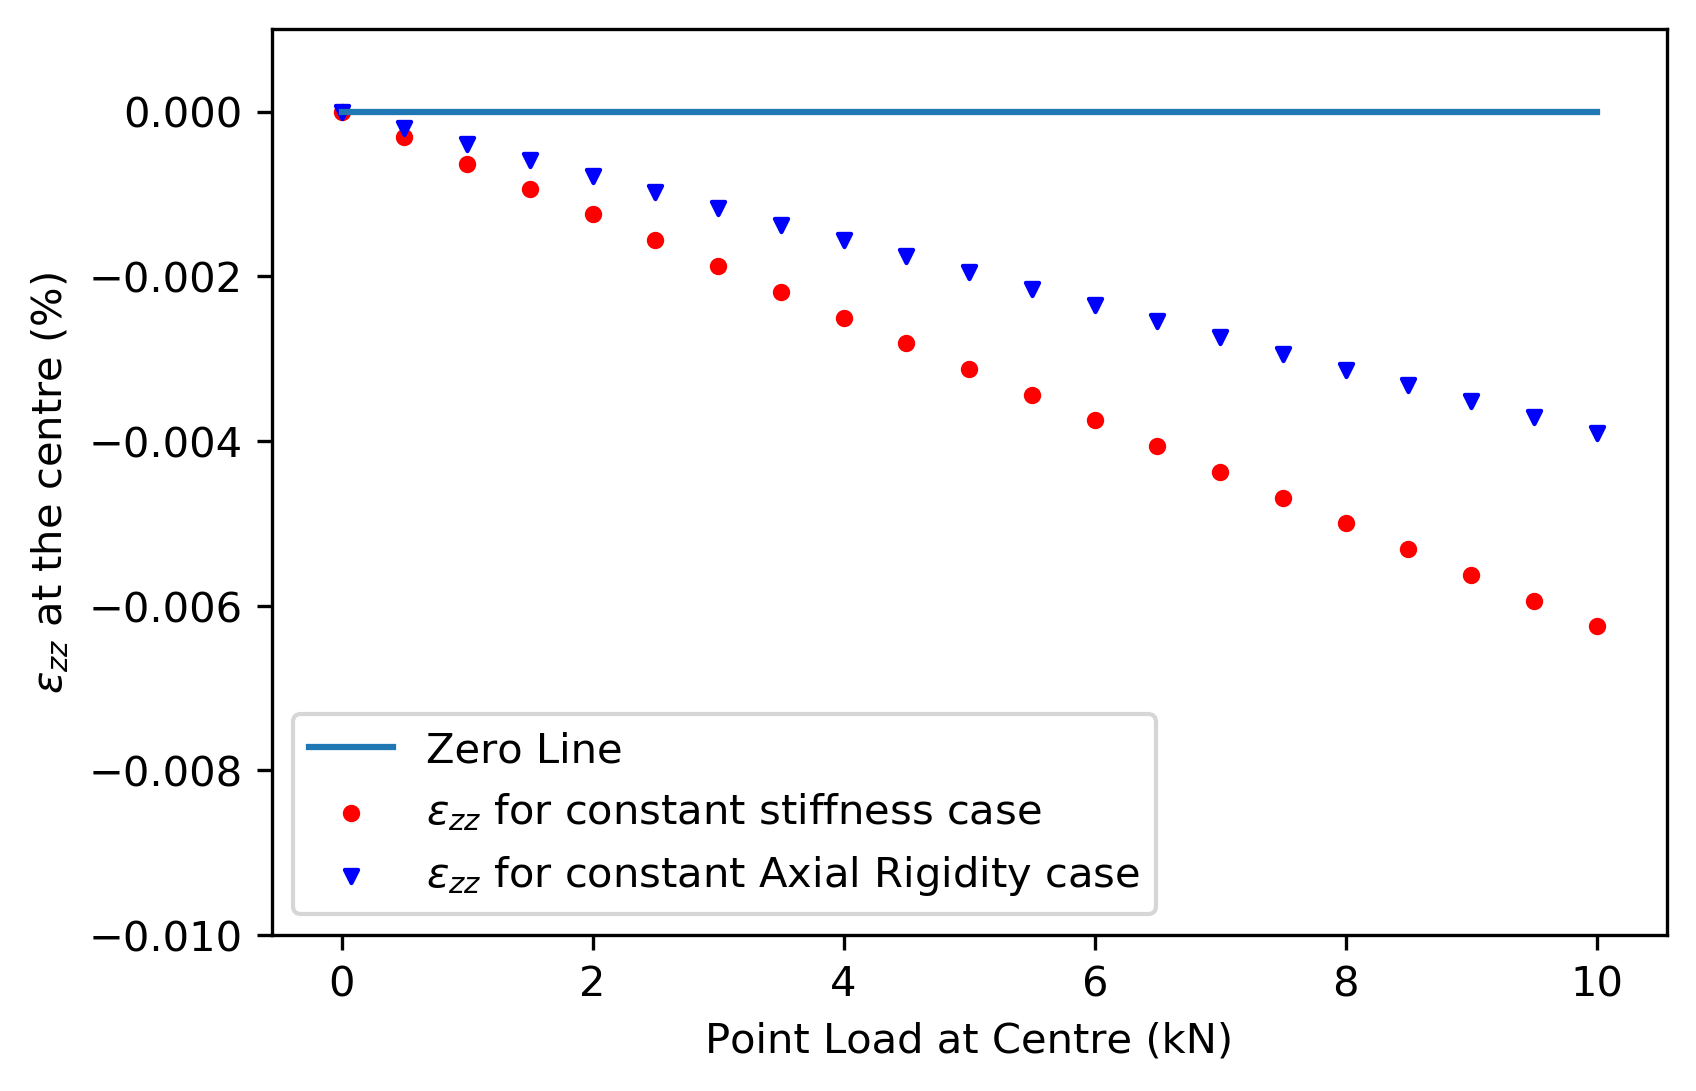
\includegraphics[width = 0.9\textwidth]{Figures/M2_c_strain.png}
    \caption{Model 2 - Type C - $\epsilon_{zz}$ with respect to Point Load at centre}
    \label{fig:M2_c_strain_plt}
\end{figure}

\begin{figure}[!htbp]
    \centering
    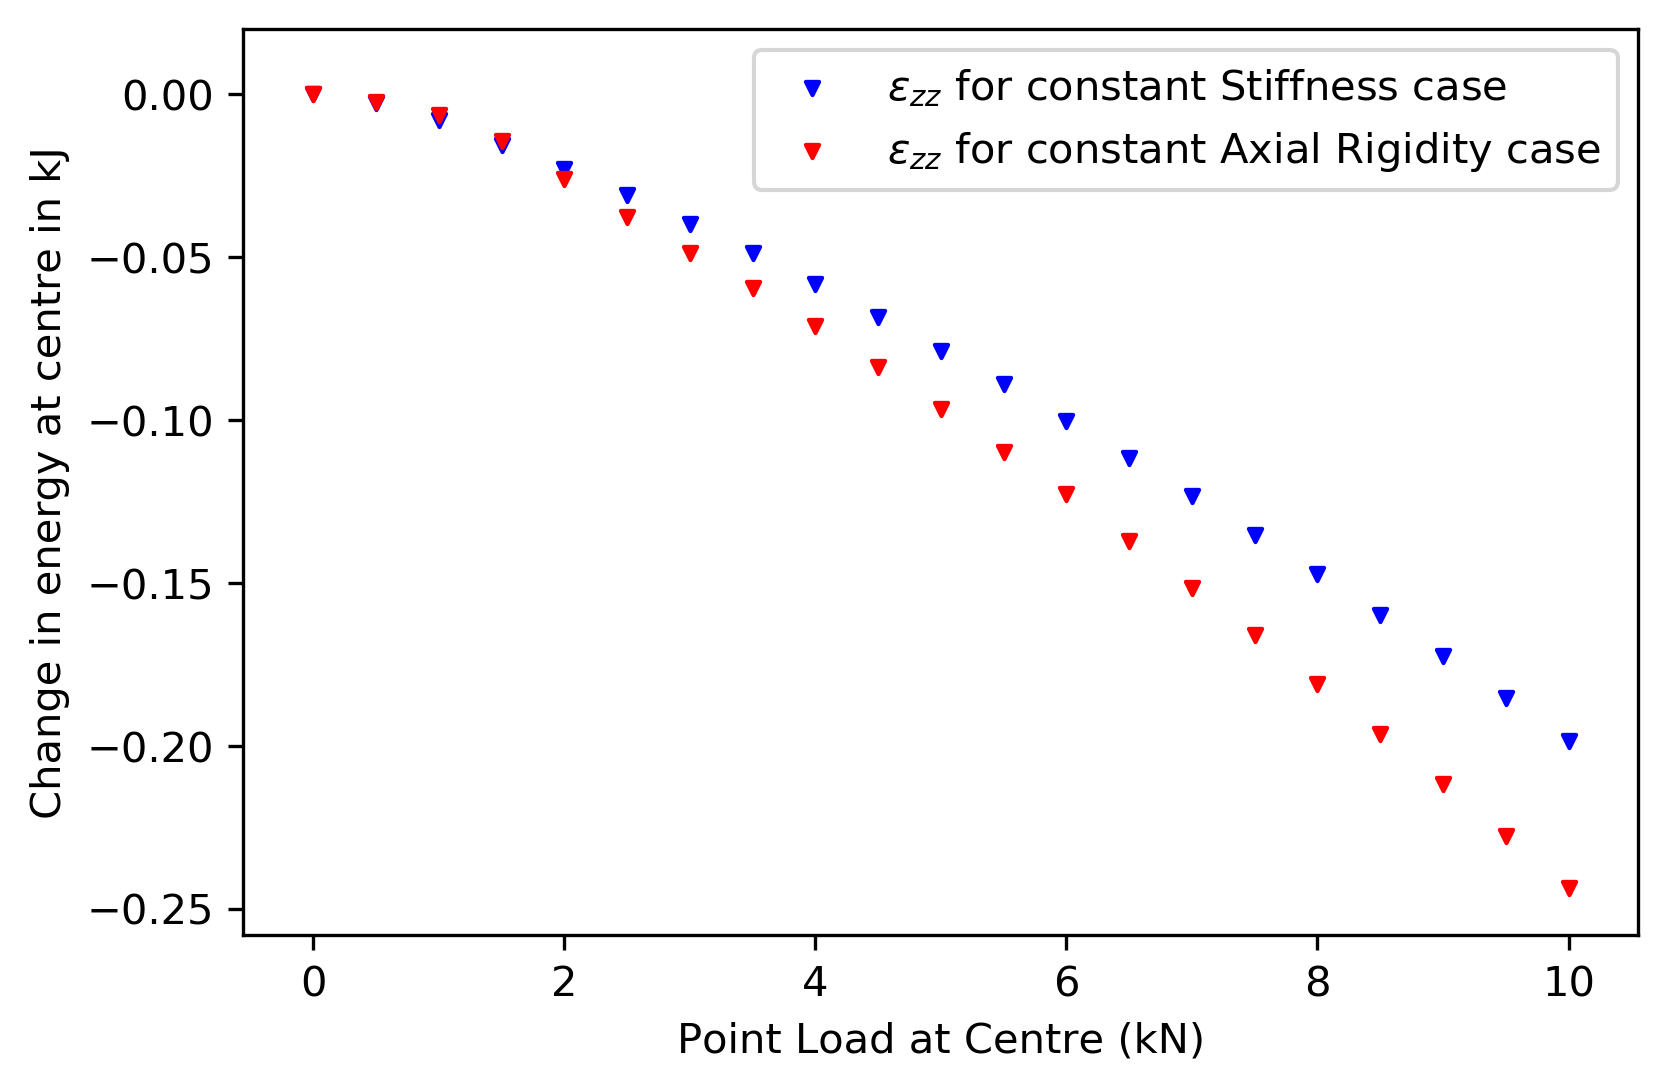
\includegraphics[width = 0.9\textwidth]{Figures/M2_c_energy.png}
    \caption{Model 2 - Type C - Change in Energy with respect to Point Load at centre}
    \label{fig:M2_c_energy}
\end{figure}

Strain for the Model 2 - Type C case are constantly increasing with the applied load as evident from fig~\ref{fig:M2_c_strain_plt}. Strain for the Constant Axial Rigidity case are lower than those of Constant Stiffness case but both of them violate the assumption that $\epsilon_{zz} = 0$ (eq~\ref{eq:CPT_strains_last} and eq~\ref{eq:strain_z_FSDT}). This coupled with non-linear behavior of horizontal spring system under vertical loading result in underestimation of vertical deflections by the model compared to those predicted by analytical theories. The energy profile predicted by the model is also smooth as compared to Model 2 - Type A and Model 2 - Type B indicating that model is numerically stable and matrices involved have low condition number and are well conditioned.

\newpage
\subsection{Model 3}
Model 3 comprises of cuboidal unit cells with in-plane diagonals on top and bottom plane and all body diagonals. Dimension of the plate is 1~m x 1~m x 0.02~m and stiffness of the springs in model are calibrated for displacement at centre for a 2 kN point load applied at centre with displacements at centre of an equivalent plate with $E = 2$ GPa and $\nu = 0.25$).

\subsubsection{Model 3 - Type A}
These models are type 3 model with 4 x 4 x 2 structure of cuboids of dimension 0.25~m x 0.25~m x 0.01~m stacked together as shown in the fig~\ref{fig:M3_a_XY} - fig~\ref{fig:M3_a_3D}.

\begin{figure}[!htbp]
\begin{minipage}{0.3\textwidth}
    \centering
    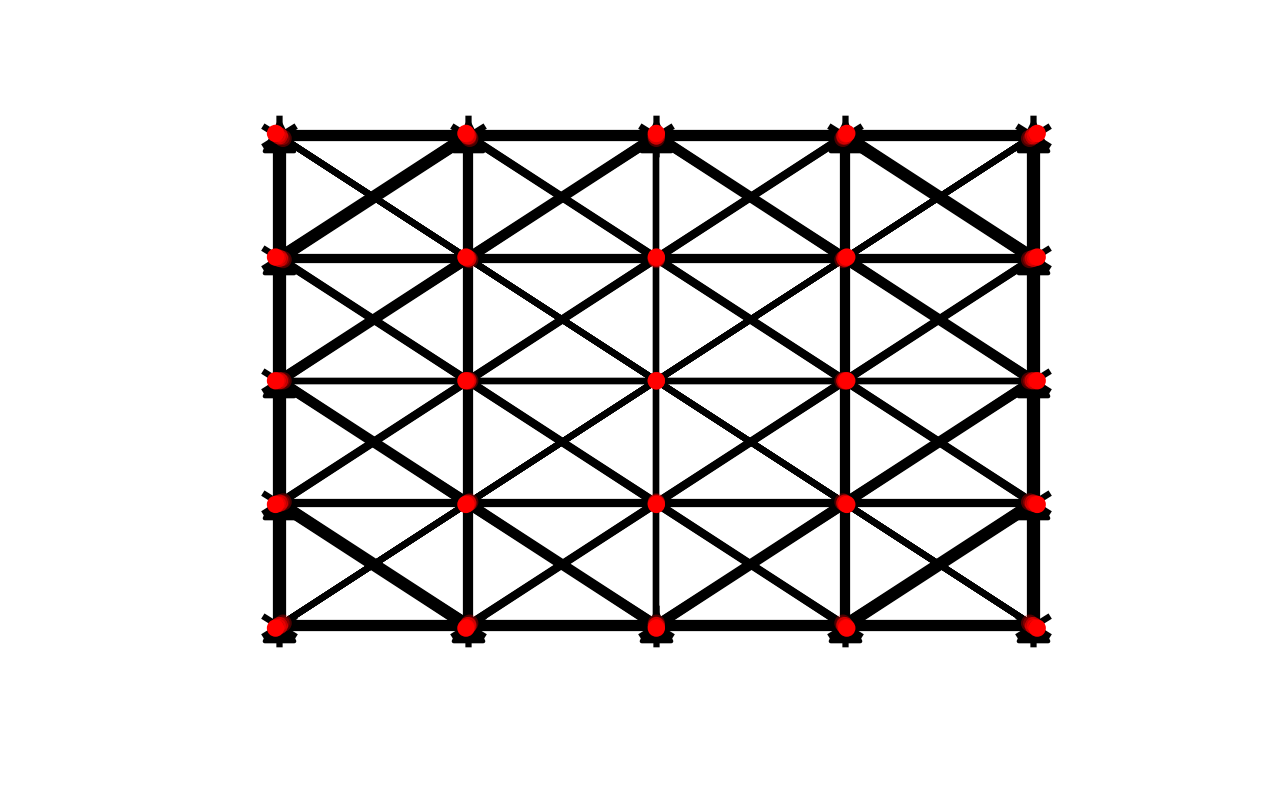
\includegraphics[width = 1\textwidth]{Figures/M3_type_a_XY.png}
    \caption{Model 3 - Type A - XY Projection}
    \label{fig:M3_a_XY}
\end{minipage}
\hspace{5mm}
\begin{minipage}{0.3\textwidth}
    \centering
    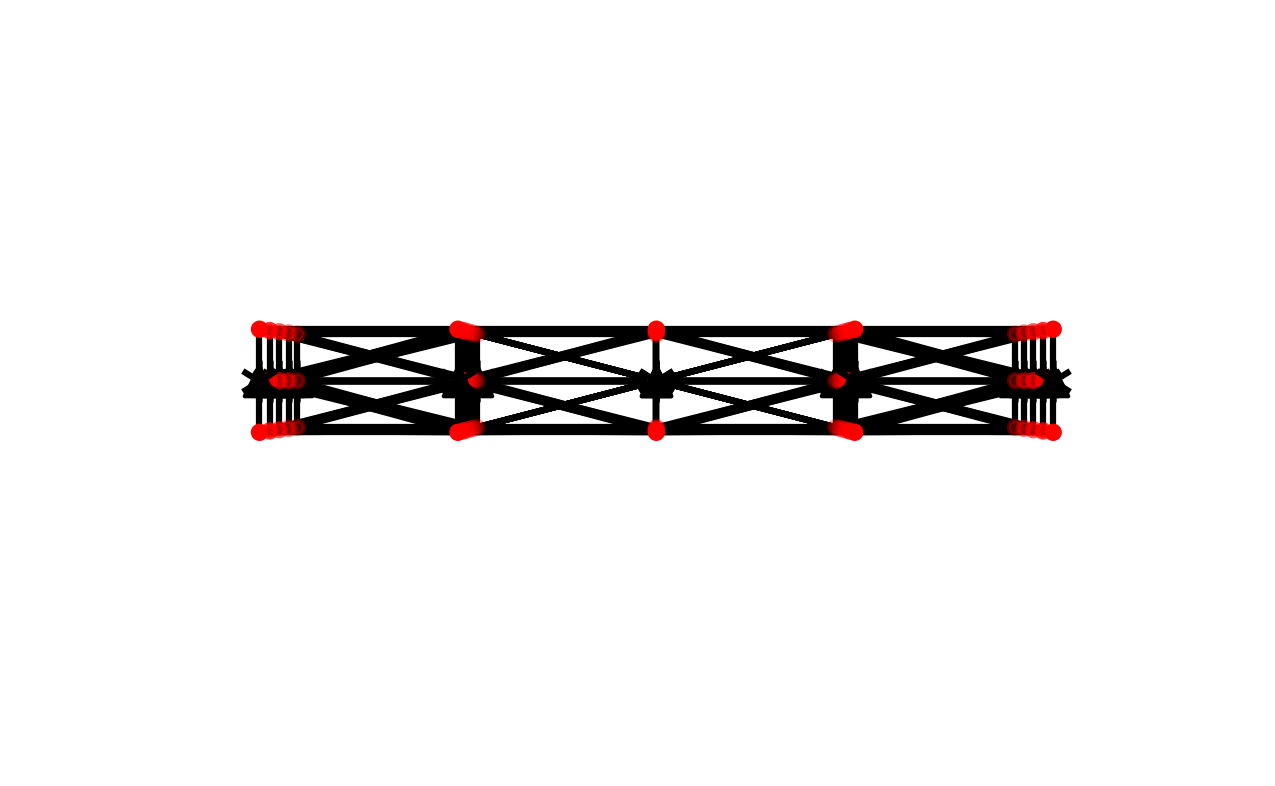
\includegraphics[width = 1\textwidth]{Figures/M3_type_a_YZ.png}
    \caption{Model 3 - Type A - YZ Projection}
    \label{fig:M3_a_YZ}
\end{minipage}
\hspace{5mm}
\begin{minipage}{0.3\textwidth}
    \centering
    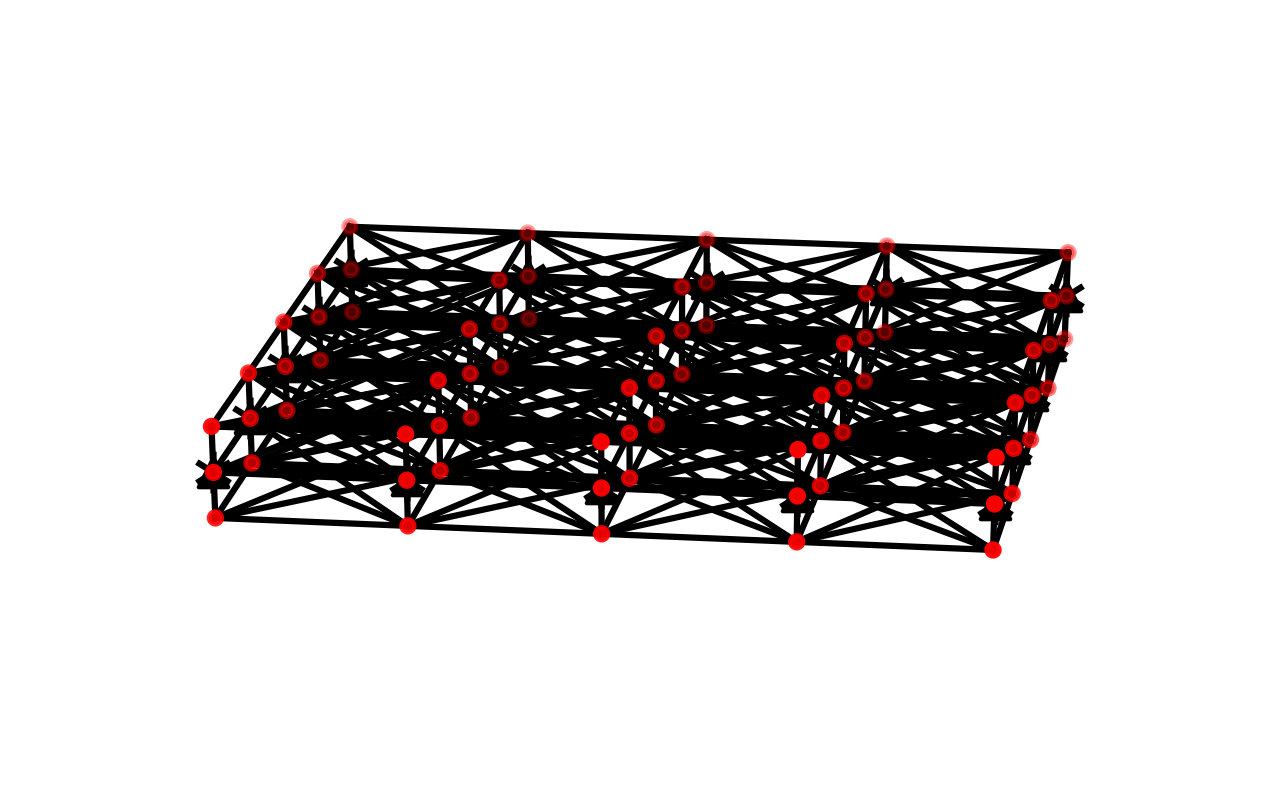
\includegraphics[width = 1\textwidth]{Figures/M3_type_a_3D.png}
    \caption{Model 3 - Type A - 3D View}
    \label{fig:M3_a_3D}
\end{minipage}
\end{figure}

The fig~\ref{fig:M3_a_plt} presents the plots for vertical deflections at centre with respect to point load applied at the centre for Constant Stiffness and Constant Axial rigidity cases. The model predicts very similar deflection for two cases which lies closer to the predictions from the First-order Shear Deformation theory compared to the Classical Plate theory, however these predictions deviate significantly from the analytical predictions. The underestimation of deflection like previous cases can be attribute to non-linear response of horizontal spring system under vertical load. However, one peculiar point to notice is that in fig~\ref{fig:M3_a_strain_plt}, even though the vertical strain for Constant axial rigidity case and Constant stiffness case differ significantly, the vertical deflection at centre predicted by the two at centre are almost equal. Also, for loading of 9 kN under Constant Axial Rigidity case, model is crushed at centre (fig~\ref{fig:M3_a_crushed}) resulting in very high strains. This anomaly might be due to some numerical instability leading to an ill conditioned matrix and hence the irregular strain.

\begin{figure}[!htbp]
    \centering
    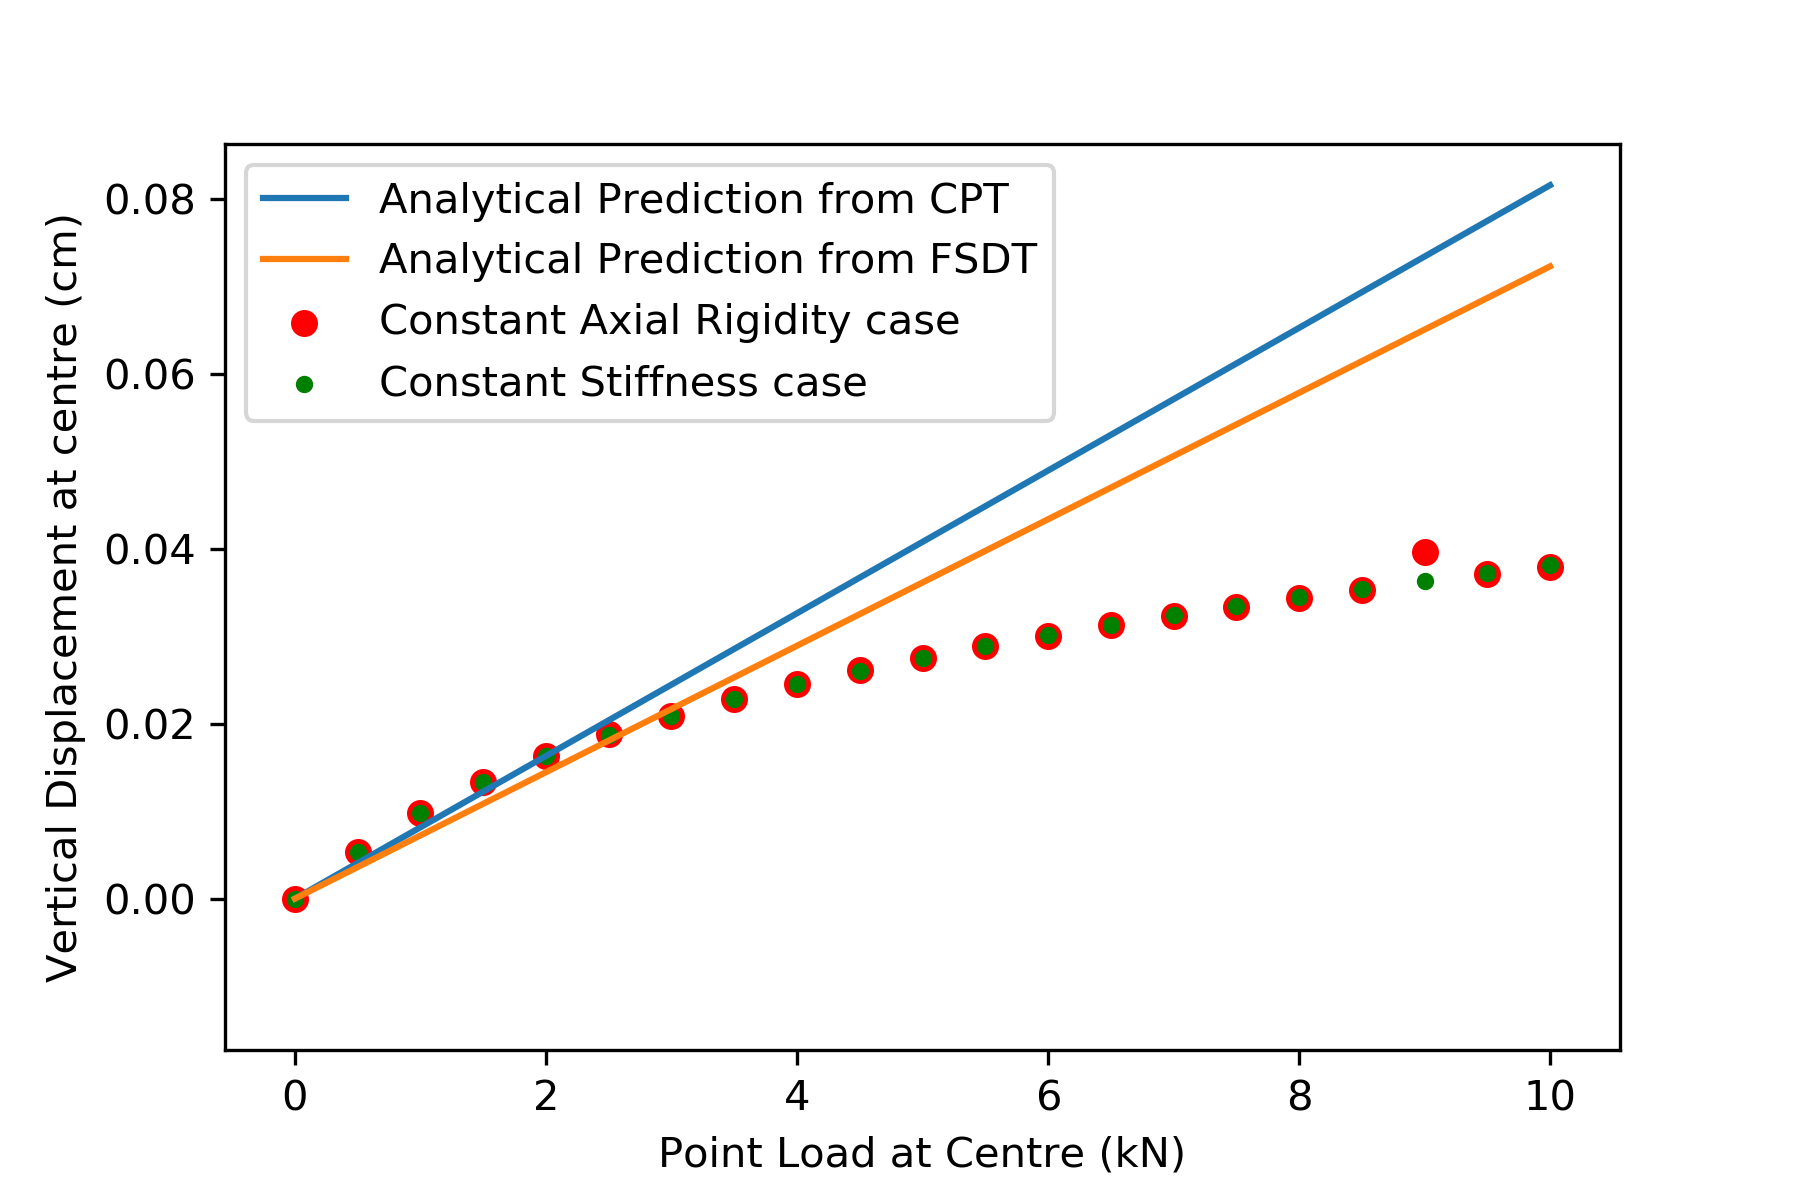
\includegraphics[width = 0.8\textwidth]{Figures/M3_a_plt.png}
    \caption{Model 3 - Type A - vertical Displacement with respect to Point Load at centre}
    \label{fig:M3_a_plt}
\end{figure}

\begin{figure}[!htbp]
    \centering
    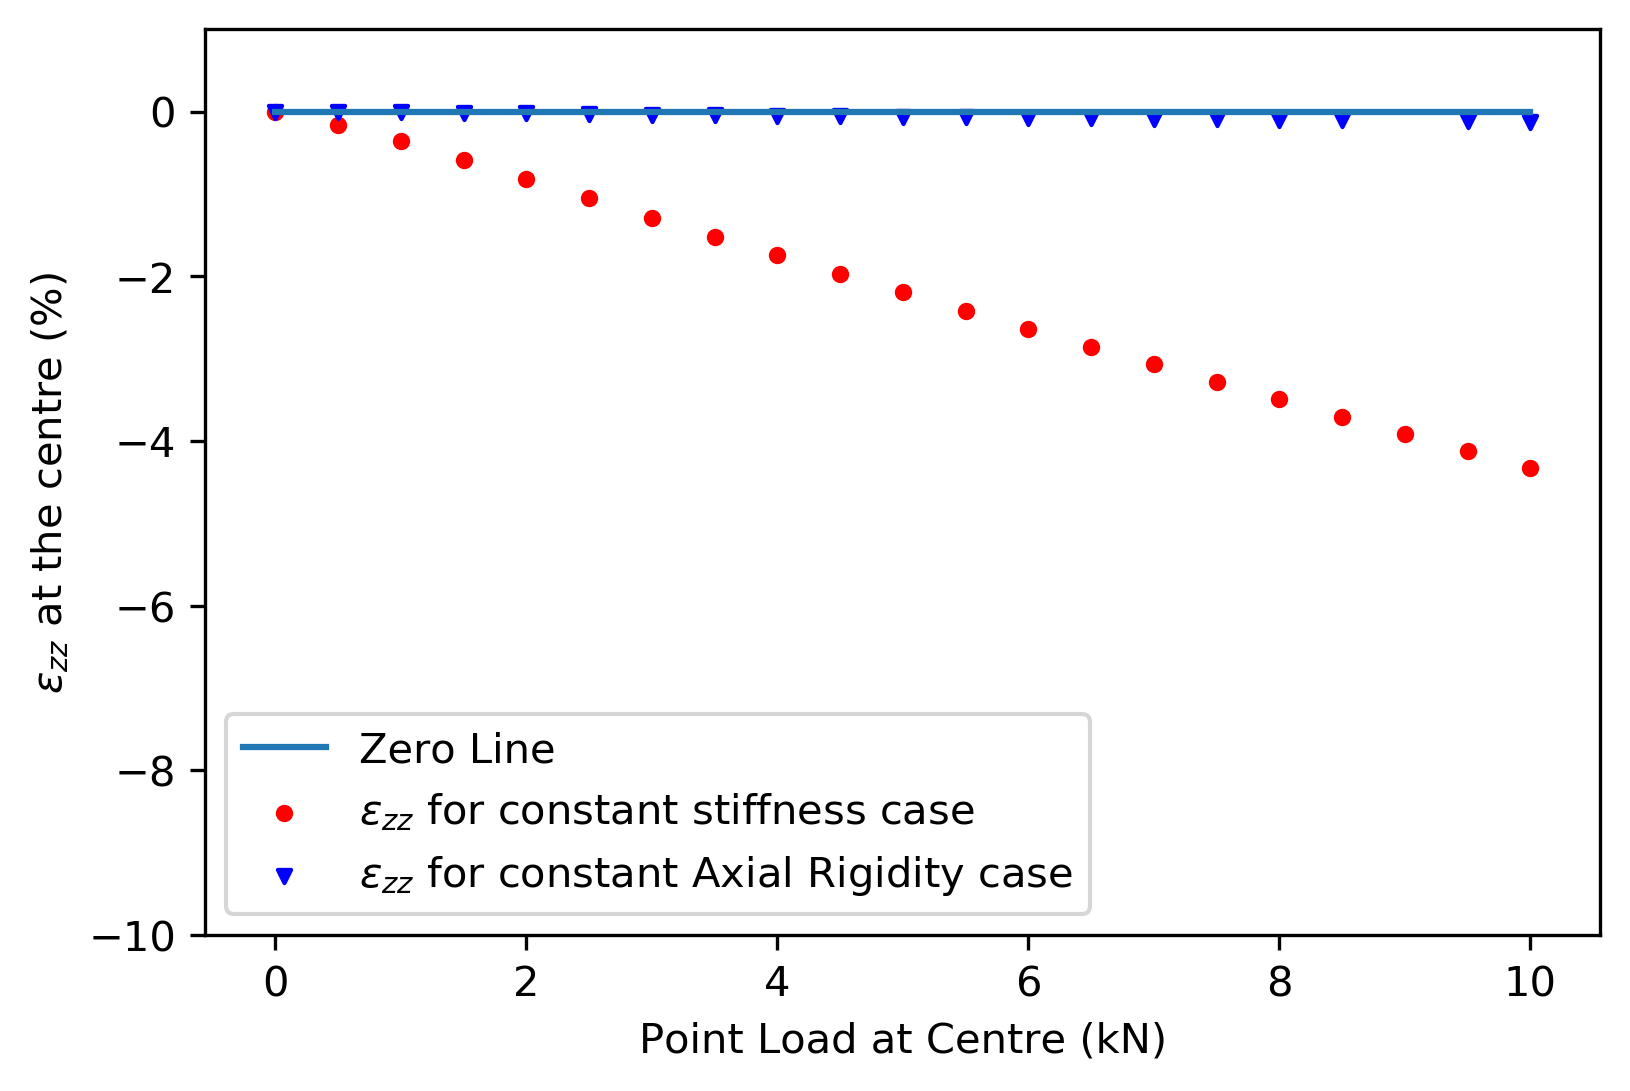
\includegraphics[width = 0.9\textwidth]{Figures/M3_a_strain.png}
    \caption{Model 3 - Type A - $\epsilon_{zz}$ with respect to Point Load at centre}
    \label{fig:M3_a_strain_plt}
\end{figure}

\begin{figure}
    \centering
    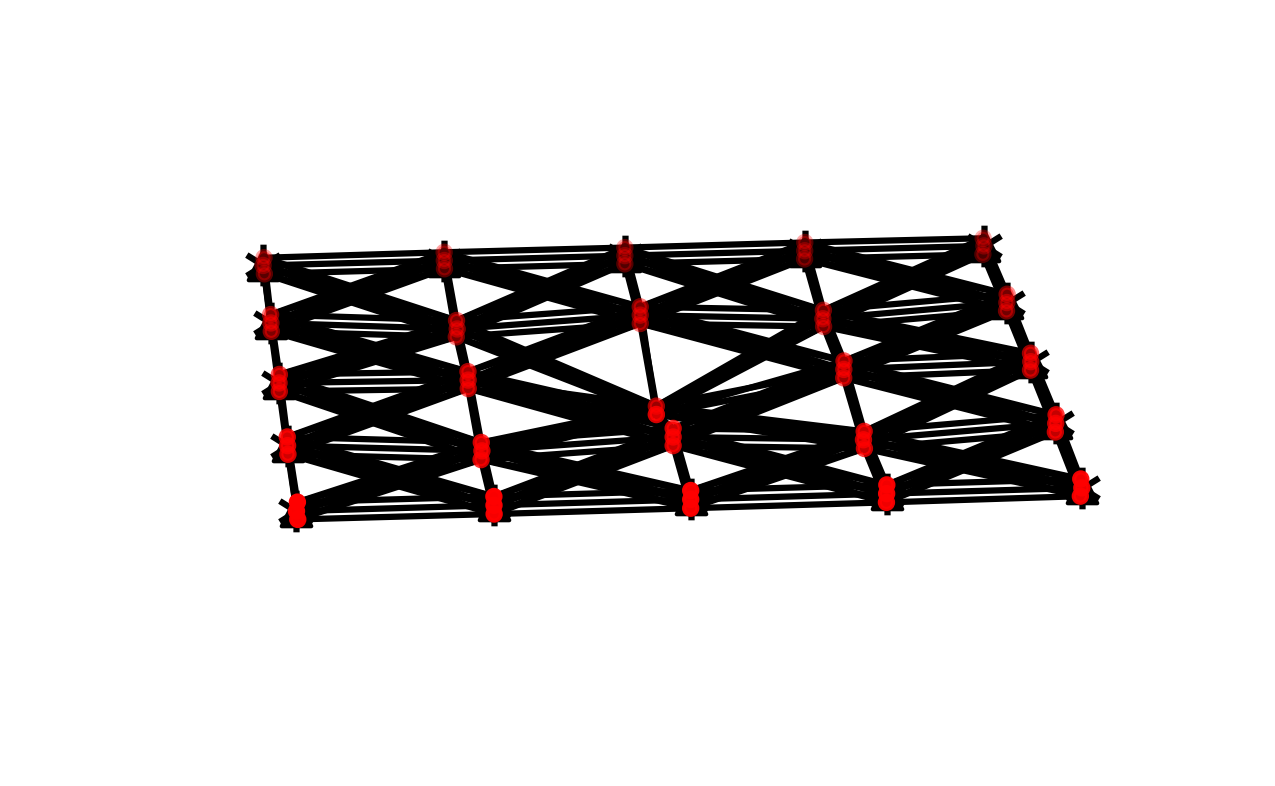
\includegraphics{Figures/M3_a_crushed.png}
    \caption{Model 3 - Type A - Crushed vertical springs under loading of 9 kN resulting in very high $\epsilon_{zz}$}
    \label{fig:M3_a_crushed}
\end{figure}

In fig~\ref{fig:M3_a_energy}, energies in the undeformed state for all forces are zero. Energy profile for Model 3 - Type A is smooth, uniformly decreasing with force, and is almost equal for the case of Constant Axial Rigidity and Constant Stiffness. One anamoly present at the load of 9 kN, as explained earlier, is most probably due to some numerical instability.

\begin{figure}[!htbp]
    \centering
    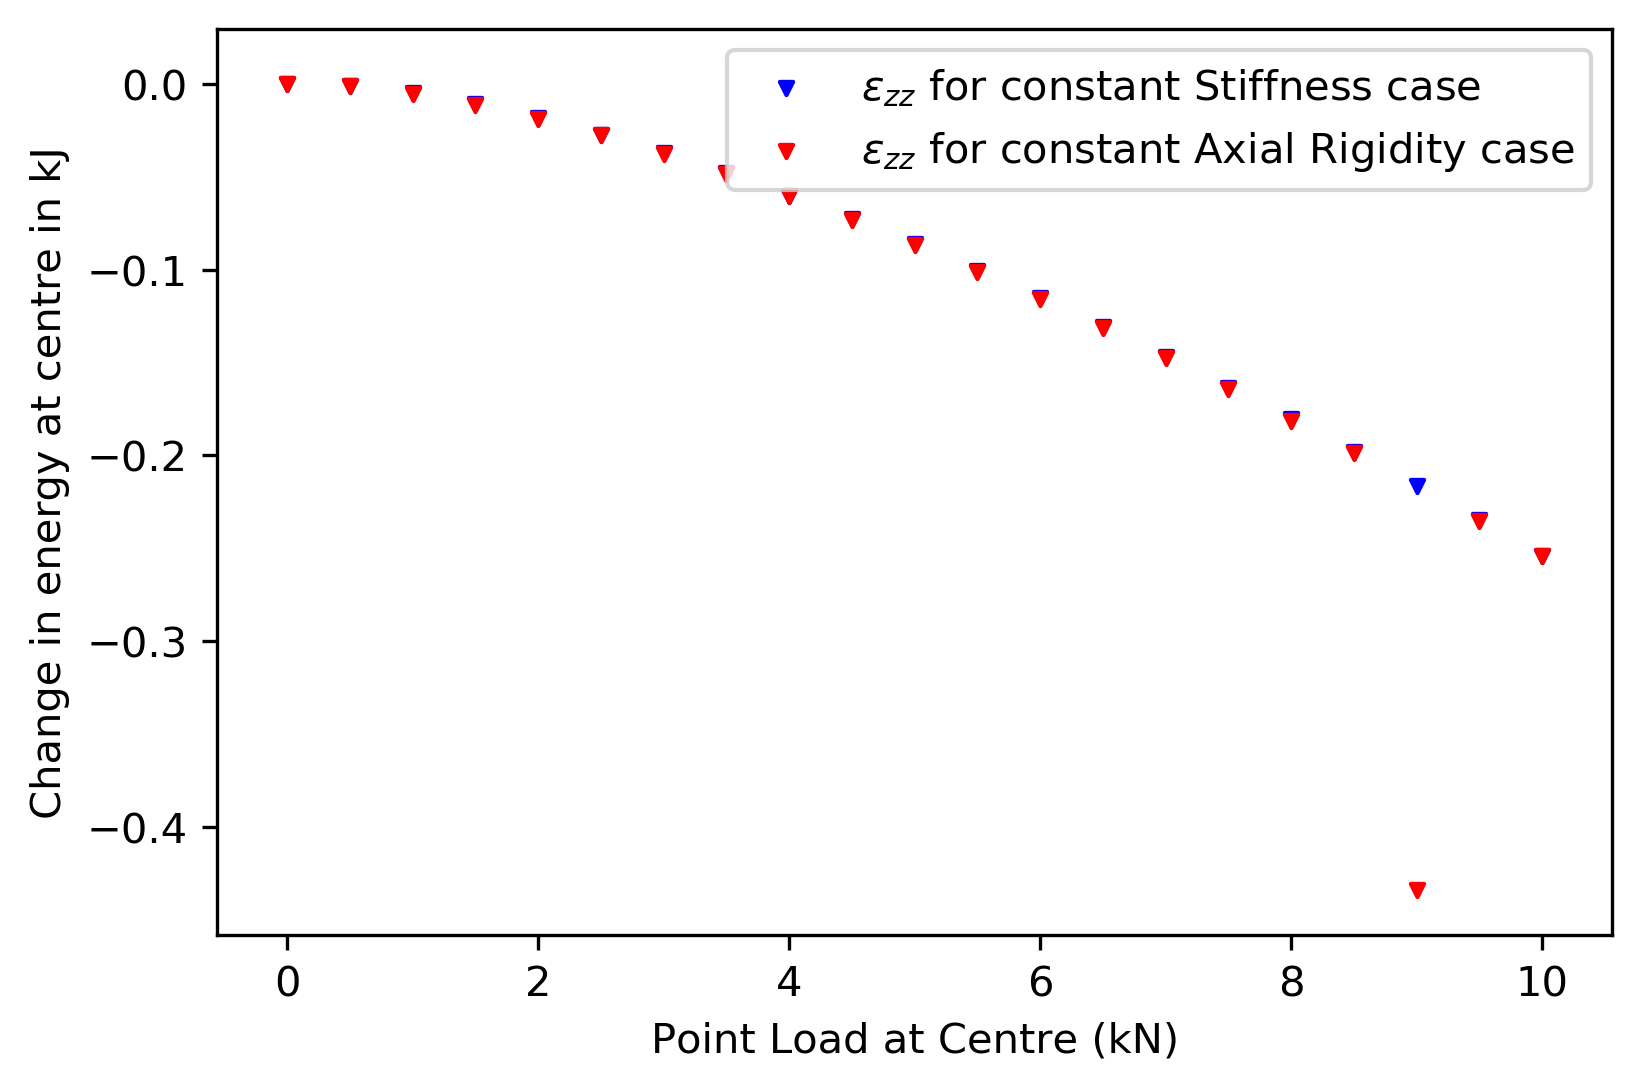
\includegraphics[width = 0.9\textwidth]{Figures/M3_a_energy.png}
    \caption{Model 3 - Type A - Change in Energy with respect to Point Load at centre}
    \label{fig:M3_a_energy}
\end{figure}

\subsubsection{Model 3 - Type B}
Model 3 - Type B is 10 x 10 x 2 structure of Model 2 cuboids of dimensions 0.1~m x 0.1~m x 0.01~m. The model is shown in fig~\ref{fig:M3_b_XY} - fig~\ref{fig:M3_b_3D}

\begin{figure}[!htbp]
\begin{minipage}{0.3\textwidth}
    \centering
    \includegraphics[width = 1\textwidth]{Figures/M3_b_XY.png}
    \caption{Model 3 - Type B - XY Projection}
    \label{fig:M3_b_XY}
\end{minipage}
\hspace{5mm}
\begin{minipage}{0.3\textwidth}
    \centering
    \includegraphics[width = 1\textwidth]{Figures/M3_b_YZ.png}
    \caption{Model 3 - Type B - YZ Projection}
    \label{fig:M3_b_YZ}
\end{minipage}
\hspace{5mm}
\begin{minipage}{0.3\textwidth}
    \centering
    \includegraphics[width = 1\textwidth]{Figures/M3_b_3D.png}
    \caption{Model 3 - Type B - 3D View}
    \label{fig:M3_b_3D}
\end{minipage}
\end{figure}

The plots corresponding to Model 3 - Type B are shown in fig~\ref{fig:M3_b_plt} - fig~\ref{fig:M3_b_energy}. The deflection predictions for Constant Stiffness case and Constant Axial Rigidity case are almost equal and assume a parabolic shape similar to that in Model 3 - Type A. However, the strains for this case are considerably higher than those of Model 3 - Type A despite the vertical deflection at centre being almost same. Also, the vertical strain corresponding to the Constant Axial Rigidity cases are much lower than those of Constant Stiffness case.

\begin{figure}[!htbp]
    \centering
    \includegraphics[width = 0.8\textwidth]{Figures/M3_b_plt.png}
    \caption{Model 3 - Type B - vertical Displacement with respect to Point Load at centre}
    \label{fig:M3_b_plt}
\end{figure}

\begin{figure}[!htbp]
    \centering
    \includegraphics[width = 0.9\textwidth]{Figures/M3_b_strain.png}
    \caption{Model 3 - Type B - $\epsilon_{zz}$ with respect to Point Load at centre}
    \label{fig:M3_b_strain_plt}
\end{figure}

The energy profile as shown in the fig~\ref{fig:M3_b_energy} is almost same as that of Model 3 - Type A (fig~\ref{fig:M3_a_energy}), except for the anomaly in Model 3- Type A profile at 9 kN load. 

\begin{figure}[!htbp]
    \centering
    \includegraphics[width = 0.9\textwidth]{Figures/M3_b_energy.png}
    \caption{Model 3 - Type B - Change in Energy with respect to Point Load at centre}
    \label{fig:M3_b_energy}
\end{figure}

 \newpage
 \subsubsection{Model 3 - Type C}
 Model 3 - Type C is 20 x 20 x 2 structure of Model 3 cuboids of dimensions 0.05~m x 0.05~m x 0.01~m. The model is shown in fig~\ref{fig:M3_c_XY} - fig~\ref{fig:M3_c_3D}

\begin{figure}[!htbp]
\begin{minipage}{0.3\textwidth}
    \centering
    \includegraphics[width = 1\textwidth]{Figures/M3_type_c_XY.png}
    \caption{Model 3 - Type C - XY Projection}
    \label{fig:M3_c_XY}
\end{minipage}
\hspace{5mm}
\begin{minipage}{0.3\textwidth}
    \centering
    \includegraphics[width = 1\textwidth]{Figures/M3_type_c_YZ.png}
    \caption{Model 3 - Type C - YZ Projection}
    \label{fig:M3_c_YZ}
\end{minipage}
\hspace{5mm}
\begin{minipage}{0.3\textwidth}
    \centering
    \includegraphics[width = 1\textwidth]{Figures/M3_type_c_3D.png}
    \caption{Model 3 - Type C - 3D View}
    \label{fig:M3_c_3D}
\end{minipage}
\end{figure}

The plots corresponding to Model 3 - Type C are shown in fig~\ref{fig:M3_c_plt} - fig~\ref{fig:M3_c_energy}. This model predicts deflection accurately in accordance with the First-order Shear Deformation theory and lies very close to Classical plate theory. In this model, both, Constant Axial Rigidity case and Constant Stiffness case predict the deflections accurately as can be seen from fig~\ref{fig:M3_c_plt}. The Constant Axial Rigidity case has much lower strain than constant Stiffness case, however in both the case, vertical strains are much smaller than those of Model 3 - Type A and Model 3 - Type B.

\begin{figure}[!htbp]
    \centering
    \includegraphics[width = 0.8\textwidth]{Figures/M3_c_plt.png}
    \caption{Model 3 - Type C - vertical Displacement with respect to Point Load at centre}
    \label{fig:M3_c_plt}
\end{figure}

\begin{figure}[!htbp]
    \centering
    \includegraphics[width = 0.9\textwidth]{Figures/M3_c_strain.png}
    \caption{Model 3 - Type C - $\epsilon_{zz}$ with respect to Point Load at centre}
    \label{fig:M3_c_strain_plt}
\end{figure}

As evident from the scale of Y-Axis of fig~\ref{fig:M3_c_energy}, the decrease in energy in Model C - Type 3 study is much smaller than other models and cases. Here as well, the Constant Axial Rigidity case and Constant Stiffness case, follow each other very closely.

\begin{figure}[!htbp]
    \centering
    \includegraphics[width = 0.9\textwidth]{Figures/M3_c_energy.png}
    \caption{Model 3 - Type C - Change in Energy with respect to Point Load at centre}
    \label{fig:M3_c_energy}
\end{figure}

\newpage
\section{Conclusion}

Based on the studies above, following conclusions can be drawn:
\begin{enumerate}
    \item It is observed that vertical deflections predicted by Constant Axial Stiffness case are generally higher and closer to analytical solutions as compared to those predicted by Constant Stiffness case. Also, the vertical normal strains in model under the Constant Axial Rigidity strain are closer to zero as compared to the Constant Stiffness case. This justifies the importance of the assumption that $\epsilon_{zz} = 0$ in the results of analytical solution and how squeezing of plate under the concentrated vertical loading leads to lowering of vertical deflection at the centre of the plate.
    \item The magnitude of energy change is generally higher for the Constant Axial Rigidity case compared to Constant Axial Rigidity case. This result can be attributed to the higher displacements that the vertically applied force undergoes under Constant Axial Rigidity case. For higher deflection, springs are stretched more and this tends to increase the energy system but it is overcompensated by the work of vertical springs leading to equilibrium at higher displacement as opposed to the Constant Stiffness case.
    \item It can be observed that increasing the number of nodes and springs (or equivalently breaking the plate into more number of cells), i.e. moving from Type A system to Type C systems, the displacement profiles become more regular and the predictions from the Constant Stiffness case and Constant Axial Rigidity case come closer to each other. Also adding in-plane diagonals and body diagonals, i.e. moving from Model 1 to Model 3, has a effect of regularizing and taking predictions closer to the analytical solutions, especially when going from Model 2 to Model 3. This increase in accuracy of the model might be due to bending stiffness that is added to model by using body diagonals. Model 1 and Model 2 do not have any direct connection between two layers and vertical springs provide second order reaction forces for small displacement between planes.
    \item The strains in vertical direction ($\epsilon_{zz}$) are generally higher for Constant Stiffness case than Constant Axial rigidity case. As the number of node and springs are increased, i.e. as we move from Type A to Type C models, vertical strain increases (except in case of Model 3 where vertical strain decreases on moving from Type B to Type C). Moreover, strains increase on moving from Model 1 to Model 3 as the diagonal springs are added. Also, Moving from Type A models to Type C models, the cases in which vertical strains are very high increase. All this indicates that at times it is energetically, at least locally, more favourable to crush the vertical springs in the centre rather than distributing the energy between springs of the horizontal layers.
    \item It is observed that out of Type A, Type B, and Type C Models, Type B has the highest discrepancy between strains predicted by Constant Stiffness and Constant Axial rigidity case. Also Type B models, although marginally, have less regularity compared to Type A and Type C. This indicated some kind of numerical instability in between at Type B Models as we move from Type A models to Type C Models.
    \item The energy profile for Models of all type are mostly uniform and have a predictable pattern. The difference between energy predictions for a given loading by Constant Axial Rigidity case and Constant Stiffness Case appears to increase as one moves from Type A models to Type C models. In most of the cases, the increased discrepancy is due to changes in energies change predicted by Constant Axial Rigidity case while the energy change prediction for Constant Stiffness case remains almost same among models for a given load.
    \item Interestingly, time taken by the program to minimize the energy for model is less than the time taken for minimizing the energy of model 2 despite the increased number of springs. This suggests presence of some kind of numerical stability in type 3 models compare to type 2 models.
    \item While most of the models agree with analytical solution at low loads, they deviate significantly from the analytical solution at higher loads. Model 3 - Type C which provides the deflection results matching very well at all loads has few peculiar properties which are highlighted below.
    \begin{enumerate}
        \item Magnitude of energy change in model 3 - Type C under any given load is much smaller than energy changes in all the other Type and Model despite the fact that the displacements predicted by Model 3 - Type C predicts higher deflections at the centre. This means that although the vertical load does more work, it is compensated by the energy developed in the springs and hence the system has much lower energy change compared to other types and models.
        \item Even though the strains are higher than some of the other cases and differ significantly for Constant Strain and Constant Axial Rigidity case, the energies predicted under any given vertical loading are small compared to other type and models and very close to each other for two cases.
    \end{enumerate}
\end{enumerate}

\section{Limitations of Model and Suggested Improvements}
\label{sec:Limitations}
Following this study, few short comings of the models and possible ways to remedy the situation are pointed out in the following points.
\begin{enumerate}
    \item We can the violation of the assumption $\epsilon_{zz} = 0$ for almost all the models. In some cases the vertical springs are crushed resulting in strains higher than 50\% and are source of errors and deviation from the analytical results. There are two ways in which this problem can be tackled:
    \begin{enumerate}
        \item Providing the vertical springs with stiffness orders of magnitude higher than the horizontal springs. This provides more flexibility to vary vary vertical spring stiffness to simulate different kinds of situations. However, large differences in orders of magnitude of horizontal and vertical springs result in ill conditioned problems which are prone to numerical inaccuracy and instability (as can be seen in some of the figures above). Also this leads to higher computation time and effort.
        \item An alternate way of modelling the $\epsilon_{zz} = 0$ behavior is use this as constraint in the optimization problem. Constraint can be formulated as show in eq~\ref{eq:constraint_for_epsilon}. This prevents the changes in the length of vertical springs and enforce the $\epsilon_{zz} = 0$ assumption. However, this constraint is non linear, and while the optimization algorithm used in the study (L-BFGS-B) can handle the bound constraint, it can not handle non linear constraints. The problem formulated with the constraint shown in eq~\ref{eq:constraint_for_epsilon} will need another constrained non linear optimization algorithm such as Sequential Quadratic Programming (SQP) and will also need take higher computing time and effort.
        \begin{equation}
            \sum_{i \in Z} (l_i - l_{0i})^2 = 0
            \label{eq:constraint_for_epsilon}
        \end{equation}
        Where $Z$ is set of all the vertical springs and $l_i$ and $l_{0i}$ are the actual and natural length of the $i^{th}$ spring.
    \end{enumerate}
    \item In the design function for minimization problem, some kind of regularization function can be added. This will enforce the deformed plate in assuming a smooth shape instead of rectangular tessellation which will resemble more closely with the actual plates.
    \item Model 2 can be modified to include in-plane diagonals in the vertical layers since it will help in maintaining $\epsilon_{zz} = 0$ assumption.
\end{enumerate}
